
\documentclass[a4paper,11pt,]{book}
\usepackage[paperwidth=17cm, paperheight=22.5cm, bottom=2.5cm, right=2.5cm]{geometry}
\usepackage{amssymb,amsmath,amsthm} %paquete para símbolo matemáticos
\usepackage[spanish]{babel}
%\usepackage[latin1]{inputenc}
\usepackage[utf8]{inputenc} %Paquete para escribir acentos y otros símbolos directamente
%\usepackage[T1]{fontenc}
%\usepackage{textcomp}
\usepackage{enumerate}
\usepackage{graphicx}
\usepackage{subfigure} % subfiguras
\usepackage{float}
\usepackage{array}
\usepackage[Lenny]{fncychap}
\usepackage{longtable,multirow,booktabs}
\usepackage[nouppercase]{scrpage2} % encabezados
\usepackage{cite}% para contraer referencias
\usepackage{cancel}
\usepackage{float}
\usepackage[noblocks]{authblk}
\usepackage{multirow}
\providecommand{\abs}[1]{\lvert#1\rvert}
\providecommand{\norm}[1]{\lVert#1\rVert}


\pagestyle{scrheadings} %encabezados
\setlength{\headheight}{1.1\baselineskip} %encabezados

%\usepackage{subfig} %para poner subfiguras
\graphicspath{{graficas/}} %En qué carpeta están las imágenes
\usepackage[nottoc]{tocbibind}
\usepackage[pdftex,
            pdfauthor={CRISTIAN ALFREDO OSPINA DE LA CRUZ},
            pdftitle={TÍTULO DE LA TESIS},
            pdfsubject={ÁREA DE LA TESIS},
            pdfkeywords={PALABRAS CLAVE},
            pdfproducer={Latex con hyperref},
            pdfcreator={pdflatex}]{hyperref}

\usepackage{emptypage}
\newcommand{\grad}{$^{\circ}$}
\begin{document}

% Atencion: la division en silabas se hace atendiendo al criterio de que
% en una linea queden al menos tres letras de la palabra que se divide.
% He dejado algunas excepciones a esta regla (ex-pe-ri-men-tal, por ejemplo)

% Recordar que aqui solo se pueden poner palabras que no lleven acentos
% ni dieresis. Tampoco palabras extranjeras que lleven otros simbolos
% de este tipo.

% Aqui he acopiado las palabras que en algun documento, ya sea de Fisica o no,
% el TeX las ha dividido mal.

\hyphenation{aban-do-na-mos
             abso-lu-ta-men-te
             ace-le-ra-do
             ace-le-ra-cio-nes
             ace-le-ra-dor
             ace-le-ra-do-res
             ace-le-ra-da
             ace-le-ra-das
             aco-pla-do
             aco-pla-dos
             aco-pla-mien-to
             aco-pla-mien-tos
             ac-tua-li-za-da
             ac-tua-li-za-do
             ac-tua-li-zar
             ae-ro-puer-to
             a-gra-de-ci-mien-to
             a-gra-de-ci-mien-tos
             Ana-li-ce-mos
             ana-li-za-da
             ana-li-za-das
             ana-li-za-do
             ana-li-za-dos
             ana-li-za-ron
             an-te-rior
             an-te-rio-res
             aproxi-ma-da
             aproxi-ma-da-men-te
             aproxi-ma-do
             aproxi-me
             aquel
             aque-lla
             aque-llas
             aque-llos
             arri-bar
             asi-me-trica
             asi-mis-mo
             aso-cia-da
             aso-cia-das
             aso-cia-do
             aso-cia-dos
             aspec-to
             aspec-tos
             aten-dien-do
             auto-fre-cuen-cia
             auto-fre-cuen-cias
             auto-si-mi-lar
             auto-si-mi-la-ri-dad
             auto-va-lor
             auto-va-lo-res
             auto-vec-tor
             auto-vec-to-res
             auxi-liar-nos}

\hyphenation{ba-lan-ce
             ba-lan-ces
             ban-da
             ban-das
             barre-ras
             bidi-men-sio-nal
             bidi-men-sio-na-les
             carac-te-ri-za
             carac-te-ri-zar
             ca-rre-ra
             ca-rre-ras
             car-te-sia-na
             car-te-sia-no
             cas-te-lla-no
             cas-te-lla-nos
             cate-na-ria
             ce-rra-da
             ce-rra-das
             ce-rra-do
             ce-rra-dos
             ce-rrar
             cicloi-de
             coe-fi-cien-te
             coe-fi-cien-tes
             comen-ce-mos
             comien-za
             comien-zan
             com-ple-to
             com-ple-tos
             com-po-nen-te
             com-po-nen-tes
             con-fe-ren-cia
             con-fe-ren-cias
             con-fi-gu-ra-cio-nes
             co-no-ci-mien-to
             co-no-ci-mien-tos
             con-si-de-ra-da
             con-si-de-ra-das
             con-si-de-ra-do
             con-si-de-ra-dos
             cons-tan-te
             cons-tan-tes
             cons-ti-tu-ye
             cons-ti-tu-yen
             cons-tru-yen
             con-su-me
             con-ti-nua
             con-ti-nua-men-te
             con-tra-va-rian-te
             con-tra-va-rian-tes
             coor-de-na-da
             coor-de-na-das
             correc-ta
             correc-to
             corres-pon-de
             corres-pon-den
             corres-pon-den-cia
             corres-pon-dien-te
             corres-pon-dien-tes
             co-rrien-te
             co-rrien-tes
             coti-dia-na
             coti-dia-no
             cova-rian-te
             cova-rian-te-men-te
             cova-rian-tes
             cre-ci-mien-to
             cre-ci-mien-tos
             cua-dra-do
             cua-dra-dos
             cua-dri-di-men-sio-nal
             cua-dri-di-men-sio-na-les
             cua-dri-es-ca-lar
             cua-dri-es-ca-la-res
             cua-dri-es-pa-cio
             cua-dri-mo-men-to
             cua-dri-vec-tor
             cua-dri-vec-to-res
             cua-dri-ve-lo-ci-dad
             cua-dri-ten-sor
             cua-dri-ten-so-res
             cua-les-quie-ra
             cual-quier
             cual-quie-ra
             cua-si-rre-gu-lar
             cua-si-rre-gu-la-res
             cu-rri-cu-lo
             cu-rri-cu-los}

\hyphenation{dege-ne-ra-da
             dege-ne-ra-do
             demos-trar-se
             depen-dien-te
             depen-dien-tes
             desa-rro-lla
             desa-rro-lla-re-mos
             desa-rro-llo
             desa-rro-llos
             des-cri-be
             des-cri-bir
             des-pla-za-mien-to
             des-pla-za-mien-tos
             des-pre-cia-mos
             deter-mi-na-da
             deter-mi-na-das
             deter-mi-na-do
             deter-mi-na-dos
             deter-mi-nar
             dia-go-nal
             dia-go-na-les
             dife-ren-cia
             dife-ren-cial
             dife-ren-cia-les
             dife-ren-cias
             dife-ren-cia-ble
             dife-ren-cia-bles
             dife-ren-cial
             dife-ren-cia-les
             dife-ren-te
             dife-ren-tes
             di-plo-ma
             di-plo-mas
             dis-ci-pli-na
             dis-ci-pli-nas
             dis-cre-ta
             dis-cre-tas
             dis-cre-to
             dis-cre-tos
             di-so-lu-sio-nes
             disi-pa-ti-vo
             disi-pa-ti-vos
             disi-pa-ti-va
             disi-pa-ti-vas
             doc-to-ra-do
             doc-to-ra-dos
             do-pa-da
             do-pa-das}

\hyphenation{ecua-cio-nes
             efec-tua-da
             efec-tua-das
             efec-tua-do
             efec-tua-dos
             ejem-plo
             ejem-plos
             ele-gan-cia
             ella
             ellas
             ello
             ellos
             ene-ro
             en-si-lla-du-ra
             equi-es-pa-cia-da
             equi-es-pa-cia-das
             equi-es-pa-cia-do
             equi-es-pa-cia-dos
             espa-cio
             espa-cios
             espe-cie
             espe-cies
             esta-do
             esta-dos
             estruc-tu-ra
             estruc-tu-ras
             estu-dia-da
             estu-dia-do
             estu-dian-te
             estu-dian-tes
             evi-den-te
             evi-den-te-men-te
             expe-ri-men-tal
             expe-ri-men-ta-les
             expe-ri-men-to
             expe-ri-men-tos
             expo-ner
             exter-na
             exter-nas
             exter-no
             exter-nos
             extra-or-di-na-ria
             extra-or-di-na-ria-men-te}

\hyphenation{Fa-cul-tad
             Fa-cul-ta-des
             Fe-de-ri-co
             fi-ni-to
             fi-ni-tos
             fluor-hi-dri-co
             for-mal
             for-ma-les
             for-ma-lis-mo
             for-ma-lis-mos
             for-za-da
             for-za-das
             for-za-do
             for-za-dos
             Fou-rier
             frac-cio-na-mien-to
             frac-tal
             frac-ta-li-dad
             gali-le-a-na
             gali-le-a-no
             Gali-le-o
             gau-ssia-na
             gau-ssia-nas
             gau-ssia-no
             gau-ssia-nos
             ge-ne-ra-ba
             ge-ne-ra-ban
             gene-ra-dor
             gene-ra-do-ra
             ge-ne-ral
             ge-ne-ra-les
             gene-ra-li-za-da
             gene-ra-li-za-das
             gene-ra-li-za-do
             gene-ra-li-za-dos
             gene-ra-triz
             gene-ra-tri-ces
             gra-da-da
             gra-da-das
             gra-dien-te }

\hyphenation{hallar
             Hamil-ton
             hamil-to-nia-na
             hamil-to-nia-no
             hete-ro-es-truc-tu-ra
             hete-ro-es-truc-tu-ras
             homo-ge-ni-zar
             hori-zon-tal
             hori-zon-ta-les
             iden-ti-dad
             iden-ti-da-des
             ima-gi-nar
             ima-gi-na-ria
             impe-ne-tra-ble
             inde-pen-dien-te
             inde-pen-dien-te-men-te
             inde-pen-dien-tes
             iner-cial
             iner-cia-les
             insu-pe-ra-ble
             inter-ca-ra
             inter-ca-ras
             inte-rro-gan-te
             inter-va-lo
             inva-rian-cia
             inva-rian-te
             inva-rian-tes
             inva-rian-za}

\hyphenation{Jaco-bi
             jaco-bia-na
             jaco-bia-no
             Jaco-bia-na
             Jaco-bia-no
             Lagran-ge
             lagran-gia-na
             lagran-gia-no
             lec-tu-ra
             Legen-dre
             letra
             letras
             lige-ra
             lige-ra-men-te
             li-ne-al
             li-ne-a-les
             Liou-vi-lle
             li-te-ra-tu-ra
             Lla-me-mos
             lo-ca-li-za-dor
             lo-ca-li-za-do-res
             lon-gi-tu-di-nal
             lon-gi-tu-di-na-les
             Lorenz
             Lorentz
             Lu-na}

\hyphenation{ma-ne-ra
             mag-ni-tud
             mag-ni-tu-des
             man-te-ni-mien-to
             ma-ra-vi-llo-sa
             ma-ra-vi-llo-sas
             ma-ra-vi-llo-so
             ma-ra-vi-llo-sos
             ma-te-rial
             ma-te-ria-les
             ma-tri-ces
             ma-tri-cial
             ma-triz
             median-te
             medio
             medios
             men-sua-li-dad
             men-sua-li-da-des
             Min-kows-ki
             mix-to
             mo-de-lo
             mo-de-los
             mo-do
             mo-dos
             mo-du-la-da
             mo-du-la-das
             mo-du-la-dor
             mo-du-la-do-ra
             mo-ni-to-re-o
             mos-tre-mos
             movi-mien-to
             movi-mien-tos
             Na-diezh-da
             nece-sa-ria
             nece-sa-ria-men-te
             nece-sa-rio
             New-ton
             new-to-nia-na
             new-to-nia-nas
             new-to-nia-no
             new-to-nia-nos
             nor-ma-li-ce-mos
             nor-ma-li-za-da
             nor-ma-li-za-das
             nor-ma-li-za-do
             nor-ma-li-za-dos
             nucle-ar
             nucle-a-res
             nues-tra
             nues-tras
             nues-tro
             nues-tros}

\hyphenation{obs-tan-te
             oca-sio-nes
             ope-ra-cio-nes
             ope-ra-dor
             ope-ra-do-res
             ordi-na-ria
             ordi-na-rias
             ordi-na-rio
             ordi-na-rios
             orto-go-nal
             orto-go-na-les
             orto-go-na-li-za-da
             orto-go-na-li-za-das
             orto-nor-ma-li-za-da
             orto-nor-ma-li-za-das
             orto-nor-ma-li-za-do
             orto-nor-ma-li-za-dos
             osci-la-cio-nes
             pala-bra
             pala-bras
             para-le-la
             para-le-las
             para-le-lo
             para-le-los
             par-ti-cu-lar
             par-ti-cu-la-res
             par-ti-cu-lar-men-te
             par-tien-do
             pa-sa-por-te
             pa-sa-por-tes
             per-me-a-bi-li-dad
             per-mi-ti-vi-dad
             pla-nar
             pla-na-res
             pla-ni-lla
             pla-ni-llas
             pobla-cio-nes
             polar
             pola-res
             Poyn-ting
             pozo
             pozos
             pone-mos
             pro-ble-ma
             pro-ble-mas
             pro-duc-to
             pro-duc-tos
             Pon-ga-mos
             pro-pie-dad
             pro-pie-da-des
             pro-pon-ga-mos
             pseu-do-me-dio
             que-re-mos}

\hyphenation{rea-li-za-do
             rea-li-za-dos
             reco-rri-da
             reco-rri-das
             reco-rri-do
             reco-rri-dos
             rec-tan-gu-lar
             rec-tan-gu-la-res
             refe-ren-cia
             refe-ren-cias
             regu-la-ri-dad
             rela-ti-va
             rela-ti-vas
             rela-ti-vi-dad
             Rela-ti-vi-dad
             rela-ti-vis-ta
             rela-ti-vis-tas
             rela-ti-vo
             rela-ti-vos
             rele-van-cia
             rele-van-te
             re-so-nan-te
             re-so-nan-tes
             res-pec-ti-va-men-te
             res-pec-to
             res-trin-gi-da
             res-trin-gi-das
             Res-trin-gi-da
             resul-tan-te
             resu-men
             rigi-dez
             rom-pi-mien-to}

\hyphenation{sa-tis-fa-cen
             sa-tis-fa-gan
             sca-tte-ring
             se-pa-ra-da
             se-pa-ra-das
             se-pa-ra-do
             se-pa-ra-dos
             seu-do-me-dio
             siguien-te
             siguien-tes
             sis-te-ma
             sis-te-mas
             suce-si-va
             suce-si-vas
             suce-si-vo
             suce-si-vos
             suce-so
             suce-sos
             suma
             sumas
             su-per-red
             su-per-re-des
             tem-pe-ra-tu-ra
             te-ner
             te-ner-se
             ten-sor
             ten-sores
             teo-re-ma
             teo-re-mas
             tex-to
             tex-tos
             trans-fe-ren-cia
             trans-for-ma-cio-nes
             trans-ver-sal
             trans-ver-sa-les
             tra-yec-to-ria
             tra-yec-to-rias
             tri-di-men-sio-nal
             tri-di-men-sio-na-les
             tri-vial
             tri-via-les
             ultra-rre-la-ti-vis-ta
             ultra-rre-la-ti-vis-tas
             uni-di-men-sio-nal
             uni-di-men-sio-na-les
             uni-for-me
             uni-for-me-men-te
             uni-for-mes
             uni-mo-du-la-r
             uni-mo-du-la-res
             uni-ver-sal
             uni-ver-sa-les
             usan-do}

\hyphenation{valor
             valo-res
             varia-ble
             varia-bles
             varian-te
             varian-tes
             varias
             varios
             vec-tor
             vec-to-res
             vec-to-rial
             vec-to-ria-les
             velo-ci-dad
             velo-ci-da-des
             ver-ti-cal
             ver-ti-cal-men-te
             vibra-cio-nal
             vibra-cio-na-les
             Vol-te-rra
             }

%----------------------------------------------------------------------------------------
%	COMANDOS PERSONALIZADOS
%----------------------------------------------------------------------------------------

%SI TU TESIS TIENE TEOREMAS Y DEMOSTRACIONES, PUEDES DESCOMENTAR Y USAR LOS SIGUIENTES COMANDOS

%\renewcommand{\proofname}{Demostración}
%\providecommand{\norm}[1]{\lVert#1\rVert} %Provee el comando para producir una norma.
%\providecommand{\innp}[1]{\langle#1\rangle}
%\newcommand{\seno}{\mathrm{sen}}
%\newcommand{\diff}{\mathrm{d}}

%\newtheorem{teo}{Teorema}[section]
%\newtheorem{cor}[teo]{Corolario}
%\newtheorem{lem}[teo]{Lema}

%\theoremstyle{definition}
%\newtheorem{dfn}[teo]{Definición}

%\theoremstyle{remark}
%\newtheorem{obs}[teo]{Observación}

%\allowdisplaybreaks


%----------------------------------------------------------------------------------------
%	PORTADA
%----------------------------------------------------------------------------------------
\begin{titlepage}

\begin{center}

\textsc{UNIVERSIDAD AUTÓNOMA DEL ESTADO DE MORELOS}
\begin{figure}[H]
\begin{center}

\includegraphics[width=40mm]{../Images/uaem}
\end{center}
\end{figure}
\textsc{  \scriptsize INSTITUTO  DE INVESTIGACIÓN EN CIENCIAS BÁSICAS Y APLICADAS}\\[4em]

\title{TÍTULO DE LA TESIS} %Con este nombre se guardará el proyecto en writeLaTex

\textbf{\textsc{Silicio Poroso con Índice de Refracción con Gradiente un estudio Teórico y Experimental  }}\\[4em]

%\textsc{\large tesis}\\[1em]

\textsc{\scriptsize TESIS PARA OBTENER EL GRADO DE:\\  DOCTORADO EN INGENIERÍA Y CIENCIAS APLICADAS}\\[1em]


\textsc{\Large CRISTIAN ALFREDO OSPINA DE LA CRUZ}\\[3em]
\textsc{\scriptsize Asesor:  Dra. VIVECHANA AGARWAL }\\[0.5em]
\textsc{\scriptsize Co-Asesor: Dr. WOLF LUIS MOCHÁN BACKAL  (ICF-UNAM)} \\[3em]

\end{center}

\begin{flushleft}
\textsc{NOMBRES DE LOS SINODALES\\
	Dr. Héctor Manuel Castro Beltrán\\
	Dr. Gennadiy Burlak\\
	Dr. David Ariza}	
\end{flushleft}

\vspace*{\fill}
\textsc{Cuernavaca, Morelos. \hspace*{\fill} \today }

\end{titlepage}


%----------------------------------------------------------------------------------------
%	DECLARACIÓN
%----------------------------------------------------------------------------------------

\thispagestyle{empty}
\vspace*{\fill}
\begingroup
``Con fundamento en los artículos 21 y 27 de la Ley Federal del Derecho de Autor y como titular de los derechos moral y patrimonial de la obra titulada ``\textbf{ Silicio Poroso con Índice de Refracción con Gradiente un estudio Teórico y Experimental}'', otorgo de manera gratuita y permanente a la Universidad Autonama del Estado de Morelos y a la Biblioteca Central la autorización para que fijen la obra en cualquier medio, incluido el electrónico, y la divulguen entre sus usuarios, profesores, estudiantes o terceras personas, sin que pueda percibir por tal divulgación una contraprestación''.

\centering

\hspace{3em}

\textsc{AUTOR}

\vspace{5em}

\rule[1em]{20em}{0.5pt} % Línea para la fecha

\textsc{Fecha}

\vspace{8em}

\rule[1em]{20em}{0.5pt} % Línea para la firma

\textsc{Firma}

\endgroup
\vspace*{\fill}


%----------------------------------------------------------------------------------------
%	DEDICATORIA
%----------------------------------------------------------------------------------------

\pagestyle{empty}
\frontmatter

 \chapter*{Dedicatoria}
%\begin{flushright}
%\textit{DEDICATORIA}
%\end{flushright}
\begin{flushright}
\textit{Curingue Valery, Bebe Cristopher, Mamita Eliana,\\ Mamá Carmen, Papá Fello, Manito (Edgar) \\ Viejo Frank, Don Mauricio(El librero),\\ Los compadres(Ceci, Alex,Juan y Edson), El Mario, \\ Dr. Naveen, Dr. Luis Mochan, Dra. Vivechana}

\end{flushright}

%----------------------------------------------------------------------------------------
%	AGRADECIMIENTOS
%----------------------------------------------------------------------------------------

\chapter*{Agradecimientos}
%\markboth{AGRADECIMIENTOS23}{AGRADECIMIENTOS} % encabezado

Nada en la vida es al azar, Dios me puso una gran responsabilidad de ser un hombre, un ser humano. Por ello, hay que vivir con el deseo de ser mejor y vivir en armonía con el mundo y sus semejantes. Estamos dentro de una esfera llamada tierra, y solo se vive una vez. Por eso, me lance en  este gran proyecto de vida, tiene el propósito de aprender, conocer y vivir. Que mejor manera que por medio de la ciencias, ir abriendo un camino en el mundo. \\
Todo esta aventura ha sido posible por la ayuda del Dr. Luis Mochan y la Dra. Vivechana , quien siempre han estado atento a mi proceso para hacer este Doctorado. Desde un inicio siempre apoyándome y ayudándome.  (Gracias, por todo!)\\

Agradezco a los Estados Unidos Mexicanos por ofrecerme esta gran oportunidad, canalizada por su Universidad Autónoma del Estado de Morelos y su Concejo Nacional de Ciencias y Tecnología (CONACYT) por la beca de manutención No. 305288 otorgada durante estos cuatro años de estudio de Doctorado.

%----------------------------------------------------------------------------------------
%	PREFACIO
%----------------------------------------------------------------------------------------

\chapter*{}
\begin{flushright}
	\textsc{Fasti Triumphales}\\
\textbf{Alea jacta est}\\Julio César

\end{flushright}
%\pagestyle{plain}
%\markboth{PREFACIO23}{PREFACIO} % encabezado

%----------------------------------------------------------------------------------------
%	ABSTRACT
%----------------------------------------------------------------------------------------

\chapter*{Abstract}
%The study of thin films of porous silicon (SiP) nanostructured using optical techniques for its application in the area of ​optical and photonic sensors. The analyzes of the work carried out and detailed here allowed characterizing the structure of the material, from its formation for different manufacturing conditions to the conditions necessary for its suitability in use as gas and liquid sensors. The problems of preparing the SiP with Gradient Refraction Index (GRIN) were addressed, as well as the number of variables that exist and affect manufacturing it.

%----------------------------------------------------------------------------------------
%	RESUMEN
%----------------------------------------------------------------------------------------

\chapter*{Resumen}
El estudios de películas delgadas de silicio poroso (SiP) nanoestructurado mediante técnicas ópticas para su aplicación en el área de sensores ópticos y fotónicos. Los análisis de los trabajos desarrollados y detallados aquí permitieron caracterizar la estructura del material, desde su formación para distintas condiciones de fabricación hasta las condiciones necesarias para su aptitud en la utilización como sensores de gases y líquidos. Se abordaron los problemas de la preparación del SiP con Índice de Refracción con Gradiente (GRIN) , y de la cantidad de variables que existen y afectan
la fabricación del mismo. Se pudo calcular la densidad de corriente en una estructura GRIN producida por un ataque electroquímico en silicio (Si)  para obtener  silicio poroso (SiP) con una porosidad que depende de la posición debido a la distancia al contra electrodo. Encontramos una relación de la punta del contraelectrodo que actúa an\'alogamente como una carga puntual y la densidad de corriente para una geometr\'ia en una caja electrolítica y resolvemos las ecuaciones electrostática con condiciones de contornos adecuadas. Dando como resultado un modelo electrostático para cristales fotónicos con \'indice de refracción con gradiente (MECFGRIN). La teoría de matrices en películas delgadas es una materia bien conocida. Sin embargo, la cantidad de información existente opaca en algunas circunstancias la claridad que se necesita para el uso de esta teoría
dentro del campo de la óptica. Debido a esto, se describió un formalismo de la teoría de matrices de transferencia en forma compacta, que permite el cálculo de varias propiedades ópticas de una película delgada, como los espectros de reflectancia. A partir de esta revisión de la teoría se
escribieron códigos computacionales para los cálculos utilizados dentro de este reporte, que permitieron predecir el comportamiento óptico y obtener información de las películas. Por ultimo, presentamos un método sencillo de producción de Silicio poroso de indices de refracción de gradiente; de una microcavidad  graduados lateralmente, que se  puede usar como un sensor óptico para detectar concentraciones extremadamente bajas de soluciones de etanol. Los picos de los espectro de reflectancias ($\%$) en función de la longitud de onda (nm) medidos nos muestras el corrimiento hacia el azul cuando funcionalizamos con ácido undeconoico y después le colocamos el etanol se mueve hacia el rojo detectando concentración del 1$\%$ de etanol para diferentes puntos en una misma muestra. La caracterización de las estructuras de silicio se realizó mediante espectroscopia FTIR, SEM  y UV-Vis-NIR . Estos resultados abren la posibilidad de crear estructuras fotónicas basadas en silicio dentro del rango IR-Visibles dentro de la misma muestra en diferentes distancia de medición, generando diferentes poros y porosidades.
%----------------------------------------------------------------------------------------
%	LISTA DE NOMENCLATURA
%----------------------------------------------------------------------------------------

\chapter*{Lista de nomenclatura}
CF- Cristales Fotónicos\\
Si -Silicio\\ 
SiP- Silicio poroso \\
MCSiP- Microcavidades de silicio poroso \\
AA- Anodización Asimétrica \\
GRIN- gradiente de índice de refracción \\
MECFGRIN- Modelo electrostático para cristales fotónicos con índice de refracción gradiente \\
Mp- Mono pelicula \\
MpSiP- Mono pelicula de silicio poroso \\
UV-vis – Ultra violeta -visible \\
SEM – Microscopía electrónica de barrido \\
FTIR- Espectrometría infrarroja de transformada de Fourier \\
FWHM- Ancho completo a la mitad máximo\\





%----------------------------------------------------------------------------------------
%	TABLA DE CONTENIDOS
%---------------------------------------------------------------------------------------

\tableofcontents
\listoffigures  %indice de figuras
\listoftables % indice de tablas
\renewcommand{\listfigurename}{Índice de Figuras}
\renewcommand{\listtablename}{Índice de Tablas}
\renewcommand{\contentsname}{Lista de Contenidos}
%\renewcommand{\figurename}{Fotos}
\renewcommand{\tablename}{Tabla}
%----------------------------------------------------------------------------------------
%	TESIS
%----------------------------------------------------------------------------------------
\mainmatter %empieza la numeración de las páginas
\pagestyle{headings}

%  Incluye los capítulos en el folder de capítulos
 \chapter{Introducci\'on}
 
\section{Hipótesis } 
En los últimas años ha habido un gran interés en disminuir la dimensión de los dispositivos que utilizan materiales semiconductores. La nanociencia es una de las áreas con mayor progreso en investigación en diversas disciplinas como la física, química y medicina. Dentro del campo de la física, la fotónica está relacionada con la óptica, especialmente con la óptica cuántica y optoelectrónica. La distinción radica en que la óptica fue desarrollada varios años antes de la descripción corpuscular de la luz, de manera que las teorías no consideraban las propiedades cuánticas de la luz. 


 \section{Justificación } 
El término fotónica hace referencia a connotaciones tecnológicas y de investigación aplicada, mientras que la óptica está enmarcada dentro de la investigación fundamental. Los materiales nanoestructurados (como el silicio poroso) son de particular interés para la ciencia de la fotónica, la cual incluye la generación, emisión, transmisión, modulación, procesamiento de señales, amplificación, detección y sensado de luz. La fotónica abarca las aplicaciones técnicas de la luz en un amplio rango del espectro, desde el ultravioleta hasta el infrarrojo lejano. La ventaja en el uso de la tecnología de silicio poroso es que posibilita integrar las funciones eléctrica y óptica en un sólo dispositivo. Permite incorporar a la tecnología del silicio la versatilidad para controlar las propiedades ópticas. Es un material apto para el desarrollo de la fotónica, con numerosas y nuevas aplicaciones que utilizan este material en diversas configuraciones geométricas. 
 \section{Objetivo General}  
Estudiar el  silicio poroso (SiP) con indice de refracción con gradiente (GRIN): Una comparación entre resultados computacionales y experimentales. Con potencial para emplearse como plantilla nanoestructurada en posibles aplicaciones de sensado.

  \section{Objetivos específicos} 
  \begin{itemize}
     \item	Desarrollo de métodos para obtener parámetros ópticos de películas delgadas simples en GRIN.
  	 \item Preparación de muestras de silicio poroso nanoestructurado GRIN, analizando los posibles métodos de
  	fabricación.
  	\item Describir un estudio  experimental para las  microcavidades de silicio poroso (MCSiP)  con Anodización Asimétrica (AA)
  	\item Calcular  la densidad de corriente en una estructura GRIN producida por un ataque electroquímico sobre Si para producir Si poroso con una porosidad dependiente de la posición debido a la distancia al contra electrodo. 
  	\item Analizar teóricamente, usando el método de la matriz de transferencia, las propiedades ópticas de los sistemas considerando capas de silicio poroso (SP) con indice de refracción con gradiente (GRIN).
  	\item Fabricar y caracterizar estructura GRIN en silicio poroso (Microcavidades). 
  	\item Evaluar la posibilidad de usar los sistemas de multicapas (microcavidad) GRIN	posibles aplicaciones como sensor ópticos en la detección de etanol
  	
  \end{itemize} 

\chapter{Silicio Poroso}
\label{Mo:continuo}
\markboth{CAPÍTULO 2. Silicio Poroso}{}
\section{Antecedentes}
\subsection{Propiedades ópticas}


La propagación de ondas electromagnéticas en un medio periódico fue estudiada primeramente por Lord Raylegh en 1887, en conexión con las peculiares propiedades reflectivas de un mineral cristalino con planos periódicos. Estos corresponden a cristales fotónicos unidimensionales, y él identifico el hecho de que tiene una estrecha banda prohibida impidiendo la propagación de la luz en los planos.  Esta banda prohibida es dependiente del ángulo, debido a las diferentes periodicidades experimentadas por la luz propagándose a  incidencia normal, produciendo un color reflejado que varía repentinamente con el ángulo. Un efecto similar es responsable de muchos otros colores iridiscentes en la naturaleza, tal como las alas de la mariposa y conchas de abulón . aunque las películas multicapas recibieron un intensivo estudio sobre el siguiente siglo; no fue hasta cien  años después,  cuando Eli Yablonovitch y Sajeev John en 1987 unieron las herramientas del electromagnetismo clásico y la física del estado sólido, el primero de ellos al tratar de inhibir la emisión espontanea de los electrones en semiconductores, mientras que el segundo al estudiar los efectos de localización de la luz en sistemas desordenados , fue entonces cuando surgió el concepto de bandas prohibidas fotónicas omnidireccionales (gaps fotónicos omnidireccionales) en dos y tres dimensiones. Esta generalización, la cual inspiro el nombre de cristal fotónico, condujo a muchos desarrollos subsecuentes en su fabricación, teoría y aplicaciones].
Para comprender mejor los CF, hacemos una analogía con nuestros exitosos materiales electrónicos. Un cristal es un arreglo periódico de átomos o moléculas; esto es, la red cristalina resulta cuando un pequeño bloque de átomos o moléculas es repetido en el espacio. Un cristal por consiguiente presenta un potencial periódico a un electrón propagándose a través de esté, y la geometría del cristal  dicta muchas de las propiedades de conducción del material.
En particular, la red puede introducir gaps dentro de la estructura de bandas de energía del cristal, de manera que (debido a la difracción como la de bragg de los átomos) los electrones son prohibidos para propagarse con ciertas energías en ciertas direcciones. Si el potencial de la res es bastante fuerte, el gap puede extenderse a todas las posibles direcciones, resultando en un gap fotónico completo. Por ejemplo, un semiconductor tiene un gap fotónico completo entre la banda de energía de valencia y la banda de energía de conducción. El análogo óptico es el CF, en el cual el potencial periódico es debido a una red de medios dieléctricos macroscópicos en lugar de átomos.
Como ya se ha mencionado en la introducción, los espejos dieléctricos (arreglo de cuarto de onda) de capas alternantes de diferentes materiales dieléctricos son los dispositivos que más se fabrican en una dimensión. 
Multicapas es completamente reflejada. Este efecto es bien conocido, por lo que es la base de muchos dispositivos, incluyendo espejos dieléctricos, filtros dieléctricos  de Fabry-Perot. Todos contienen dieléctricos de baja perdida que son periódicos en una dimensión, así por nuestra definición estos son CF-1D. Sin embargo, mientras que tales espejos son ampliamente utilizados, ellos solo reflejan luz a incidencia normal o cercanamente normal al material multicapas. Sí, para algún rango de frecuencias, un CF refleja luz de cualquier polarización incidente a cualquier ángulo, decimos que el cristal tiene un gap fotónico completo.
\begin{figure}[H]
	\centering
	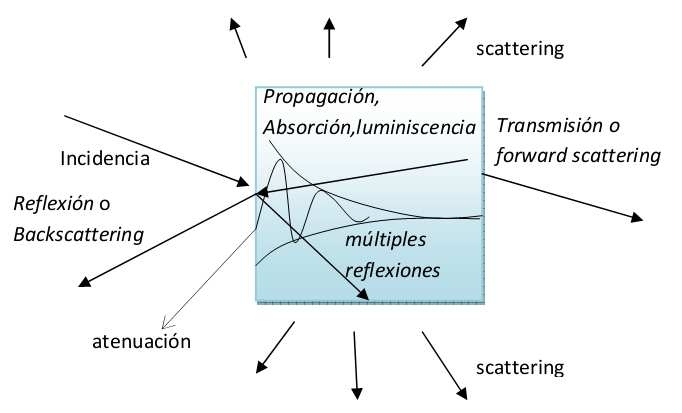
\includegraphics[scale=.3]{../Images/ep1}
	\caption{\emph{Esquema de los procesos de dispersión de luz por un objeto infinito o semiinfinito general}}
	\label{fig:CP11}
\end{figure}
De manera que, no hay modos de luz que puedan propagarse si tienen una frecuencia dentro de dicho rango. Un espejo dieléctrico simple no puede tener un gap fotónico completo, porque las dispersiones ocurren solo a lo largo de un eje. En relación para crear un material con un gap fotónico completo, debemos fijar el contraste dieléctrico en una red que es periódica a lo largo de tres ejes.
Algunas de las características que describen a determinados cristales fotónicos son el aumento local del campo, la dispersión anómala de la velocidad del grupo, y la dispersión anómala en el índice de refracciones puede construir una amplia variedad de CFS son diferentes materiales dieléctricos {8,58}. Además, dependiendo de los materiales seleccionados para diseñar los CFS, es posible fabricar estructuras fotónicas con periodicidad dieléctrica en una dimensión (1D), dos dimensiones (2D), y tres dimensiones (3D) , donde es posible sintonizar las bandas prohibidas en diferentes regiones del espectro electromagnético si los grosores finales de las capas que constituyen las estructuras se seleccionan adecuadamente    



\subsection{ Comparación entre cristales sólidos (CS) y cristales fotónicos (CF)}

\begin{table}[H]
	\centering
	\begin{tabular}{| m{4cm} | m{4cm} | m{4cm} |}
		\hline 
		\textbf{CARACTERÍSTICA} & \textbf{CS} & \textbf{CF} \\ 
		\hline 
		\textbf{Función} & Función de Onda & Campo vectorial Electromagnético \\ 
		\hline 
		\textbf{Periodicidad} & Potencial & Constante dieléctricas \\ 
		\hline 
		\textbf{Función principal} & Concentran regiones de baja potencial &  
		Los campos se concentran su energía  eléctrica en regiones de alta constate dieléctrica \\ 
		\hline 
		\textbf{Bandas} & Conducción y Valencia & Las bandas superior e inferior al gap son la banda de aire y la dieléctrica. \\ 
		\hline 
		\textbf{Estructuras de bandas} & Nos dan las energías de los auto estados permitidos & La dispersión coherente de los campos electromagnéticos en interfaces entre regiones distintas constantes dieléctricas \\ 
		\hline 
		\textbf{Origen Bandas} & La dispersión coherente de la onda electrónica al atravesar regiones con diferente potencial & La dispersión coherente de los campos electromagnéticos en las interfaces de distintas constante dieléctrica. \\ 
		\hline 
		\textbf{Defectos} & Puede crear un estado permitido en el interior del gap que posibilita la existencia de un estado electrónico localizado alrededor del defecto & Puede crear un estado en ele interior del gap que posibilita la existencia de un modo localizado del defecto. \\ 
		\hline 
	\end{tabular} 
	\caption{ \emph{Tenemos  diferentes puntos denotado de la siguiente forma,  }}
	\label{tabla:01}
\end{table}
%++++++++++++++++++++++++++
\section{ Materiales dieléctricos porosos}

Recientemente los materiales porosos han llamado la atención por sus usos en varias áreas tales como la química, ingeniería química, investigación de semiconductores, y el desarrollo de sensores físicos, químicos y biológicos. Otra aplicación que se le ha dado a los materiales porosos es para el crecimiento cristalino. Existen diferentes materiales porosos con los cuales se pueden construir diversos sistemas de multicapas dieléctricas. Por ejemplo, la alúmina porosa (AP) es un material usado para fabricación de cristales fotónicos debido su bajo coeficiente de absorción en la región visible e infrarroja. . Otro material ampliamente usado debido  a que presenta una fotoluminiscencia eficiente a temperatura es el SP, el con el cual también es posible fabricar cristales fotónicos en 1D, 2D Y 3D. Por lo que nos enfocaremos con más detalle al silicio  en su forma porosa.
\subsection{ Silicio cristalino}
El silicio (si) es uno de los elementos más abundantes en la corteza con 27 \% en peso después del oxígeno. Este elemento se presenta en forma amorfa y cristalina. El si es empleado ampliamente en dispositivos electrónicos y en la fabricación de celdas solares. Sin embargo este elemento no tiene buenas propiedades ópticas, ya que posee una banda de energía prohibida indirecta de aproximadamente  motivo por el cual, este material no emite radiación eficientemente aun a bajas temperaturas. El movimiento de un electrón hacia la banda de conducción y su regreso a la banda de valencia (recombinación par electrón y hueco), requiere de los fonones, para que el momento se conserve, este tipo de transición radiactiva es generalmente muy ineficiente desde el punto de vista óptico .
\subsection{Formación de silicio poroso}
El SiP es obtenido por el ataque oxidativo electroquímico al silicio cristalino. Una de las principales ventajas de trabajar con silicio poroso es que es muy sencillo y rápido de obtener. Para su fabricación no se requiere de un equipo muy sofisticado y costoso. Sin embargo, las aplicaciones de esta materia en el ámbito tecnológico y científico son muy diversas. Para su fabricación existen varias técnicas tales como stain etching y spark ersion. Stain etchig es útil para producir SP sobre sustratos que no tienen que no tiene una buena conductividad (baja concentración de dopaje), mientras que spark erosion tien la única ventaja de que es un proceso totalmente en seco. Sin embargo, la técnica más común para fabricación de SP consiste de un proceso electroquímico denominada anodización electroquímica. Este proceso fue utilizado por primera vez por Uhlir\cite{I101}, y con él se pueden obtener capas gruesas y muy homogéneas. Además la anodización electroquímica permite controlar la velocidad de ataque elctroquimico, con lo cual se puede tener un control preciso de las propiedades de las películas tales como el espesor y la porosidad. La formación de SP mediante anodización consiste en la disolución electroquímica de silicio cristalino en una solución acuosa o etanolica de ácido fluorhídrico (HF), el proceso de anodización puede realizarse en modo de voltaje controlado a modo de corriente controlada. Sin embargo, el ultimo es el que se usa normalmente ya que proporciona un control mucho mejor en la porosidad y en el espesor de las capas, así como también proporciona una buena reproducción entre muestras. En la fabricación del SP todos los factores experimentales son importantes tales como: el tipo de conductividad de las obleas (n o p), su nivel de dopaje, composición del electrolito (Ph, concentración), construcción de la celda electrolítica, el régimen de anodización, la preparación previa de la muestra, etc. Muy recientemente una nueva técnica parta la obtención de SP a partir de obleas por efecto Hall ha sido realizada. En esta técnica se sustituye el efecto de la luz UV  del método tradicional por un c campo magnético. Un gradiente lateral puede ser logrado usando campo magnético, además de alterar la nanoestructura del SP.

\subsection{Celda usada para la anodización electroquímica convencionalmente} 
Se han propuesto diversos tipos de celda para realizar el proceso de anodización \cite{109}.  

\begin{figure}[H]
	\centering
	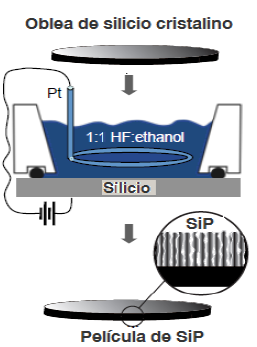
\includegraphics[scale=.7]{../Images/esp}
	\caption{\emph{Esquemático de una celda electroquímica de dos electrodos utilizada para fabricar SiP. La oblea de Si (ánodo) es el electrodo de trabajo y en su superficie ocurre una reacción de oxidación/disolución.}}
	\label{fig:CP13}
\end{figure}
la figura \textbf{\ref{fig:CP13}} muestra la celda más usada para fabricar  SiP, conocida como celda de tanque, usa un contacto (una lamina  de un material  conductor)  en la parte posterior  de la oblea. En este tipo de celda se requiere que haya un buen contacto entre la oblea de Si y la lámina de metal. Por lo tanto, un contacto metálico (por lo general de Al) es depositado  sobre la parte posterior  de la oblea de silicio y sellado a fin de que sólo la parte frontal de la muestra (lado pulido  de la oblea) sea expuesta  al electrólito  de anodización.  En una oblea de silicio  con una baja resistividad (típicamente menor que $1 mcm$) se obtiene una buena uniformidad sin la necesidad de depositar un contacto metálico. 
Sin embargo, para obleas de silicio de alta resistividad  (típicamente mayor que 1 cm), se requiere la implantación de una alta dosis de boro (tipo p) o fósforo (tipo n) sobre el lado no pulido de la oblea para una buena uniformidad.  Con este tipo de celda se obtienen capas de SP con una buena uniformidad, simplificandose la interpretación  de las características de corriente-voltaje (i-V), y ofreciendo un buen control del espesor y la porosidad, que son claves en la fabricación de CFs con muy buena calidad óptica.


La posibilidad de formar estructuras con monocapas y multicapas a base de silicio poroso mediante el método de anodización electroquímica es relativamente simple. Para la formación de diferentes capas la influencia de los parámetros de ataque son cruciales, ya que si requerimos de una capa porosa con un determinado tamaño promedio del poro debemos usar una determinada resistividad y un determinado tipo de obleas, así como también una concentración especifica de ácido fluorhídrico (HF), existe básicamente dos tipos de multicapas de SP . En el primer tipo de multicapas, la densidad de corriente se examina durante la anodización.
\subsection{Características Corriente-Voltaje (I-V)}
\begin{figure}[H]
	\centering
	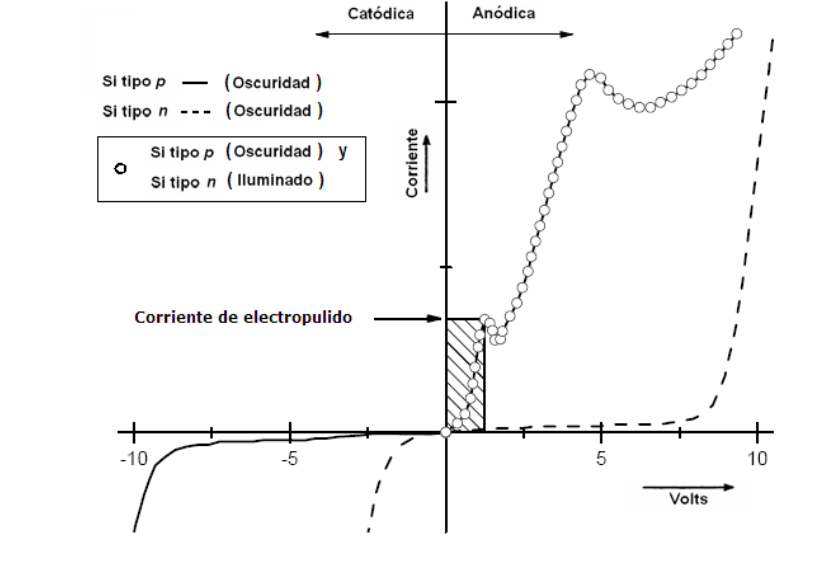
\includegraphics[scale=.55]{../Images/iv}
	\caption{\emph{Representacion de las características típicas de corriente-voltaje (i-V) en el proceso de anodización para
			silicio tipo n y tipo p en solución acuosa de HF. La región dentro del rectángulo corresponde al régimen útil donde se puede lograr el SiP,
			asumiendo la curva característica i-V marcada con círculos vacíos. En el régimen anódico, las características de una celda electroquímica con silicio tipo n estarán en la región delimitada por las características en obscuridad (linea punteada) y con iluminación (círculos vacíos)\cite{110}.}}
	\label{fig:iv}
\end{figure}
En la Figura \textbf{\ref{fig:iv}} se muestran Las características típicas de corriente-voltaje (i-V) en el proceso de anodización para silicio tipo n y tipo p en solución acuosa de HF se muestran\cite{110}. Se debe poner énfasis en que la cantidad física que se mide es la densidad de corriente
J (en la interfase silicio/electrólito), en lugar de la corriente absoluta i. Para formar el SP la corriente en el lado del silicio de la interfase silicio/electrólito debe ser generada por los huecos inyectados desde el sustrato (bulto de silicio) hacia la interfase. La corriente debe estar entre cero y el umbral de electropulido, el cual se identifica como el valor del primer máximo del régimen anódico en la curva (i-V). Los regímenes útiles son incluidos en la región marcada con un rectángulo en la  Figura \textbf{\ref{fig:iv}}, donde el voltaje en el umbral de electropulido (para la curva marcada con círculos vacíos) es $V \equiv 1.3V$ . Los valores cuantitativos de las curvas i-V, así como los valores correspondientes al pico de electropulido dependen de los parámetros de ataque y del nivel de impurezas de la oblea. En el caso de silicio tipo n se requiere de iluminación externa para lograr una corriente significante de huecos dependiendo del nivel de dopaje. Si la corriente excede el umbral de electropulido la anodización resulta en un removimiento progresivo y completo del silicio, esto es, la oblea tiene entonces una apariencia como la de un espejo.
\subsection{Química de formación del SiP}
El mecanismo de la  disolución química de Si es aún un tema en discusión y se han propuesto diferentes modelos para tratar de explicarlo. Sin embargo, generalmente se acepta que es necesaria la presencia de los huecos para la formación de los poros y para el proceso de electropulido \cite{110, 112}. Cuando se lleva a cabo la formación del poro, dos átomos de hidrógeno se desprenden por cada átomo de Si disuelto [113]. El desprendimiento de hidrógeno disminuye cuando el proceso se aproxima al régimen de electropulido y desaparece durante el electropulido. La eficiencia de la corriente es de alrededor de dos electrones por cada átomo de Si disuelto durante la formación del poro y de alrededor de cuatro electrones en el régimen de electropulido \cite{112}.
\begin{figure}[H]
	\centering
	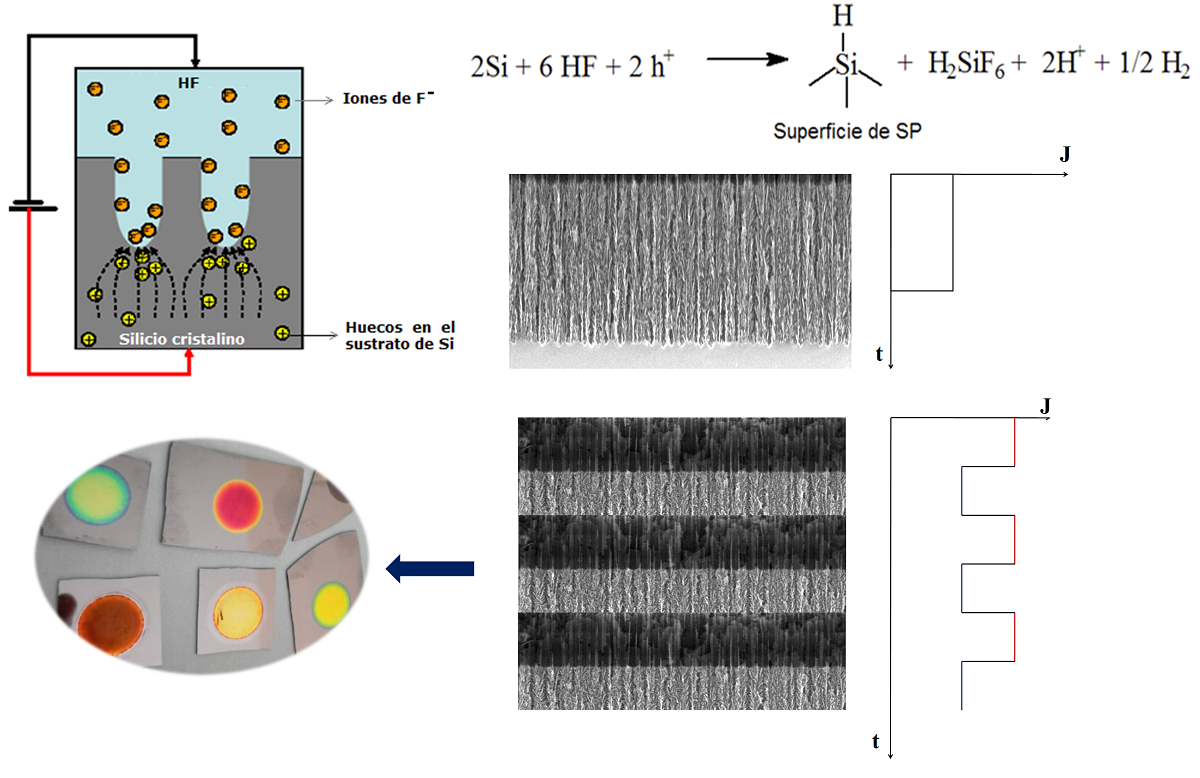
\includegraphics[scale=.4]{../Images/spfor}
	\caption{\emph{Esquema  del proceso electroquímico de anodización del Si cristalino utilizando
			un proceso con densidades corriente controlada. Los iones $F^-$ (contenidos en la solución electrolítica)
			y los huecos (presentes en la oblea de Si) son las principales especies electroactivas que intervienen
			en el proceso de anodización, esto es, el ataque ocurre solo en las puntas del poro donde los huecos
			($h^+$) son enfocados por el campo eléctrico \cite{114}.}}
	\label{fig:Qf}
\end{figure}
La Figura \textbf{\ref{fig:CP14}} nos muestra el esquema  del proceso electroquímico de anodización del Si cristalino utilizando
un proceso con densidades corriente controlada. Los iones $F^-$ (contenidos en la solución electrolítica) y los huecos (presentes en la oblea de Si) son las principales especies electroactivas que intervienen en el proceso de anodización, esto es, el ataque ocurre solo en las puntas del poro donde los huecos ($h^+$) son enfocados por el campo eléctrico \cite{114}. 

\begin{figure}[H]
	\centering
	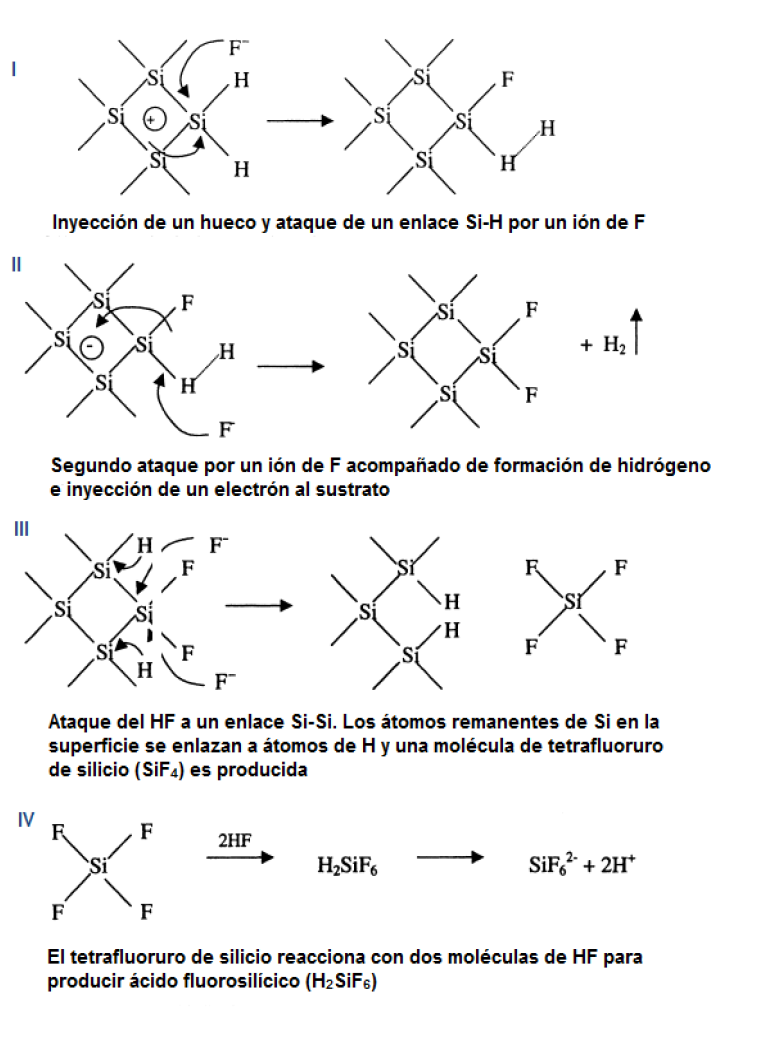
\includegraphics[scale=.55]{../Images/hf}
	\caption{\emph{Mecanismo de formación de poros por disolución electroquímica en electrólitos de HF.}}
	\label{fig:CP14}
\end{figure}
 La Figura \textbf{\ref{fig:CP14}} ilustra el mecanismo de la disolución química que fue sugerido por Lehmann y Gosele en 1991, el cual esta basado en un esquema de oxidación de los enlaces superficiales con captura de huecos y una subsiguiente inyección electrones, los cuales inducen estados de oxidación divalentes. El proceso de disolución de Si en HF se describe brevemente en los pasos (1 al 5) del esquema de Figura \textbf{\ref{fig:CP14}}.

\subsection{Porosidad}
La porosidad es el parámetro mas importante cuando caracterizamos un material poroso, la cual se define como la razón del volumen ocupado por el poro con respecto al volumen total. La porosidad de una muestra de SP puede ser calculada por gravimetría usando la siguiente ecuación 
\begin{equation}
P= \bigg(  \frac{m_1-m_2}{m_1 -m_3} \bigg) 
\end{equation}
donde $m_1$ es la masa en gramos de la oblea de silicio inicial, $m_2$ es la masa de la oblea de silicio después de la anodización, en gramos, $m_3$ es la masa del silicio después de la disolución de la capa porosa, en gramos, y P es la porosidad en porcentaje. Se muestra un esquema simplificado de estas masas que intervienen en el método gravimétrico. Es importante señalar que para remover la capa porosa
en $m_2$ , se usa una solución de hidróxido de sodio (1 molar) o se realiza un electropulido sobre la capa porosa. El método gravimétrico es aplicable
en los casos donde la capa de SP es suficientemente gruesa $(> 5 \ \ \mu m)$. La diferencia en masa es más grande que la cantidad de error inducido en las mediciones. Sin embargo, cuando la capa de SP es delgada $(< 200 \ \ nm)$, la diferencia en masa es del
mismo orden de magnitud que el error en las mediciones y el valor de la porosidad.
\begin{figure}[H]
	\centering
	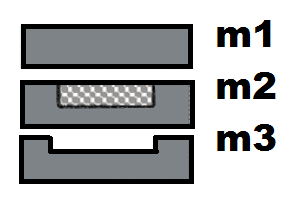
\includegraphics[scale=.5]{../Images/poros}
	\caption{\emph{Esquema de las masas que intervienen en el cálculo de la porosidad.}}
	\label{fig:CP15}
\end{figure}

\subsection{Espesor}
El espesor de una capa de silicio poroso puede ser obtenido usando un perfilómetro. Las películas con espesores de la capa del orden de micras pueden ser medidas muy fácilmente, sin embargo, cuando las capas son muy delgadas (por ejemplo 80 nm) los espesores medidos no son muy confiables. Un método alternativo consiste en obtener el espesor de una forma indirecta utilizando mediciones gravimétricas, mediante la siguiente relación 
\begin{equation}
d= \bigg(\frac{m_1-m_3}{\rho_Si S}\bigg)
\end{equation}
donde $\rho$ es la densidad del silicio y S es la superficie atacada. Sin embargo, para obtener valores mas precisos del espesor de las capas, se puede recurrir a la medición del espesor de la capa directamente desde una imagen de sección transversal de SEM. Mediante ésta técnica se puede obtener información muy útil acerca del perfil y del tipo de rugosidad presente en la interfase SP/Si, con lo cual se puede tener un valor
cuantitativo sobre la homogeneidad de la capa de SP.
\subsection{Índice de refracción}
Para las aplicaciones ópticas de los materiales multicapas (espejos de Bragg, espejos omnidireccionales y microcavidades), es necesario conocer el índice de refracción de cada capa del material constituyente. Un método muy simple para evaluar el índice de refracción de un material tipo película (monocapa), consiste en la medición de las franjas de interferencia de las reflexiones múltiples de un haz de luz al propagarse a través de la película a diferentes longitudes de onda , a fin de obtener el espesor óptico del haz de luz . La posición de la franja de interferencia máxima satisface: $2nd \bigg(\frac{1}{\lambda_r}-\frac{1}{\lambda_{r+1}} \bigg)=1$, donde n es el índice de refracción, d es el espesor de la capa y $\lambda_r$ es la longitud de onda correspondiente al r-ésimo máximo de reflectancia. Si el espesor de la capa es conocido independientemente (por SEM o gravimetría), el índice de refracción se obtiene fácilmente de la ecuación mediante la razón entre el camino óptico nd y el espesor de la capa. Este método puede utilizarse solamente si las franjas de interferencia son visibles y si la capa es delgada. Si el material presenta una gran dispersión, otros métodos deberán de ser empleados. Con frecuencia, se emplea la técnica de elipsometría para obtener los valores de n y k, para un amplio rango de frecuencias . Los índices de refracción correspondientes a las diferentes capas porosas con las que fabricamos nuestras estructuras son obtenidos usando un método de aproximación del medio efectivo.
\subsection{Anodización Asimétrica }
\begin{figure}[H]
	\centering
	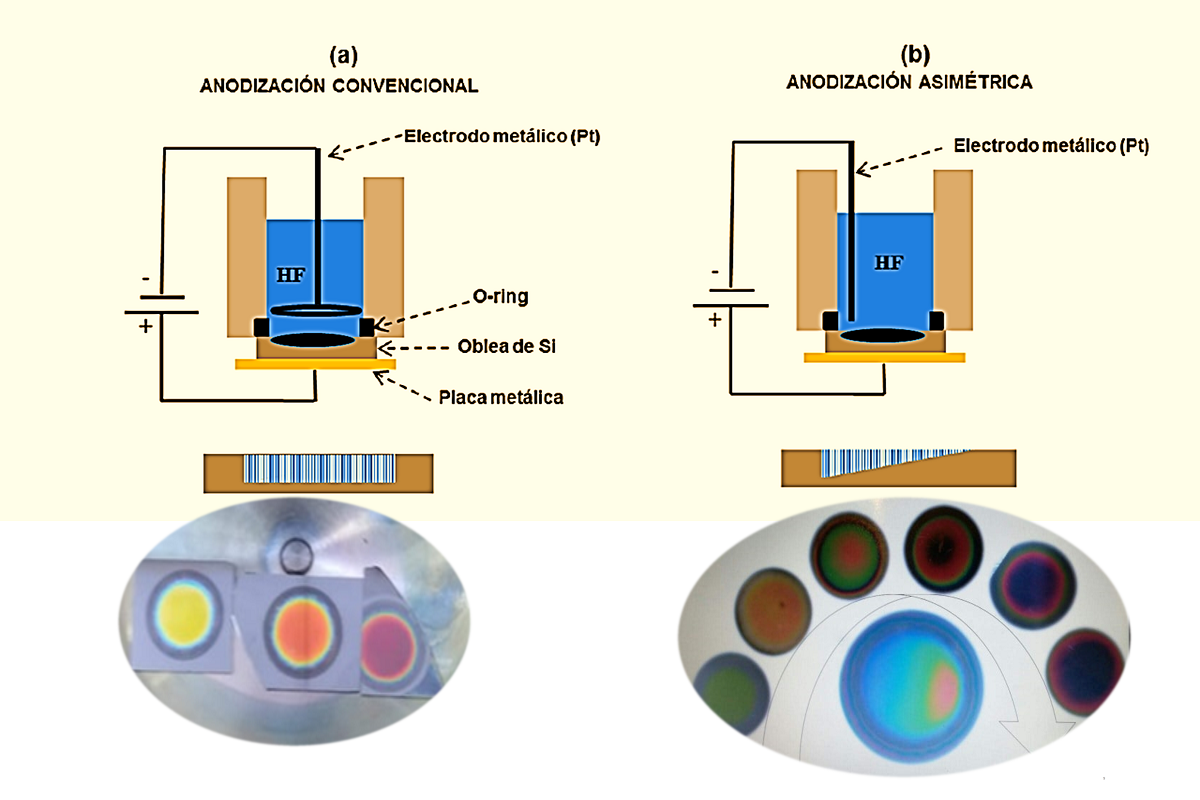
\includegraphics[scale=.4]{../Images/an}
	\caption{\emph{(a) Anodización convencional. La muestra es atacada uniformemente lo que resulta en una muestra con espesor constante (b) Anodización asimétrica resultando en muestras con un gradiente en espesor y tamaños de poros.}}
	\label{fig:CPAA}
\end{figure}
En la fabricación convencional de SiP el resultado deseado es obtener muestras homogéneas (mismas características estructurales) desde la periferia hasta el centro del área atacada electroquímicamente \textbf{Figura \ref{fig:CPAA} a)}. Sin embargo, con una configuración de anodización asimétrica se obtienen muestras con un gradiente lateral en términos de tamaño de poro y espesor de la capa porosa. En esta configuración, la cara del electrodo de platino (cátodo) se mantiene relativamente perpendicular a la superficie del sustrato de Si (ánodo) en uno de los extremos de la celda como se muestra en la Figura \textbf{\ref{fig:CPAA} b)}, de tal forma que la distribución de la corriente dentro de la solución electrolítica varía en función de la distancia del electrodo debido a la resistencia del electrolito, resultando en una disminución de la densidad de corriente conforme la distancia desde el electrodo aumenta. El resultado es una superficie porosa con diferentes tamaños de poros que van desde unos cuantos nanómetros hasta poros del orden de unos cuantos micrómetros. Las dimensiones de los poros obtenidos en el mismo chip pueden controlarse ajustando la corriente de anodización y la concentración del electrolito .


\subsection{El ancho completo a la mitad del máximo(FWHM)}
\begin{figure}[H]
	\centering
	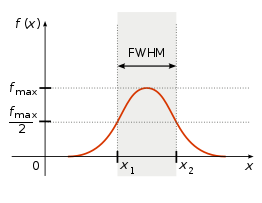
\includegraphics[scale=1]{../Images/fwhm}
	\caption{\emph{Esquema del ancho completo a la mitad del ancho de banda máximo (FWHM) para una curva de resonancia. El eje horizontal es frecuencia, el eje vertical es amplitud. El FWHM es el ancho en frecuencia de la región sombreada entre los puntos de la curva donde la amplitud se ha reducido a la mitad de la amplitud máxima. Las etiquetas variables en este dibujo pueden haberse cambiado accidentalmente, porque los valores de amplitud en el eje vertical están etiquetados como $f_{max}$ , mientras que los valores de frecuencia en el eje horizontal están etiquetados $x_1$ y $x_2$ .}}
\end{figure}
En la Figura El ancho completo a la mitad del máximo ( En ingles Full width at half maximum (FWHM) ) es una expresión de la extensión de la función dada por la diferencia entre los dos valores extremos de la variable independiente en la que la variable dependiente es igual a la mitad de su valor máximo. En otras palabras, es el ancho de una curva espectral medida entre esos puntos en el eje y que son la mitad de la amplitud máxima. FWHM se aplica a fenómenos tales como la duración de las formas de onda del pulso y el ancho espectral de las fuentes utilizadas para las comunicaciones ópticas y la resolución de los espectrómetros. El término duración completa a la mitad máximo (FDHM) se prefiere cuando la variable independiente es el tiempo. La convención de ancho que significa "medio máximo" también se usa ampliamente en el procesamiento de señal para definir ancho de banda como ancho de rango de frecuencia donde menos de la mitad de la potencia de la señal se atenúa, es decir, la potencia es al menos la mitad del máximo. En términos de procesamiento de señales, esto es como máximo de de atenuación, llamado " punto de media potencia "

%++++++++++++++++++++++++++
\section{Propiedades Silicio Poroso}
\begin{figure}[H]
\centering
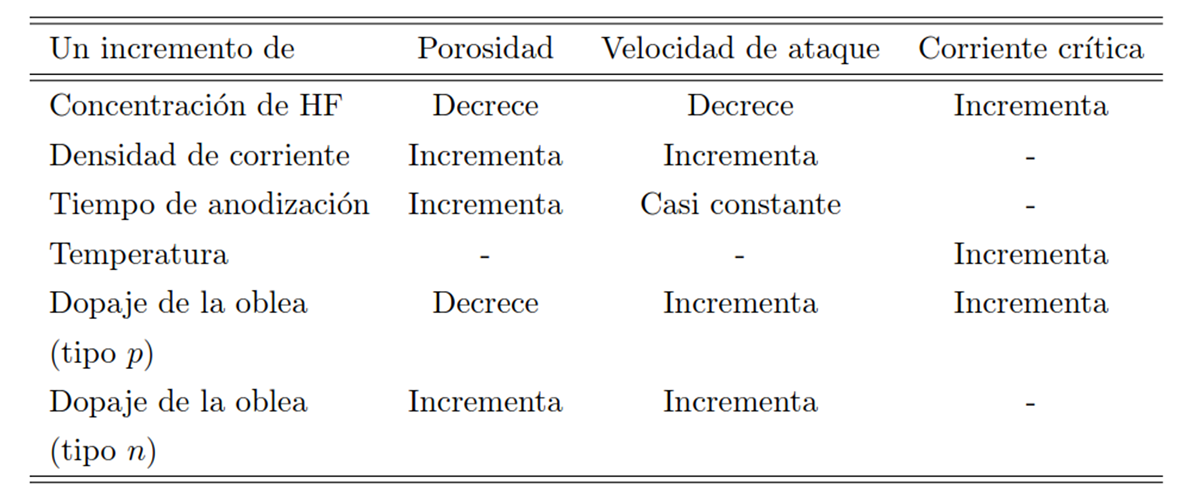
\includegraphics[scale=.4]{../Images/pp1}
\caption{\emph{Efecto de los parámetros de anodización sobre la formación del SiP [101].}}
\label{fig:pp1}
\end{figure}
\begin{figure}[H]
	\centering
	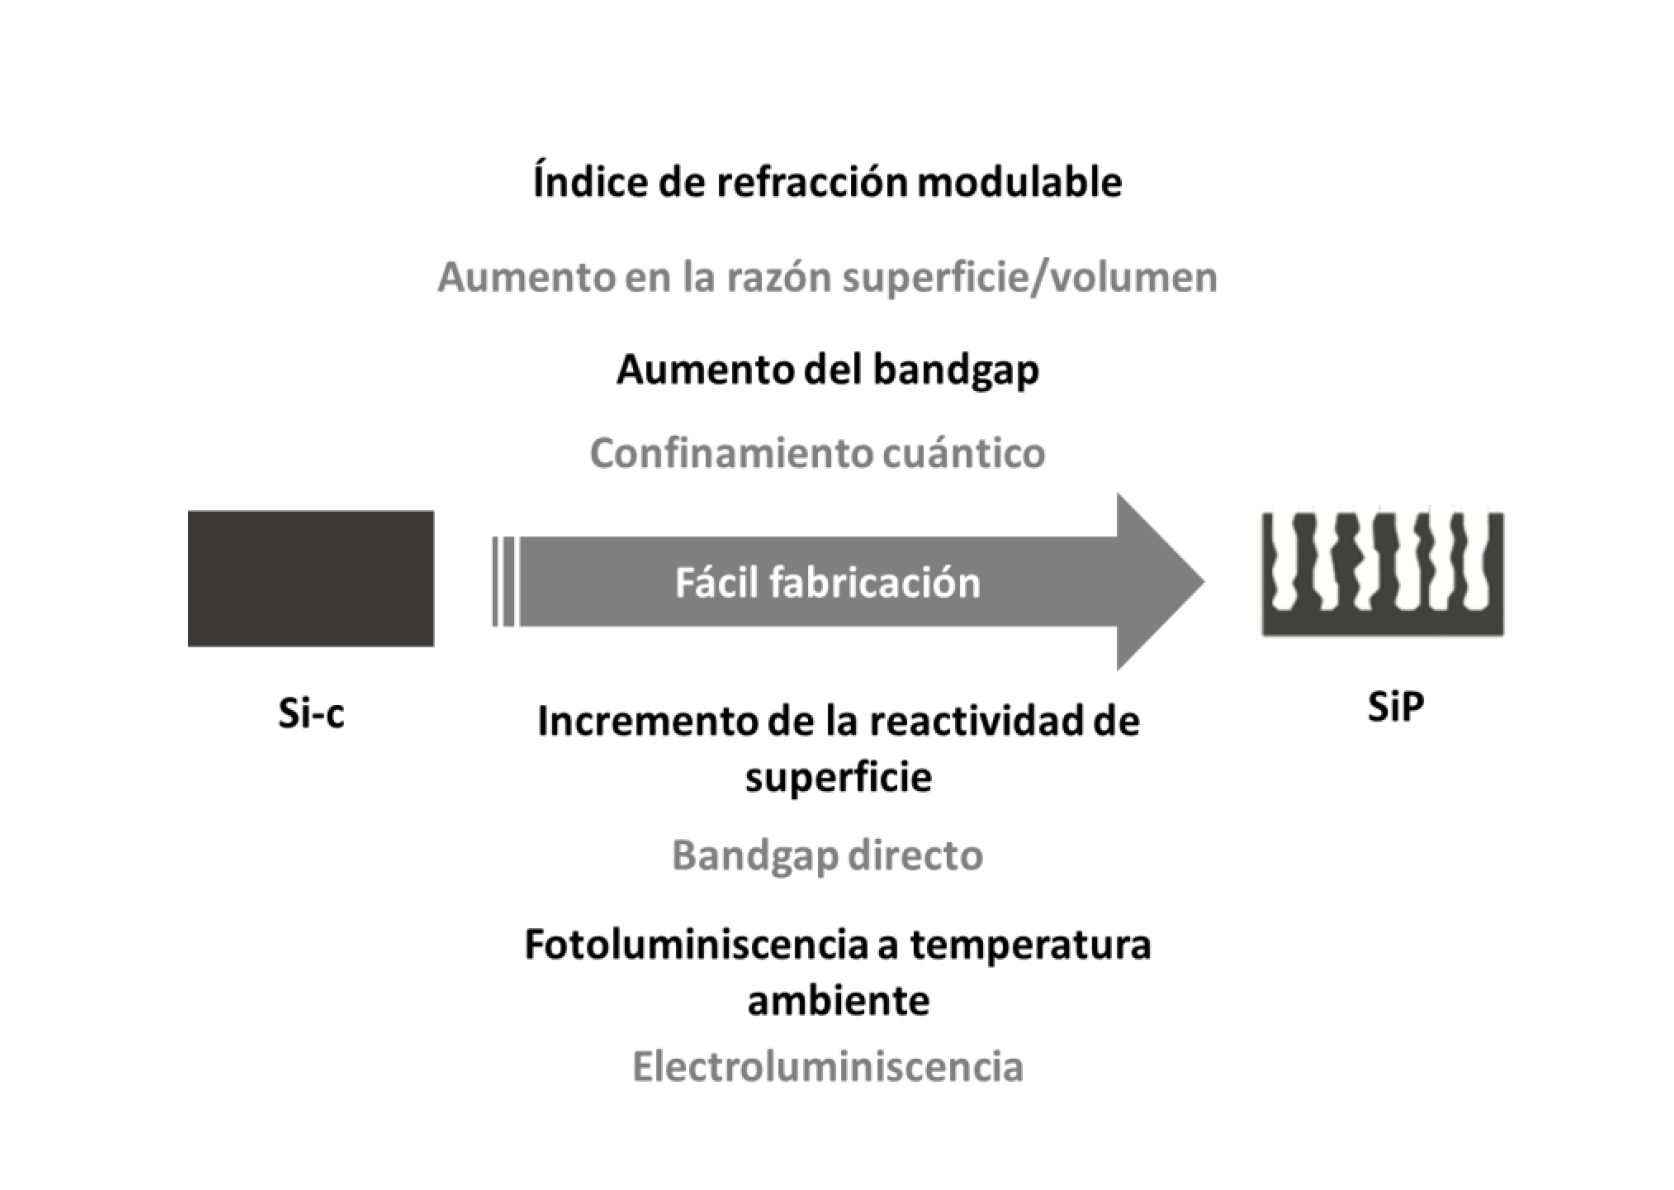
\includegraphics[scale=.3]{../Images/sil}
	\caption{\emph{Cambio en las propiedades del Si cristalino al convertirlo a SiP}}
	\label{fig:CP12}
\end{figure}

\begin{figure}[H]
	\centering
	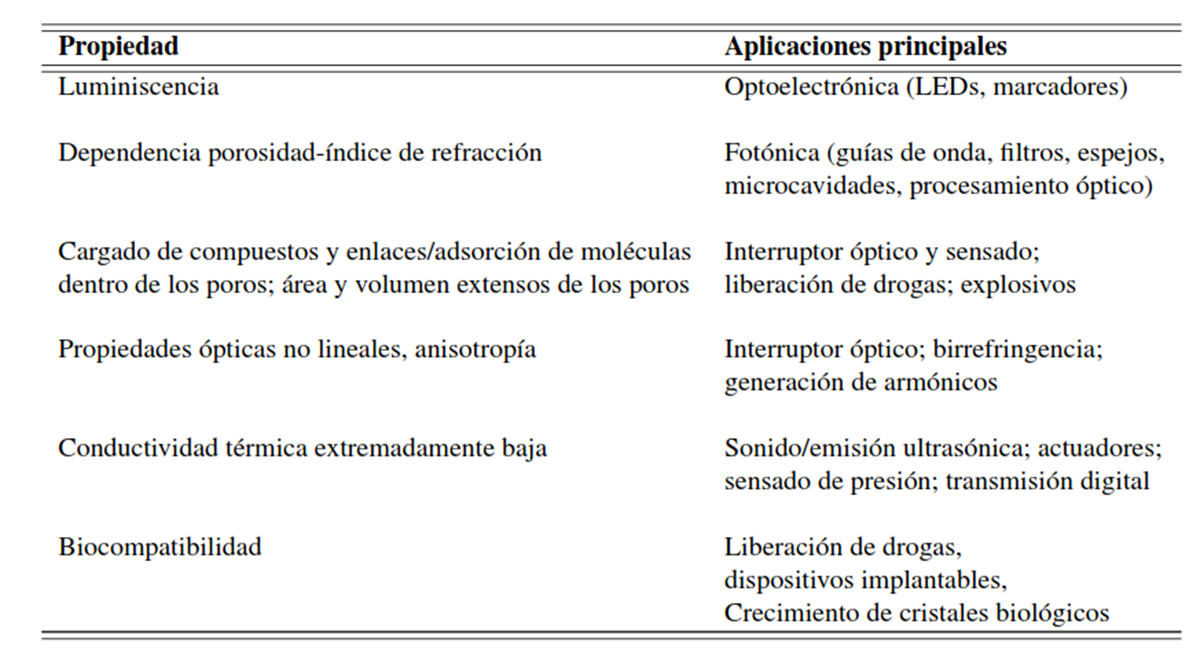
\includegraphics[scale=.4]{../Images/propiedades}
	\caption{\emph{Una tabla que muestra las propiedades del SiP}}
	\label{fig:prp}
\end{figure}
\section{Sistemas Ordenados}
En todas las ramas de la ciencia es muy útil contar con un modelo teórico que describa algún fenómeno en particular. Ya sea que el modelo se utilice para ajustar datos después de realizado un experimento o que se le emplee para predecir un resultado, antes de poderlo comparar con los datos medidos, es necesario verificar que el método de cálculo sea estable numéricamente. De lo contrario, si no se tiene certeza numérica se producirán errores que solo son atribuibles al cómputo y no a la teoría en sí. Como se verá en esta tesis, este análisis es fundamental para el modelo de la matriz de transferencia\cite{1}. El método de matriz de transferencia se utiliza para resolver problemas físicos en sistemas que pueden dividirse en varias regiones o capas con fronteras bien definidas. Debido a esta generalidad se le encuentra en muchos campos de la ciencia y la ingeniería, en sismología por ejemplo se le utiliza para modelar las capas de la tierra, en mecánica cuántica para representar pozos y barreras del potencial, en electromagnetismo para describir el paso de la luz a través de una multicapa, etc \cite{2,3,4,5}. Lo que esta técnica permite es determinar como cambian las variables del problema al pasar de una región a otra, especialmente en las fronteras, donde el cambio de medios produce efectos importantes en estas. Lo que comúnmente se logra con este método es calcular los coeficientes de reflexión y transmisión o la relación de dispersión de toda una estructura.La forma más directa de obtener la matriz de transferencia consiste en asociar a cada región o capa una matriz individual, con la multiplicación de todas estas, se obtiene una matriz para toda la estructura y con sus elementos pueden conocerse las cantidades mencionadas anteriormente\cite{6,7,8,9,10,11}
\subsection{Matriz de transferencia}
Para un sistema de un material, el comportamiento electrónico puede darse por una estructura de bandas de los niveles electrónicos que corresponden a una energía determinada que tienen en cuenta todas las propiedades ópticas y eléctricas del material.
Las propiedades  óptica de un cristal fotónico (CF) están directamente relacionadas a su relación de dispersión.
Para el análisis teórico de los CFs se considera una estructura 1D que consiste de capas alternantes de SP de diferentes  índices de refracción acopladas a un medio homogéneo en la interfase, caracterizado por un índice de refracción $n_{_{0}}$. La bandas fotónica omnidireccional y el espectro de reflectividad de la estructura de multicapas se estudian por el método de la matriz de transferencia. La estructura dieléctrica está definida por:
\begin{equation}
%\[
n(z)= \left\{ \begin{array}{lcl}
n_{_{0}}& \mbox{ , } & z<z_{_{0}} \\
n_{_{1}}& \mbox{ , } & z_{_{0}}<z<z_{_{1}}  \mbox{con} \ \ \ \ z_{_{1}}=z_{_{0}}+h_{_{1}} \\
n_{_{2}}& \mbox{ , } & z_{_{1}}<z<z_{_{2}}  \mbox{con} \ \ \ \ z_{_{2}}= z_{_{0}}+\Lambda=z_{_{1}}+h_{_{2}} \\
\vdots \\
n_{_{s}} & \mbox{,} & z_{_{2N}}<z \ \ \mbox{ con } \ \ z_{_{2N}}=z_{_{0}}+N\Lambda=z_{_{2N-1}}+h_{_{2}}
\end{array}
\right.
%\]
\end{equation}
con $ n_{_{z}}=n(z+\Lambda) $, siendo $ n_{_{s}}$ es el índice de refracción del sustrato y $ n_{_{i}}$ $(i=0,1,2...)$, el índice de refracción del medio incidente, y los espesores de las capas están relacionada en $ z_{_{m}}$ y $ h_{_{m}}$  \\
Para el caso descrito, la onda electromagnética incide sobre la interface de separación haciendo un ángulo $ \theta_{_{m}} $ con respecto a la normal. Por lo tanto, es posible
descomponer la onda con respecto al plano de incidencia $XZ$ en una componente perpendicular TE (transversal eléctrica) y en una componente paralela
TM (transversal magnética). El vector de onda incidente tiene componentes
en $X $ y $Z$, $k_{_{m}}=(k_{_{mx}},0,k_{_{mz}})$ es decir:
\begin{equation}
k_{_{m}}= \frac{\omega}{c} \bigg(n_{_{m}}k_{_{mx}} \sin (\theta_{_{m}}),0,n_{_{m}}k_{_{mz}} \cos( \theta_{_{m}}) \bigg) \
\end{equation}
Como se supone que los medios son homogéneos en $X$, los índices de refracción no varían en esa
dirección $n(z)$, el módulo del campo eléctrico es:
\begin{equation}
E(x,z,t)=E(z)e^{i(\omega t-k_{_{mx}} x)}
\end{equation}

\begin{figure}[H]
	\centering
	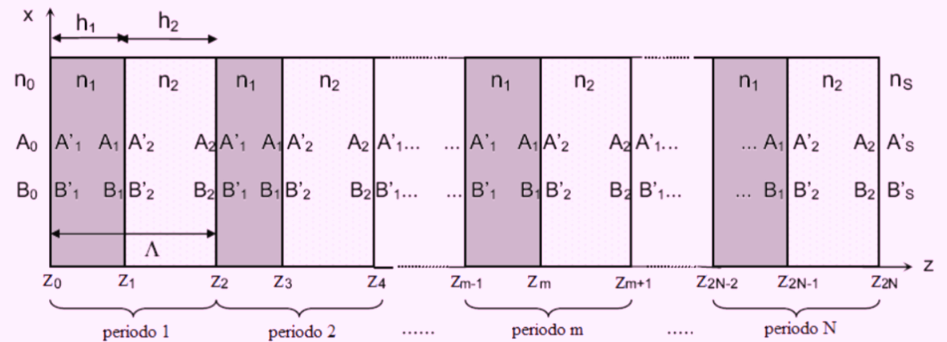
\includegraphics[scale=.45]{../Images/MTT}
	\caption{\emph{Diagrama de} }
	\label{fig:MTT}
\end{figure}

La ecuación (3) es válida tanto si con respecto al plano de incidencia, el campo eléctrico es perpendicular o si está contenido en él. A medida que la onda electromagnética avanza a lo largo de la estructura, experimenta múltiples reflexiones en cada una de las interfaces. En este caso $E(z)$, está constituido por la onda que viaja a la derecha $(+Z)$ y otra a la izquierda $(-Z)$:

\begin{equation}
%\[
E(z)= \left\{ \begin{array}{lcl}
A_{_{0}}e^{-ik_{_{0z}}(z-z_{_{0}})}+ B_{_{0}}e^{-ik_{_{0z}}(z-z_{_{0}})}  \ \ \ \ \ \ z<z_{_{0}}  \\
A_{_{m}}e^{-ik_{_{mz}}(z-z_{_{m}})}+ B_{_{m}}e^{-ik_{_{mz}}(z-z_{_{m}})}  \ \ \ \ \ \ z_{_{m-1}}<z<z_{_{m}}  \\

A^{'}_{_{s}}e^{-ik_{_{sz}}(z-z_{_{2N}})}+ B^{'}_{_{s}}e^{-ik_{_{sz}}(z-z_{_{2N}})}  \ \ \ \ \ \ z_{_{2N}}<z

\end{array}
\right.
%\]
\end{equation}


donde $k_{_{mz}}$ es la componente $z$ del vector de onda $k_{_{mz}}=\omega n_{_{n}} \cos \theta_{_{m}}/c$ y $ \theta_{_{m}} $ es el ángulo entre la dirección de propagación y el eje $ z $. $A_{_{m}}$ y $B_{_{m}}$ representan las amplitudes de las ondas en la interfases $z=z_{_{mz}}$

Las amplitudes de las ondas en las diferentes capas pueden relacionarse por:
\begin{equation}
{A_{_{m-1}} \choose B_{_{m-1}}} = D^{-1}_{_{m-1}}D_{_{m}}{A^{'}_{_{m}} \choose B^{'}_{_{m}}} = D^{-1}_{_{m-1}}D_{_{m}}P_{_{m}}{A_{_{m}} \choose B_{_{m}}}
\end{equation}
Para $m=1,2,...2N+1;$ donde la matriz D(matriz dinámica) y P(matriz de propagación) se puede escribir como:
Para la onda TE
\begin{equation}
D_{_{m}} = \left( \begin{array}{lcccl}
1 & 1\\

n_{_{m}}\cos \theta_{_{m}} & -n_{_{m}}\cos \theta_{_{m}}

\end{array}
\right)
\end{equation}

La onda TM;
\begin{equation}
D_{_{m}} = \left( \begin{array}{lcccl}
\cos \theta_{_{m}} & \cos \theta_{_{m}}\\

n_{_{m}} & -n_{_{m}}

\end{array}
\right)
\end{equation}

Para las ondas TE y TM 
\begin{equation}
P_{_{m}} = \left( \begin{array}{lcccl}
e^{ik_{_{mz}}h_{_{m}}} & 0\\

0 & e^{-ik_{_{mz}}h_{_{m}}}

\end{array}
\right)
\end{equation}

La relación entre $ A_{_{0}}, B_{_{0}} $ y $ A^{'}_{_{s}}, B^{'}_{_{s}} $ se puede escribir como:
\begin{equation}
{A_{_{0}} \choose B_{_{0}}} = D^{-1}_{_{0}}(D_{_{1}} P_{_{1}}D^{-1}_{_{1}}D_{_{2}}P_{_{2}}D^{-1}_{_{2}})^{N}D_{_{s}}={M_{_{11}} \\  \ \ M_{_{12}} \choose M_{_{21}} \\ \ \ M_{_{23}} }{A^{'}_{_{s}} \choose B^{'}_{_{s}}}
\end{equation}
donde N es el número de periodos en la estructura. La reflectividad de la película de multicapas se calcula de los elementos de la matriz de la siguiente manera:
\begin{eqnarray}
R= \bigg \vert\frac{M_{_{12}}}{M_{_{11}}} \bigg \vert^{2}
\end{eqnarray}
Podemos obtener la relación de dispersión, para cada ángulo de incidencia para las polarizaciones TE y TM de la matriz característica de un periodo de la estructura:
\begin{equation}\label{Eq:m1}
{A_{_{0}} \choose B_{_{0}}}_{n-1} = D^{-1}_{_{1}}D_{_{2}} P_{_{2}}D^{-1}_{_{2}}D_{_{1}}P_{_{1}}{A_{_{1}} \choose B_{_{1}}}_{n}={S \\  \ \ T \choose U \\ \ \ V }{A_{_{1}} \choose B_{_{1}}}_{n}
\end{equation}
La ecuación \textbf{\ref{Eq:m1}} muestra la matriz característica de un periodo (dos capas) de la estructura con índices de refracción $n_{_{1}}$ y $n_{_{2}}$ . Las amplitudes se relacionan en el  $n-1$ con el periodo $n$. De acuerdo con el teorema de Floquet, las soluciones de las ecuaciones de onda para un medio periódico son de la forma
$E(z, x) = E_{_{K}}(z)e^{-i\beta x}e^{-iKz} $ donde $E_{_{K}}$ es periódico $E_{_{K}}(z + \Lambda) = E_{_{K}}$. La constante K es el número de onda de Bloch. Tomando en cuenta la forma de las matrices D y P es posible obtener la estructura de bandas a partir de los elementos de la matriz característica de la ecuación \textbf{\ref{Eq:m1}}, la cual se escribe como:
\begin{equation}\label{Eq:m2}
\cos K \Lambda = (S +V ) = \cos k_{1} d_{1} \cos k_{2} d_{2}-\phi \sin k_{1} d_{1} \sin k_{2} d_{2}
\end{equation}
donde $\phi=\frac{k_{_{2z}}}{k_{_{1z}}}+\frac{k_{_{1z}}}{k_{_{2z}}}$ para las ondas TE y $\phi=\frac{n^{2}_{_{2}}k_{_{1z}}}{n^{2}_{_{1}}k_{_{2z}}}+\frac{n^{2}_{_{1}}k_{_{2z}}}{n^{2}_{_{2}}k_{_{1z}}}$ para las ondas TM.
La relación de dispersión entre $\omega$, $\beta$, y $K$, donde $\beta=\omega n_{_{m}} \sin \theta/c$. Para observar la banda prohibida fotónica de las multicapas se calcula la relación de dispersión para todos los ángulos de incidencia, obteniendo la estructura de bandas proyectada. \\\\
\subsection{Teoría del medio efectivo}
La teoría del medio efectivo (TME) es u modelo físico que describe las propiedades macroscópicas de un medio, basado en las propiedades y fracciones de cada uno de sus componentes. Existen diversas aproximaciones para un medio efectivo, todas ellas asume que un sistema mascroscópico es homogéneo y el campo resultante en el sistema es un campo promedio de todas sus comoponentes.\\
El silicio poroso se puede represntar por la mexcla de dos materiales (aire y silicio) con constantes dieléctricas $\epsilon_1$ y $\epsilon_2$. Si la maezcla de estos dos materiales es lo suficientemente homogénea y el campo electromagnético externo no pueda distinguir la estructura de los campos del medio, entonces podemos suponer un medio efectivo. Así pues, supongamos un medio efectivo formado de pequeñas esferas dieléctricas (con constante dieléctrica $\epsilon_1$) inmesas en un medio dieléctrico (con constante dieléctrica $\epsilon_2$), como se muestra en la Fig. \textbf{\ref{fig:ME} a)}

\begin{figure}[H]
	\centering
	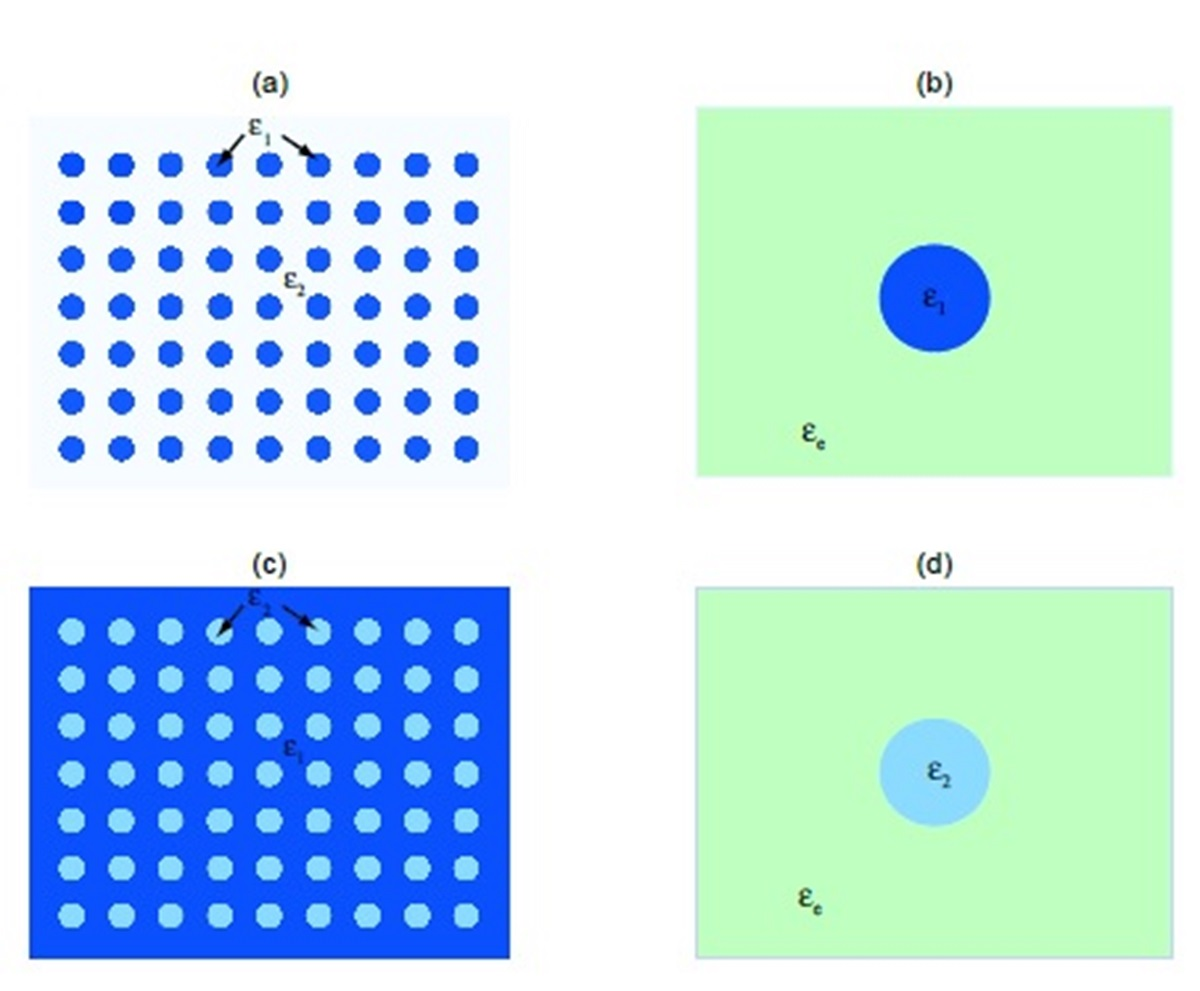
\includegraphics[width=9cm]{../Images/medio}
	\caption{\emph{Diagrama de (a) esferas de constante dieléctrica $\epsilon_1$ inmersas en un medio dieléctrico $\epsilon_2$, (b) esfera aislada de constante dieléctrica $\epsilon_1$ inmersa en un medio efectivo $\epsilon_e$, (c) esferas de constante dieléctrica $\epsilon_2$ inmersas en un medio dieléctrico $\epsilon_1$, (d) esfera aislada de constante diléctrica $\epsilon_2$ inmersa en un medio dieléctrico efectivo $\epsilon_e$}}
	\label{fig:ME}
\end{figure}

Supongamos también que el sistema de la Figura \ref{fig:MTT}(a) existe un campo eléctrico externo. \\
El punto de vista macroscópico, se se pone atención a una sóla esfera, se puede suponer que el campo eléctrico promedio afuera de la esfera corresponde al campo eléctrico promedio en todo el medio, es decir; se puede suponer que una esfere dieléctrica (con constante dieléctrica $\epsilon_1$) se encuentra inmersa en un medio dieléctrico efectivo (con constante dieléctrica $\epsilon_e$), como se muestra en la Figura \ref{fig:MTT} (b). Así, la constante dieléctrica $\epsilon_e$ será resultante de la mezcla de las costantes dieléctricas $\epsilon_1$ y $\epsilon_2$.\\
Consideramos el problema general de una esfere dieléctrica inmersa en un medio dieléctrico, sujeta a un campo eléctrico externo. Por lo tanto, el campo en el interior de la esfera estaría dado por:
\begin{equation}
E^{int}_1= \frac{3\epsilon_e}{2\epsilon_e + \epsilon_1} E^{ext}
\end{equation}
donde $E^{ext}$ es la magnitud del campo eléctrico externo. Por otro lado, si se considera el sistema opuesto donde las esferas están compuestas por el medio de constante dieléctrica $\epsilon_2$, inmersas en el medio de constante dieléctrica $\epsilon_1$ (ver la Figura \ref{fig:MTT} (c)), el campo eléctrico interior de la esfera la Figura \ref{fig:MTT} (d) estaría dado por
\begin{equation}
E^{int}_2=\frac{3\epsilon_e}{2\epsilon_e+\epsilon_2} E^{ext}
\end{equation}

Suponiendo que la fracción de cada uno de los medios, representadas por $f_1$ y $f_2$, sea la misma para ambos sistemas, entonces el campo macroscópico promedio de la mezcla se puede definir como la suma de los campos de cada uno de los componentes, siempre que el tamaño de las esferas sea mucho menor que el tamaño de todo el sistema y de la longitud de onda incidente.\\
Así, el campo interior de todas las esferas $\epsilon_1$ más el campo interior de todas las esferas $\epsilon_2$ será igual al campo total externo:

\begin{equation}
\begin{split}
E^{ext} &= f_1 \frac{3 \epsilon_e}{2\epsilon_e + \epsilon_1} E^{ext}+ f_2 \frac{3 \epsilon_e}{2\epsilon_e + \epsilon_2} E^{ext}\\
1 &= f_1 \frac{3\epsilon_e}{2\epsilon_e+\epsilon_1}+ f_2 \frac{3\epsilon_e}{2\epsilon_e+\epsilon_2}
\end{split}
\end{equation}


Haciendo un poco de álgebra, la expresión anterior se puede reescribir como
\begin{equation}
f_1 \frac{\epsilon_e - \epsilon_1}{\epsilon_1 + 2 \epsilon_e} + f_2 \frac{ \epsilon_2 - \epsilon_2 } {\epsilon_2+ 2\epsilon_e} =0 
\end{equation}



Esta expresión es llamada ecuación de Bruggeman para dos medios. Ésta relaciona la constante dieléctrica efectiva $\epsilon_e$ con las constantes dieléctricas de cada medio ($\epsilon_1$ y $\epsilon_2$).\\
Al aplicar la ecuación de Bruggeman al SP se tendría:

\begin{equation}\label{Eq:E1}
p \frac{\epsilon_{SP} - \epsilon_{Air}} {\epsilon_{Air}+2 \epsilon_{SP}} + (1-p) \frac {\epsilon_{SP} - \epsilon_{Si}} {\epsilon_{Si} +2\epsilon_{SP}} =0 ,
\end{equation}

donde $\epsilon_{SP}$, $\epsilon_{Si}$, $ \epsilon_{Air}$ corresponden a las constantes dieléctricas del SP (medio efectivo), silicio y aire, respectivamente, y p es la porosidad de la estructura. Al usa la relación n $\approx$ $\sqrt{\epsilon}$ (para medios dieléctricos) la Ecuación \textbf{\ref{Eq:E1}} se puede reescribir como

\begin{equation}\label{Eq:E2}
p \frac{n^{2}_{sp} - n^{2}_{Air}}{n^{2}_{Air} + 2 n^{2}_{Sp}} + (1-p) \frac{\epsilon_{SP} - \epsilon_{Si}}{\epsilon_{Si} +2\epsilon{Sp}}=0
\end{equation}


donde $n_{Sp}$, $n_{Si}$,  $n_{Air}$ corresponden a los índices de refracción del SP, silicio y aire, respectivamente. \\
Haciendo un poco de álgebra a la Ec. \textbf{\ref{Eq:E2}}, ésta se puede expresar como

\begin{equation}\label{Eq:E3}
n^{4}_{Sp} + \frac {(3P-2) n^{2}_{Si} - (3P-1) n^{2}_{Air}}{2} n^{2}_{Sp} - \frac{(n^{2}_{Si})(n^{2}_{Air})}{2}=0
\end{equation}

Al resolver la Ec \textbf{\ref{Eq:E3}} para $n_{Sp}$ se obtiene:

\begin{equation}\label{Eq:E4}
n_{Sp}= \pm \frac{1}{2} \sqrt{-T_1 \pm \sqrt{8(n^{2}_{Si})(n^{2}_{Air}) + (T_1)^{2}}}
\end{equation}

donde $T_1$=(3P-2) $n^2_{Si}$ - (3P-1) $n^{2}_{Air}$. La Ecuación \textbf{\ref{Eq:E4}} nos permite obtener una solución (que tenga sentido físico) para el índice de refracción correspondiente al SP, para una porosidad dada, un índice de refracción del silicio cristalino y el índice de refracción del aire.\\
Ahora, si considera al SP formado de cilindros de dieléctrico en lugar de esferas, al hacer un análisis similar al que se hizo anteriormente, se obtendría la ecuación de Bruggeman siguiente:


\begin{equation}\label{Eq:E5}
p\frac{n^{2}_{Sp}-n^{2}_{Air}}{n^{2}_{Air}+n^{2}_{Sp}}+(1-p) \frac{n^{2}_{Sp}-n^{2}_{Si}}{n^{2}_{Si}+n^{2}_{sp}}=0
\end{equation}

donde $n_{sp}$, $n_{si}$ , $n_{air}$ corresponden a los índices de refracción del SP (medio efectivo), silicio y aire, respectivamente. Similarmente, la Ec \textbf{\ref{Eq:E5}}, se puede expresar como:

\begin{equation} \label{Eq:E6}
n^{4}_{sp}+(2P-1)(n^{2}_{si}-n^{2}_{Ais}) n^{2}_{sp}- (n^{2}_{Si})(n^{2}_{Air})=0
\end{equation}

Al volver la Ec \textbf{\ref{Eq:E6}} para $n_{sp}$ se obtiene: 
{\small 
\begin{equation} \label{Eq:E7}
n_{sp} = \pm \frac{1}{\sqrt{2}} \sqrt{-(2P-1)(n^{2}_{Si} - n^{2}_{Air}) \pm \sqrt { 4(n^{2}_{Si})(n^{2}_{Air}) + (2P-1)^{2} (n^{2}_{Si} - n^{2}_{Air})^{2}}}
\end{equation} }

La Ec \textbf{\ref{Eq:E7}}  al igual que la Ec \textbf{\ref{Eq:E4}} nos permite obtener una solución (que tenga sentido físico) para el índice de refracción correspondiente al SP pero con la diferencia que el modelado del SP se hace por medio de cilindros en lugar de esferas.

\chapter{Microcavidades con Anodización Asimétrica}
\label{Mo:MiCROAA}
\markboth{CAPÍTULO 3. Microcavidades con Anodización Asimétrica}{}
\section{Resumen}
Describimos un estudio  experimental de las  microcavidades de silicio poroso (PSMC)  con Anodización Asimétrica (AA). Las PSMC con AA consistían en dos reflectores Bragg (BR) con un defecto entre ellos. Fue fabricado por grabado electroquímico de solución acuosa de ácido fluoridico (HF) y etanol. Las microcavidades (MC) fueron sometidas a un proceso de oxidación térmica  (DTOP). De esta forma, obtuvimos un silicio poroso oxidado (OPS) que induce un cambio de la respuesta a la región IR al Visible. Después de la formación electroquímica, la PSMC con AA se separa electroquimicamente con disolvente y se transfiere mecánicamente a cuarzo (MCL). La caracterización de las MC y MCL se realizó mediante espectroscopia SEM  y UV-Vis-NIR. Comparamos las muestras MC y MCL con diferentes temperaturas 
(21\grad C, 300\grad C, 600\grad C y 800\grad C) en diferentes puntos de medición, encontrando una relación de la temperatura con el FWHM. Estos resultados abren la posibilidad de crear estructuras fotónicas basadas en silicio dentro del rango IR-Visibles en la misma muestra con diferentes porosidades y profundidades. 
\section{Introducci\'on}
El comportamiento y la estructuras de los materiales nanoestructurados se ha convertido en un gran tema de interés mundial donde ha resultado numerosas  investigación desde hace algún tiempo. Encontramos un gran camino por recorrer  para las futuras exploraciones tecnológicas, un sinnúmero de retos y desafíos que abre un abanico de posibilidades para desarrollar estudio mas avanzando sobre dichos temas \cite{I1}. El silicio poroso (PS) es un material nanoestructurado versátil y un excelente candidato como plataforma tecnológica para diferentes aplicaciones de sensado\cite{I2}. Esto último, gracias a su fácil fabricación, su grande área superficial, su alta reactividad de superficie, y sobre todo, por su capacidad de transducción óptica.
Una configuración de anodización asimétrica se obtienen muestras con un gradiente lateral en términos de tamaño de poro y espesor de la capa porosa. En esta configuración, la cara del electrodo de platino (cátodo) se mantiene relativamente perpendicular a la superficie del sustrato de Si (ánodo) en uno de los extremos de la celda, de tal forma que la distribución de la corriente dentro de la solución electrolítica varía en función de la distancia del electrodo debido a la resistencia del electrolito, resultando en una disminución de la densidad de corriente conforme la distancia desde el electrodo aumenta. El resultado es una superficie porosa con diferentes tamaños de poros que van desde unos cuantos nanómetros hasta poros del orden de unos cuantos micrómetros. Las dimensiones de los poros obtenidos en el mismo chip pueden controlarse ajustando la corriente de anodización y la concentración del electrólito \cite{I3}. Actualmente, este tipo de muestras han encontrado relevante su aplicación como filtros de banda ópticos\cite{I3}, dispositivos con banda fotónicas multidireccional (códigos de barra fotónicos)\cite{I4} y principalmente, como biosensores. De esta forma, se estudia el efecto que ejercen diferentes topografías (porosidades en la misma muestra) en el cultivo/adhesión de ciertas células \cite{I5 ,I6}, reduciendo considerablemente la cantidad de muestras y costo del estudio. Además, también son muy útiles cuando se requiere una técnica de exclusión por tamaño de biomoléculas permitiendo la identificación y separación de estos compuestos biológicos \cite{I7}.\\ 
Este trabajo esta organizado de la siguiente manera. En la Sección 2, los detalles experimentales de como se  fabricaron las  microcavidades (MC) silicio poroso (PS) con anodización asimétrica (AA)    mediante un grabado electroquímico en una oblea de silicio a través de una configuración de electrodo asimétrica en solución acuosa de HF etanólico. En la sección 3, hacemos la discusión de los resultado comparando los resultados obtenidos y en la Sección 4, las conclusiones. 
\section{Detalles Experimentales}
\begin{figure}[H]
	\centering
	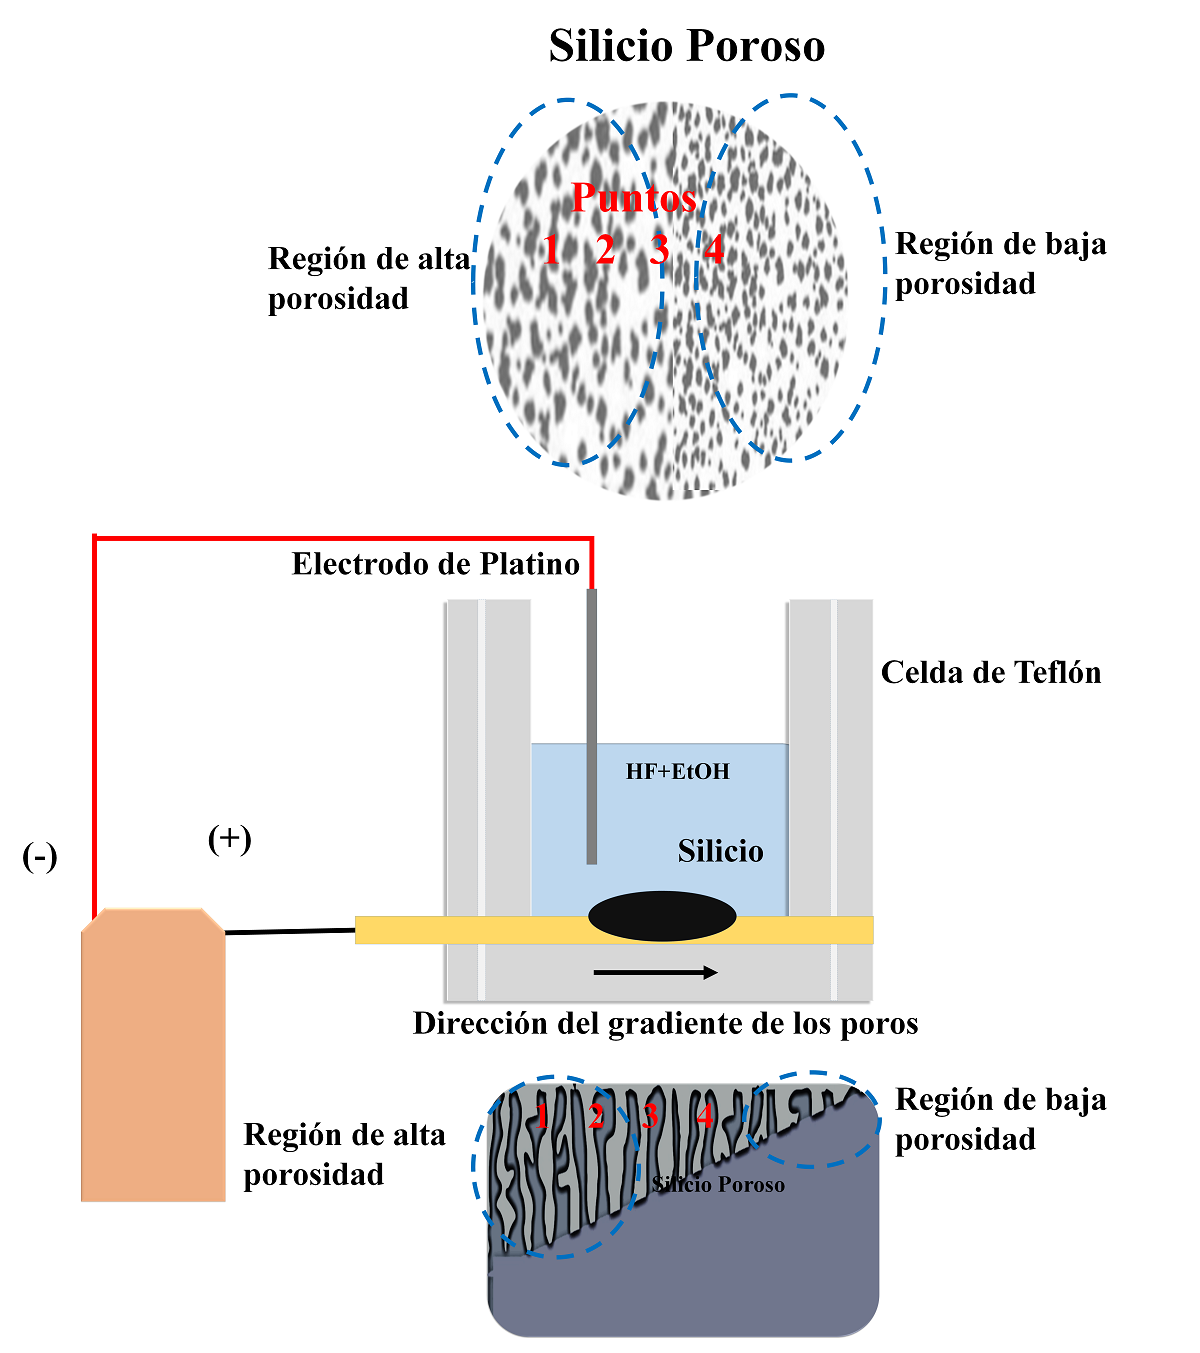
\includegraphics[scale=.3]{../Images/EPS0}
	\caption{\emph{Esquema de la celda electroquímica  para una configuración con anodización asimétrica. Se muestra  un gradiente lateral en términos de tamaño de poro y espesor de la capa porosa. En esta configuración, la cara del electrodo de platino (cátodo) se mantiene relativamente perpendicular a la superficie del sustrato de Si (ánodo) en uno de los extremos de la celda  }}
	\label{fig:p0}
\end{figure}
Algunas de las estructuras fotónicas simuladas se fabricaron mediante grabado anódico de una oblea de Si cristalina de tipo p orientada (100) (resistividad 0.002 - 0.005 $ \Omega \cdot cm$), en condiciones galvanostáticas. Las muestras se prepararon de forma similar a la descrita anteriormente en Y.L Khung et al. \cite{Ik}. El proceso de anodización electroquímica se realizó a temperatura ambiente, con una mezcla electrolítica de ácido fluorhídrico (HF) (concentración: 48 $ \% $ de peso), glícerol (pureza: 99.8$ \% $ de peso) y etanol (pureza: 99.9$ \% $ de peso) en 3: 7 : 1 proporción de volumen, respectivamente. Colocando la oblea del silicio a la superficie de la celda electrolitica y el electrodo de platino perpendicular en un extremo como se ve en la Figura \ref{fig:p0}. Después del proceso de anodización, las muestras se enjuagan con etanol (pureza: 99,9$ \% $ en peso). Las microcavidades (MC) de silicio poroso con Anodización Asimétrica (AA), fueron fabricadas con diferentes  corrientes $(I_1I_2)_5I_1I_2(I_1I_2)_5$, la primera de $I_1=4.8 \ \  mA$ y la otra de  $I_2=38.7 \ \  mA$, con tiempos de ataque $t_1=39s$ y $t_2=9s$, sobre un área de $1.2 \ \ cm^2$. El cátodo esta constituido de un alambre de platino que fue arreglado en forma de una punta de diámetro aproximado de ($0.5\ \ mm$). Después de la formación electroquímica, la PSMC con AA se separa electroquimicamente con disolvente y se transfiere mecánicamente a cuarzo (MCL), siguiendo el procedimiento de \cite{I10L}. Las mediciones de reflectividad se llevaron a cabo con un espectrofotómetro UV-Vis-NIR Perkin Elmer Lambda 950. Las morfologías de las capas porosas grabadas ( transversal) se observaron utilizando microscopios electrónicos de barrido SEM Hitachi SU1510 (Hitachi High Technologies Canada, Inc., Toronto, Canadá).
El tratamiento térmico(  300\grad C ,  600\grad C ,  800\grad C) para las Microcavidades de silicio poroso con Anodización Asimétrica para MC y MCL,  fueron  a través de resistencias eléctricas y horno usado para oxidar las muestras(Horno tubular (GSL-1500X) ).  

\section{Discusión y Resultados}
\subsection{Microcavidades de silicio poroso con Anodización Asimétrica}
\begin{figure}[H]
	\centering
	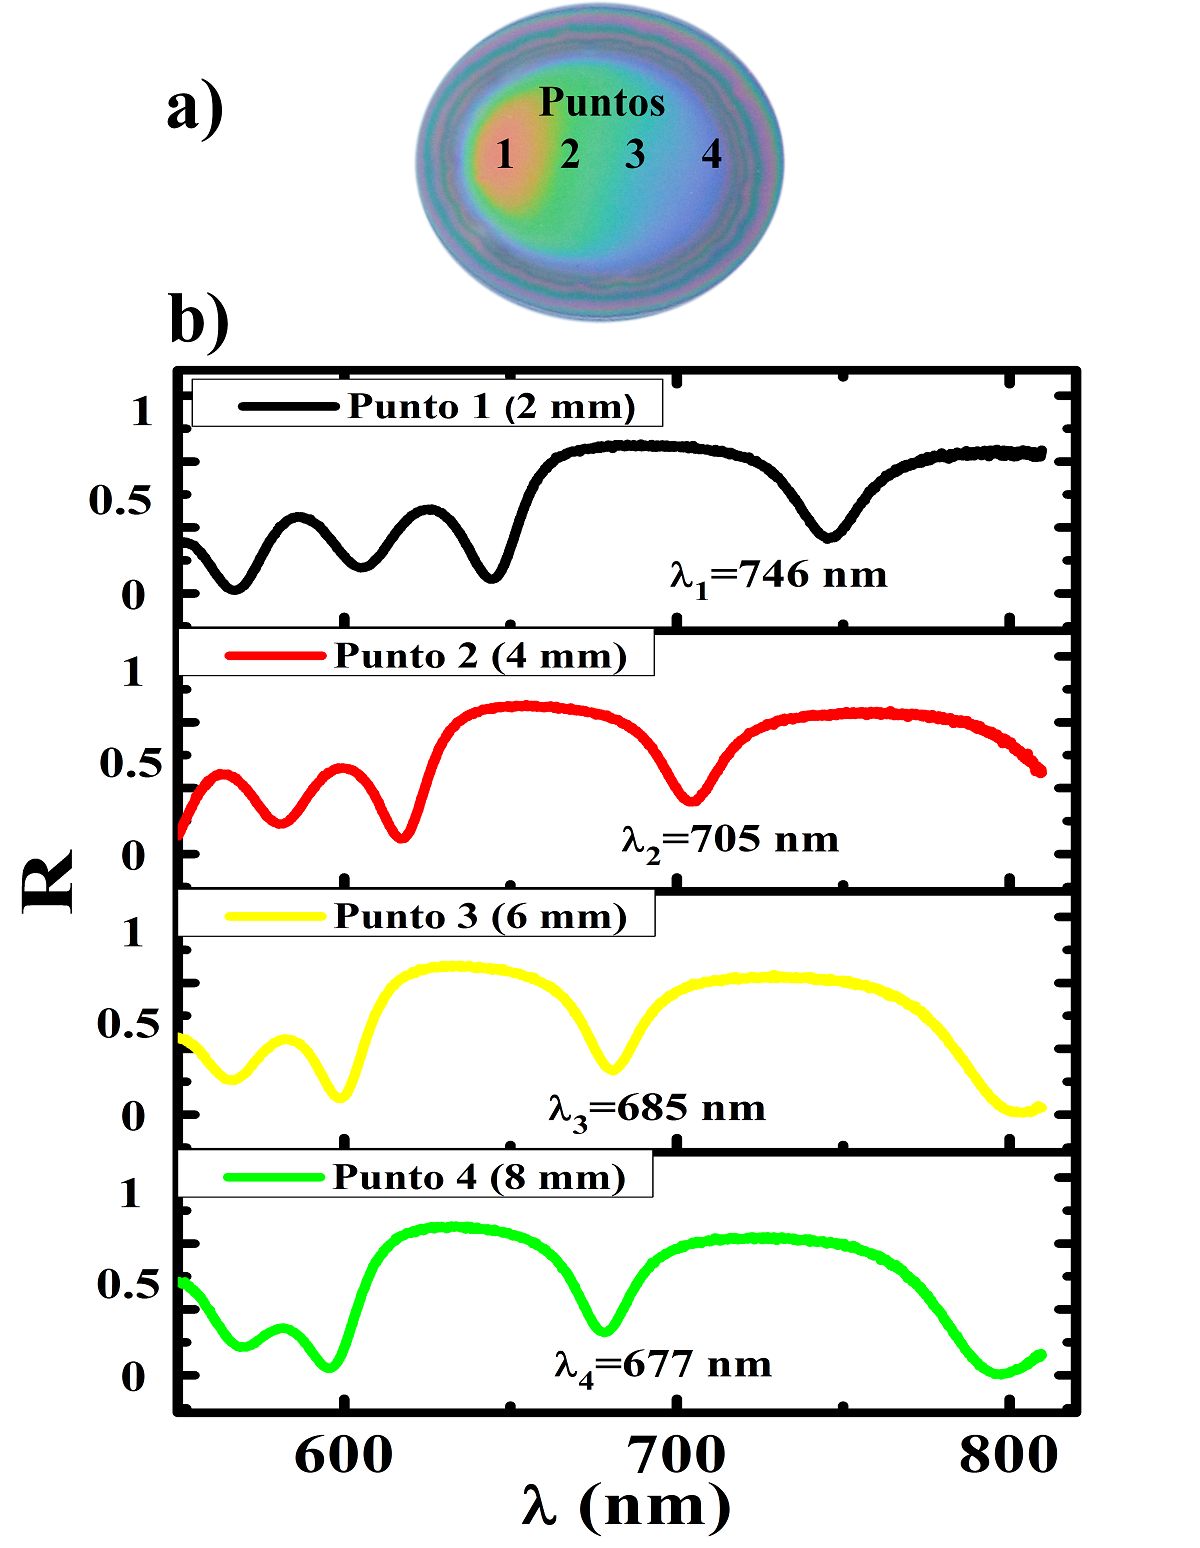
\includegraphics[scale=.25]{../Images/PsiR1}
	\caption{\emph{Muestra de la Microcavidad (MC) de silicio poroso con Anodización Asimétrica que fue fabricada con diferentes  corrientes $(I_1I_2)_5I_1I_2(I_1I_2)_5$, la primera de $I_1=4.8 \ \  mA$ y la otra de  $I_2=38.7 \ \  mA$, con tiempos de ataque de $t_1=39s$ y $t_2=9s$ , sobre un área de $1.2 \ \ cm^2$. a) La muestra $MC_{_{21^{\circ} C}}$, tenemos los puntos de medición indicados (1(2mm),2(4mm),3(6mm) y 4(8mm)), donde el punto 1 esta  cerca del el electrodo y el punto 4 mas alejado del electrodo, como se  observa en la Figura \ref{fig:p0}. b) Los espectros de reflectancia  en función de la longitud de onda (nm) medidos en el punto 1 ($\lambda_{_{1}}=746 nm$), punto 2 ($\lambda_{_{2}}=705 nm$), punto 3 ($\lambda_{_{3}}=685 nm$) y punto 4 ($\lambda_{_{4}}=677 nm$). }}
	\label{fig:p1}
\end{figure}

La Figura \textbf{\ref{fig:p1}} se muestra la microcavidad (MC) de silicio poroso con anodización asimétrica (AA), que fue fabricada con diferentes  corrientes $(I_1I_2)_5I_1I_2(I_1I_2)_5$, la primera de $I_1=4.8 \ \  mA$ y la otra de  $I_2=38.7 \ \  mA$, con tiempos de ataque de $t_1=39s$ y $t_2=9s$ , sobre un área de $1.2 \ \ cm^2$. La Figura \textbf{\ref{fig:p1} a)} La muestra $MC_{_{21^{\circ} C}}$, tenemos los puntos de medición (1(2mm),2(4mm),3(6mm) y 4(8mm)), donde el punto 1 esta  cerca del el electrodo y el punto 4 mas alejado del electrodo, como se  observa en la Figura \textbf{\ref{fig:p0}} de la sección 2. En la Figura \textbf{\ref{fig:p1} b)}  mostramos los espectros de reflectancia($\%$) en función de la longitud de onda (nm)  medidos en el punto 1 ($\lambda_{_{1}}=746 nm$), punto 2 ($\lambda_{_{2}}=705 nm$), punto 3 ($\lambda_{_{3}}=685 nm$) y punto 4 ($\lambda_{_{4}}=677 nm$). Y medidos los anchos medios de los picos FWHM (Full Width at Half Maximum) en cada punto de medición  22.1 nm (Para en punto 1),  23.2 nm (Para en punto 2),  19.4 nm (Para en punto 3) y  19.8 nm (Para en punto 4). 
\begin{figure}[H]
	\centering
	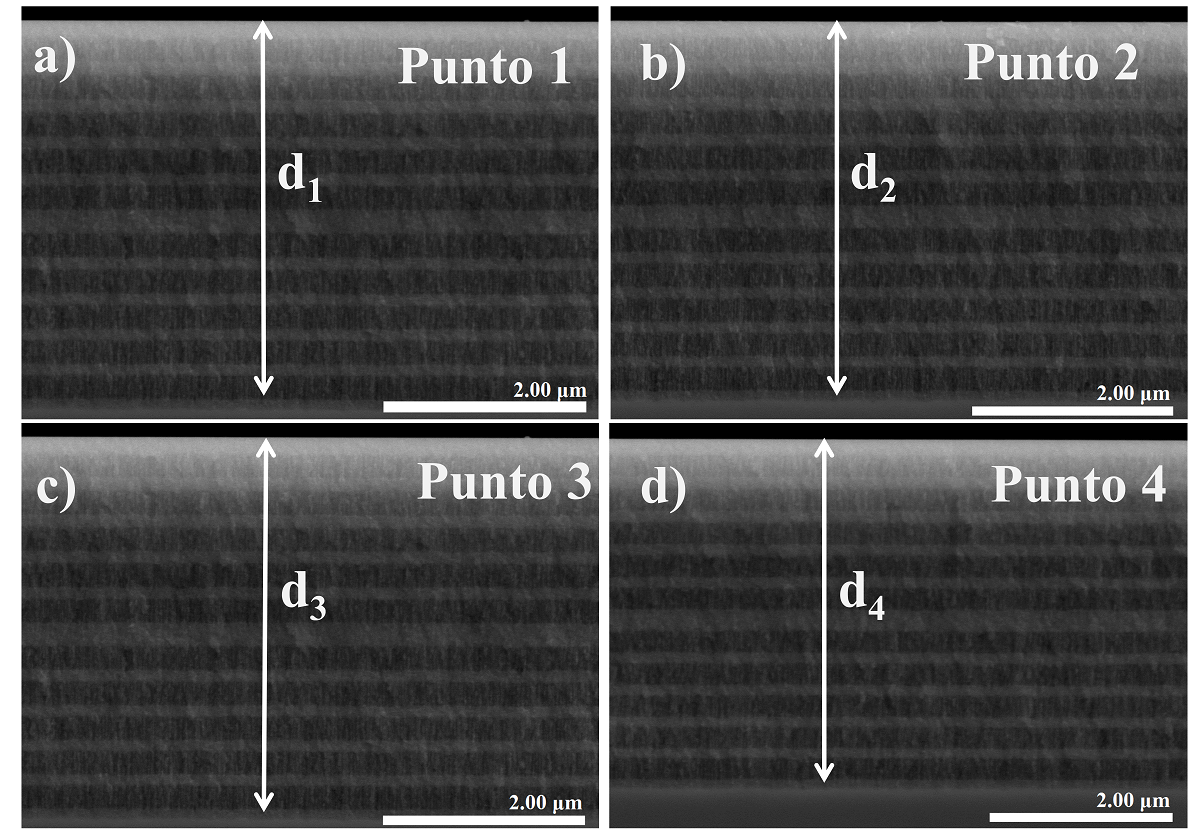
\includegraphics[scale=.3]{../Images/Sem1}
	\caption{\emph{Micrografias de la sección trasversal de SEM de  microcavidades de silicio poroso con anodización asimétrica, donde podemos medir la profundidad $d_{_{i}}$ (i=1,2,3,4) de la estructura. Para cada muestra tenemos los puntos de medición calculando  el espesor físico total : a) el punto 1 ($d_{_{1}}=3.8 \mu m$), b) punto 2 ($d_{_{2}}=3.6 \mu m$), c) punto 3 ($d_{_{3}}= 3.4 \mu m$) y d) punto 4 ($d_{_{4}}=3.1 \mu m$).}}
	\label{fig:p2}
\end{figure}
La Figura \textbf{\ref{fig:p2}} mostramos las micrografias de la sección Trasversal de SEM de  Microcavidades de silicio poroso con Anodización Asimétrica, donde podemos medir la profundidad de la estructura. Para cada muestra tenemos los puntos de medición calculando  el espesor físico total $d_{_{i}}$ (i=1,2,3,4), las Figuras \textbf{\ref{fig:p2}} nos muestran,   a) el punto 1 ($d_{_{1}}=3.8 \mu m$), b) punto 2 ($d_{_{2}}=3.6 \mu m$), c) punto 3 ($d_{_{3}}= 3.4 \mu m$) y d) punto 4 ($d_{_{4}}=3.1 \mu m$) respectivamente. Pudiendo ver  el tamaño de la estructura total, viendo las disminución en cada punto de medición.

\subsection{Tratamiento térmico de Microcavidades}
\begin{figure}[H]
	\centering
	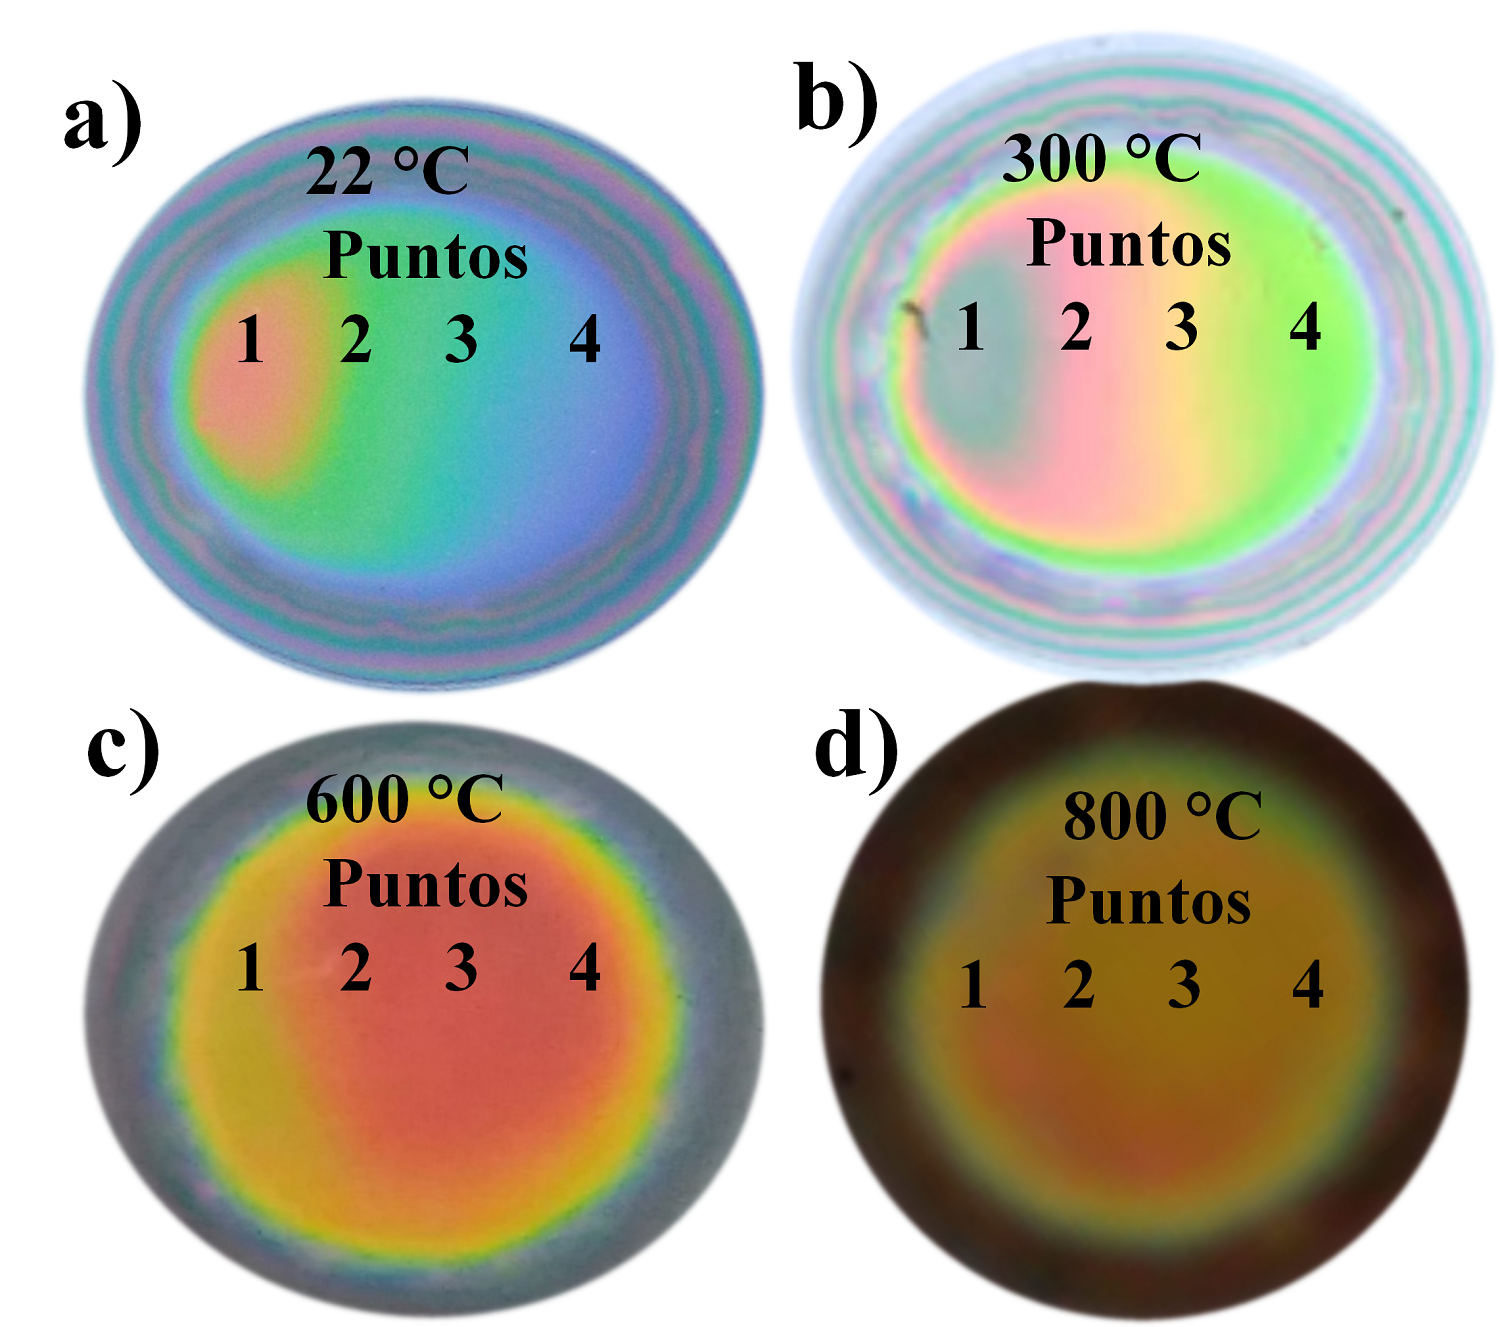
\includegraphics[scale=.15]{../Images/PsiTem}
	\caption{\emph{Fotografías de las  microcavidades de silicio poroso con anodización asimétrica. Para cada muestra tenemos los puntos de medición indicado (1(2mm),2(4mm),3(6mm) y 4(8mm)), donde el punto 1 esta por cerca del el electrodo y el punto 4 mas alejado del electrodo.  La temperatura ($^{\circ}C$) utilizada para el tratamiento térmico ( 300\grad C ,  600\grad C ,  800\grad C) en cada una de las  muestras a) $MC_{_{21^{\circ} C}}$, b) $MC_{_{300^{\circ} C}}$, c) $MC_{_{600^{\circ} C}}$ y d) $MC_{_{800^{\circ} C}}$.}}
	\label{fig:p3}
\end{figure}
En la Figura \textbf{\ref{fig:p3}} son las fotografías de las   Microcavidades de silicio poroso con Anodización Asimétrica. Para cada muestra tenemos los puntos de medición indicado (1(2mm),2(4mm),3(6mm) y 4(8mm)), donde el punto 1 esta por cerca del el electrodo y el punto 4 mas alejado del electrodo.  La temperatura ($^{\circ} C$) utilizada para el tratamiento térmico (300\grad C ,  600\grad C ,  800\grad C) en cada una de las  muestras, las Figuras \textbf{\ref{fig:p3}} a), b), c), d) nos muestran, $MC_{_{21^{\circ} C}}$,  $MC_{_{300^{\circ} C}}$,  $MC_{_{600^{\circ} C}}$ y $MC_{_{800^{\circ} C}}$, respectivamente. El tratamiento térmico   fueron  a través de resistencias eléctricas y horno usado para oxidar las muestras(Horno tubular (GSL-1500X)).
\begin{figure}[H]
	\centering
	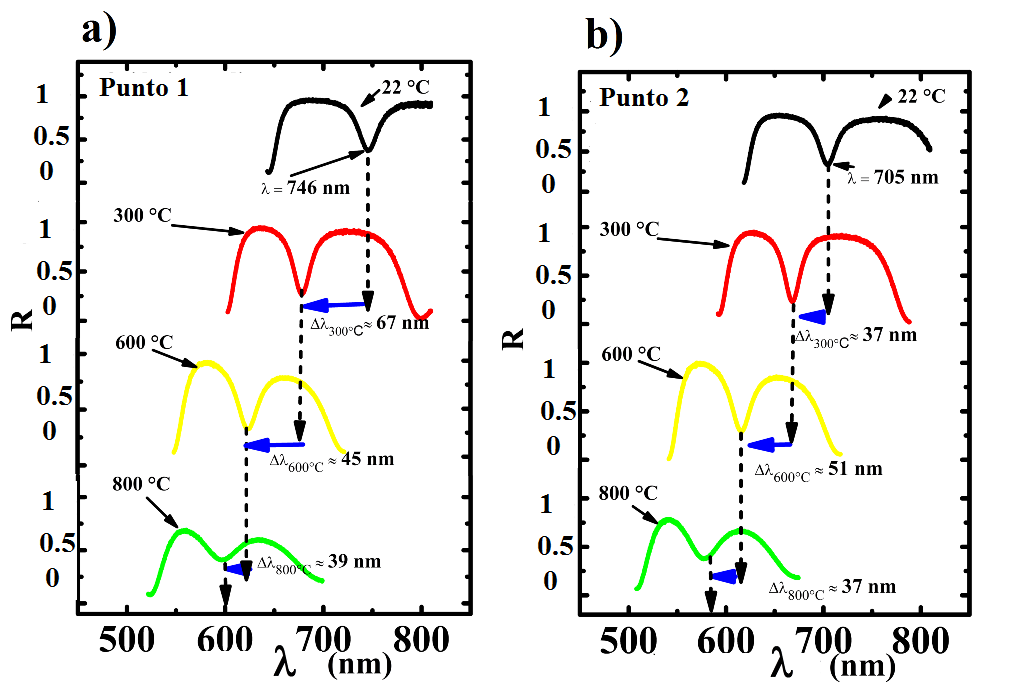
\includegraphics[scale=.35]{../Images/p2}
	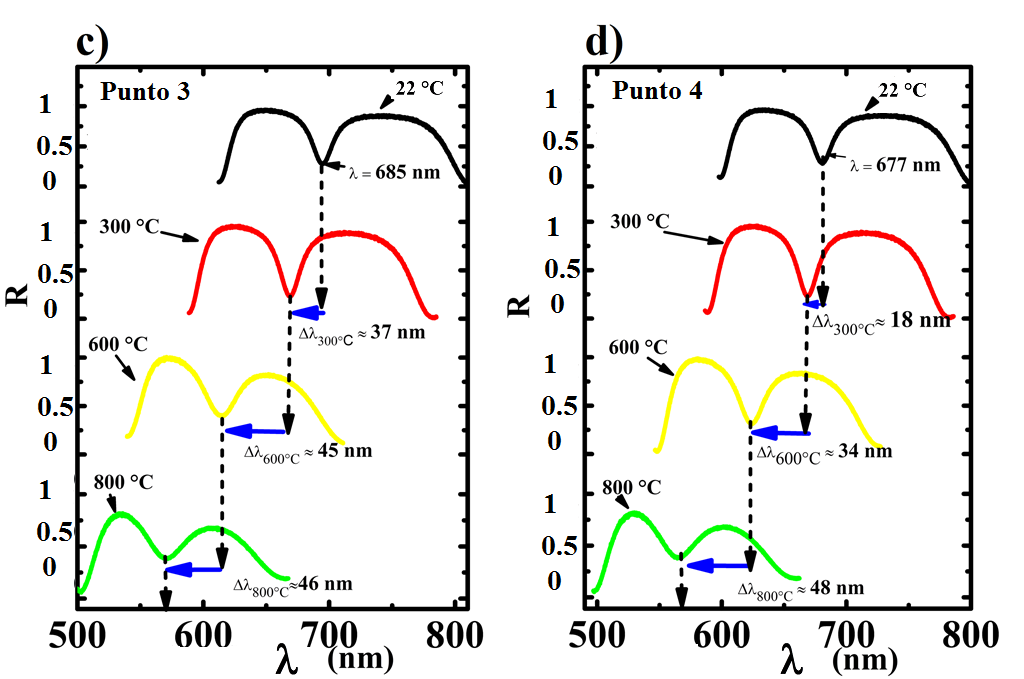
\includegraphics[scale=.35]{../Images/p3}
	\caption{\emph{Espectro de reflectancias ($\%$) en función de la longitud de onda (nm), de las microcavidades de silicio poroso con Anodización Asimétrica (MC) y se le dio tratamiento térmico, como se indica en la Figura \ref{fig:p3}. a) Comparamos la diferencias de picos en el punto 1, $\Delta \lambda_{_{300^{\circ} C}}=67 nm$,  $\Delta \lambda_{_{600^{\circ} C}}=45 nm$ y  $\Delta \lambda_{_{800^{\circ} C}}=39 nm$. b) Comparamos la diferencias de picos en el punto 2, $\Delta \lambda_{_{300^{\circ} C}}=37 nm$,  $\Delta \lambda_{_{600^{\circ} C}}=51 nm$ y  $\Delta \lambda_{_{800^{\circ} C}}=37 nm$. c) Lo mismo para este punto 3, $\Delta \lambda_{_{300^{\circ} C}}=37 nm$,  $\Delta \lambda_{_{600^{\circ} C}}=45 nm$ y  $\Delta \lambda_{_{800^{\circ} C}}=46 nm$. d) Y para el punto 4,  $\Delta \lambda_{_{300^{\circ} C}}=18 nm$,  $\Delta \lambda_{_{600^{\circ} C}}=34 nm$ y  $\Delta \lambda_{_{800^{\circ} C}}=48 nm$ }}
	\label{fig:p4}
\end{figure}
En la Figura \textbf{\ref{fig:p4} a)}  mostramos los espectros de reflectancia($\%$) en función de la longitud de onda (nm), para el punto 1 de las diferentes muestras, con sus diferentes tratamiento térmico para $21^{\circ} C$ ($\lambda_{_{1}}=746 nm$) ,  $300^{\circ} C$ ($\lambda_{_{1}}=679 nm$), $600^{\circ} C$ ($\lambda_{_{1}}=624 nm$) y  $800^{\circ} C$ ($\lambda_{_{1}}=598 nm$), teniendo en cuenta las diferencias entre picos, $\Delta \lambda_{_{300^{\circ} C}}=67 nm$,  $\Delta \lambda_{_{600^{\circ} C}}=45 nm$ y  $\Delta \lambda_{_{800^{\circ} C}}=39 nm$. De la Figura \textbf{\ref{fig:p4} a)} sacamos  los anchos medios de los picos FWHM (Full Width at Half Maximum)\cite{FMHW1, FMHW2, FMHW3} en cada punto de medición  22.1 nm (Para $21^{\circ} C$ en punto 1),  19.2 nm (Para $300^{\circ} C$ en punto 1),  20.5 nm (Para $300^{\circ} C$ en punto 1) y  28.4 nm (Para $300^{\circ} C$ en punto 1). Así mismo, en la Figura \textbf{\ref{fig:p4} b)}  para el punto 2 de las diferentes muestras, con sus diferentes tratamiento térmico para $21^{\circ} C$ ($\lambda_{_{2}}=705 nm$) ,  $300^{\circ} C$ ($\lambda_{_{2}}=667 nm$), $600^{\circ} C$ ($\lambda_{_{2}}=616 nm$) y  $800^{\circ} C$ ($\lambda_{_{3}}=579 nm$), teniendo en cuenta las diferencias entre picos, $\Delta \lambda_{_{300^{\circ} C}}=37 nm$,  $\Delta \lambda_{_{600^{\circ} C}}=51 nm$ y  $\Delta \lambda_{_{800^{\circ} C}}=37 nm$. De esa misma figura sacamos los FWHM, 23.2 nm (Para $21^{\circ} C$ en punto 2),  16.5 nm (Para $300^{\circ} C$ en punto 2),  19.5 nm (Para $300^{\circ} C$ en punto 2) y  26.3 nm (Para $300^{\circ} C$ en punto 2). Seguimos analizando la Figura \textbf{\ref{fig:p4} c)}  para el punto 3 de las diferentes muestras, con sus diferentes tratamiento térmico para $21^{\circ} C$ ($\lambda_{_{3}}=685 nm$) ,  $300^{\circ} C$ ($\lambda_{_{3}}=658 nm$), $600^{\circ} C$ ($\lambda_{_{3}}=613 nm$) y  $800^{\circ} C$ ($\lambda_{_{3}}=567 nm$), teniendo en cuenta las diferencias entre picos, $\Delta \lambda_{_{300^{\circ} C}}=37 nm$,  $\Delta \lambda_{_{600^{\circ} C}}=45 nm$ y  $\Delta \lambda_{_{800^{\circ} C}}=46 nm$ y  sacamos los FWHM, 23.2 nm (Para $21^{\circ} C$ en punto 3),  16.5 nm (Para $300^{\circ} C$ en punto 3),  19.5 nm (Para $300^{\circ} C$ en punto 3) y  26.3 nm (Para $300^{\circ} C$ en punto 3). Y por ultimo, de la Figura \textbf{\ref{fig:p4} d)} para el punto 4, con sus diferentes tratamiento térmico para $21 ^{\circ} C$ ($\lambda_{_{4}}=677 nm$) ,  $300^{\circ} C$ ($\lambda_{_{4}}=642 nm$), $600^{\circ} C$ ($\lambda_{_{4}}=608 nm$) y  $800^{\circ} C$ ($\lambda_{_{4}}=560 nm$), teniendo en cuenta las diferencias entre picos, $\Delta \lambda_{_{300^{\circ} C}}=18 nm$,  $\Delta \lambda_{_{600^{\circ} C}}=34 nm$ y  $\Delta \lambda_{_{800^{\circ} C}}=48 nm$ y  sacamos los FWHM, 19.8 nm (Para $21^{\circ} C$ en punto 4),  17.8 nm (Para $300^{\circ} C$ en punto 4),  21.7 nm (Para $300^{\circ} C$ en punto 4) y  25.2 nm (Para $300^{\circ} C$ en punto 4).

\subsection{Separación Electroquímica de Microcavidades }
\begin{figure}[H]
	\centering
	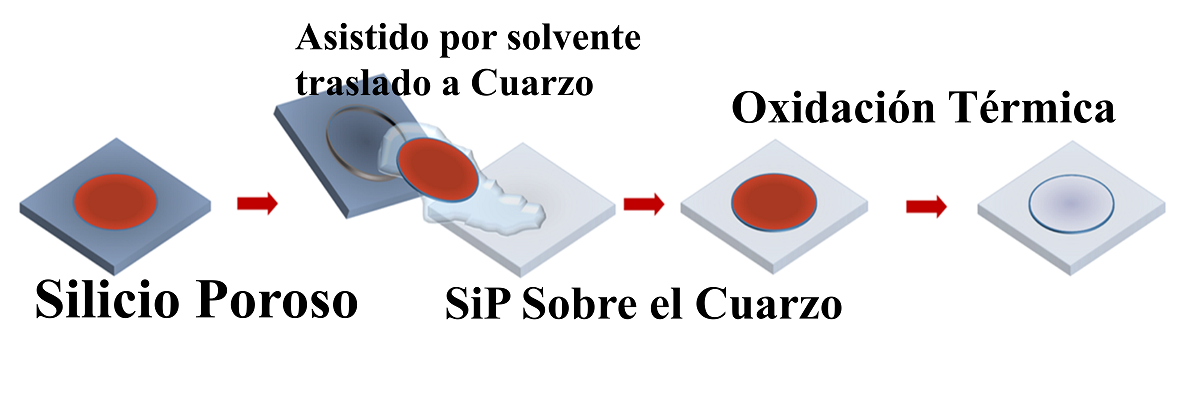
\includegraphics[scale=.35]{../Images/Spleva1}
	\caption{\emph{Esquema de  las microcavidades de silicio poroso con anodización asimétrica,  que se separa electroquimicamente con disolvente, luego se transfiere mecánicamente a cuarzo (MCL) y al final se le hace tratamiento térmico; siguiendo el procedimiento de }\cite{I10L}.}
	\label{fig:p6}
\end{figure}
En la Figura \ref{fig:p6}, se muestra el esquema de  las microcavidades de silicio poroso con anodización asimétrica,  que se separa electroquimicamente con disolvente, luego se transfiere mecánicamente a cuarzo (MCL) y al final se le hace tratamiento térmico. 
\begin{figure}[H]
	\centering
	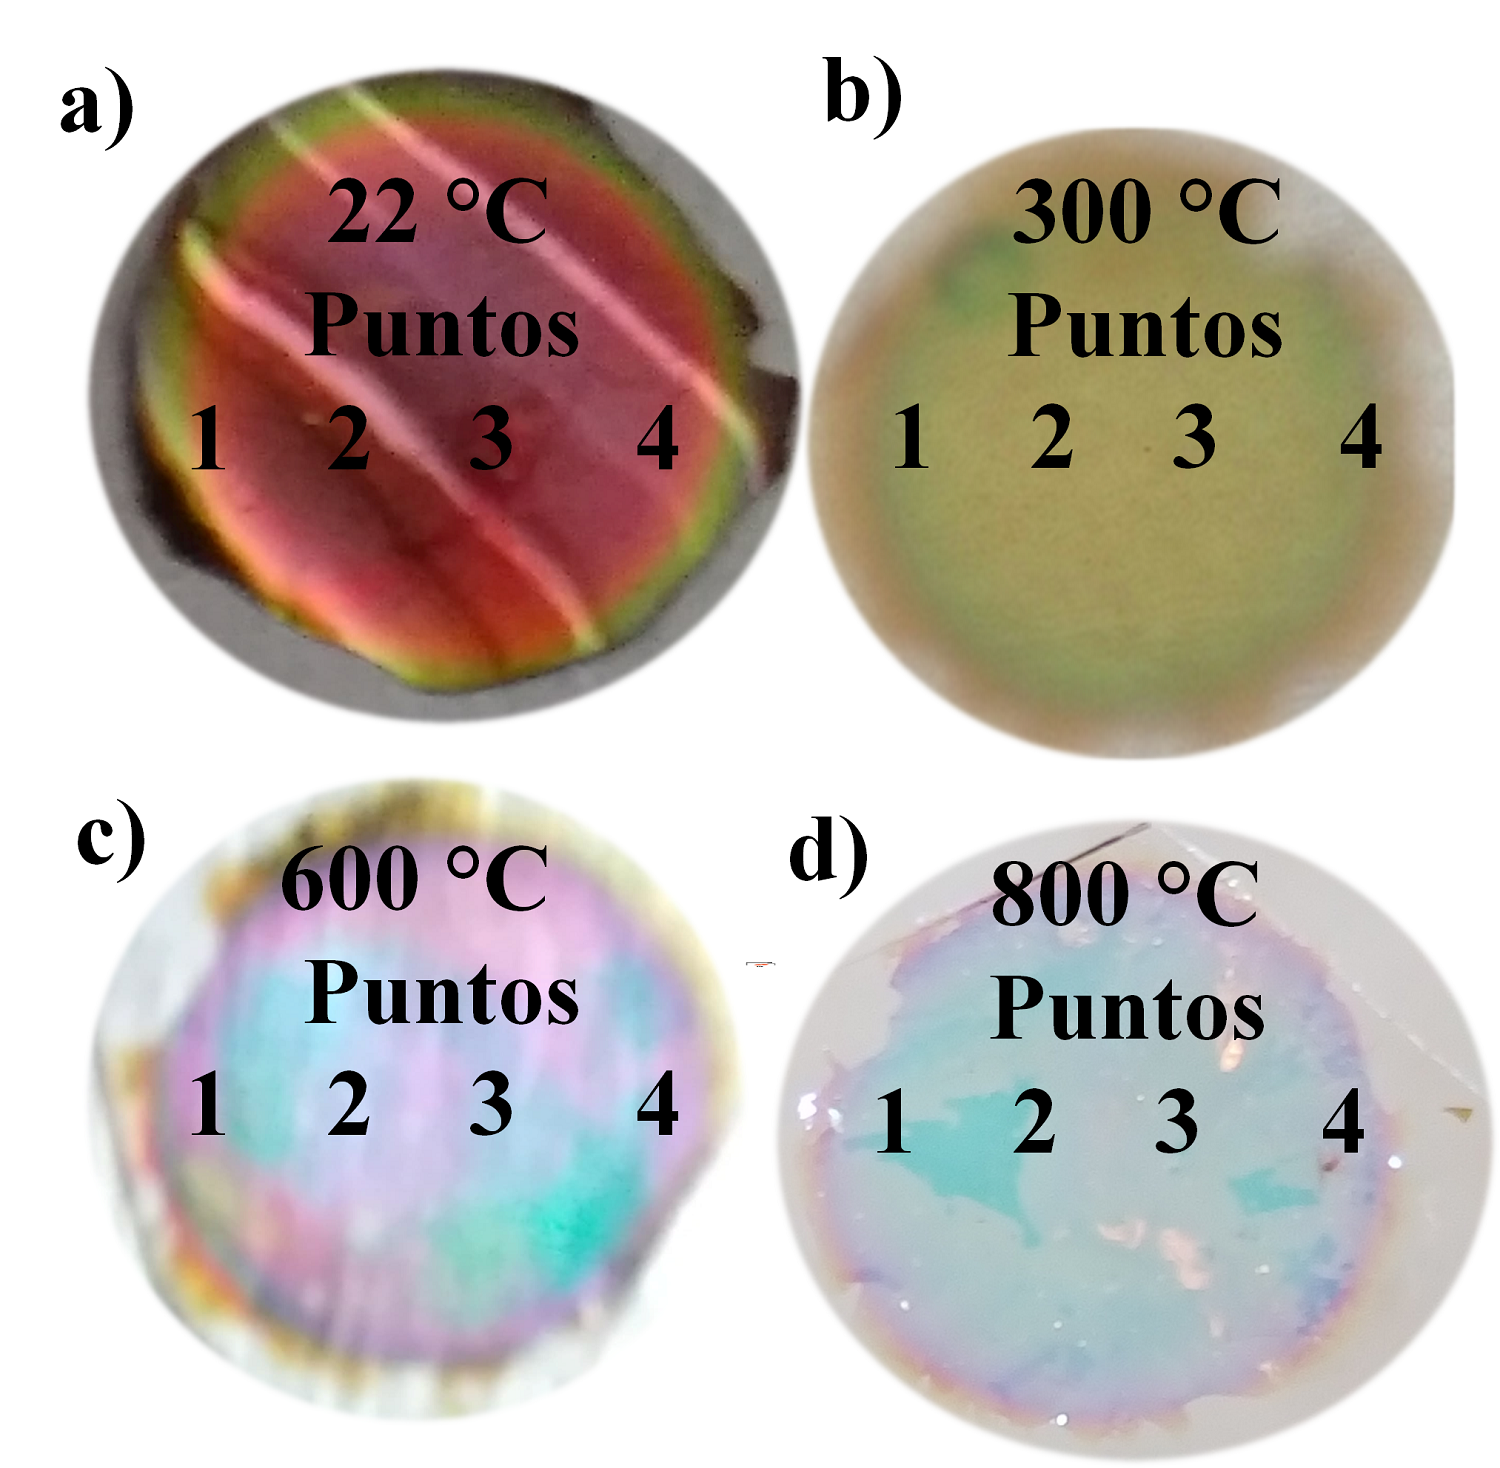
\includegraphics[scale=.15]{../Images/PsiTLa}
	\caption{\emph{Fotografías de las microcavidades de silicio poroso con Anodización Asimétrica que se separaron electroquimicamente con disolvente,  se transfiere mecánicamente a cuarzo (MCL) y al final se le dio tratamiento térmico. Para cada muestra tenemos los puntos de medición indicado (1(2mm),2(4mm),3(6mm) y 4(8mm)), donde el punto 1 esta por cerca del el electrodo y el punto 4 mas alejado del electrodo.  La temperatura ($^{\circ} C$) utilizada para el tratamiento térmico (300\grad C ,  600\grad C ,  800\grad C) en   las  muestras $MCL_{_{21^{\circ} C}}$, $MCL_{_{300^{\circ} C}}$, $MCL_{_{600^{\circ} C}}$ y $MCL_{_{800^{\circ} C}}$.}}
	\label{fig:p7}
\end{figure}
En la Figura \ref{fig:p3} son las fotografías de las microcavidades de silicio poroso con Anodización Asimétrica que se separaron electroquimicamente con disolvente,  se transfiere mecánicamente a cuarzo (MCL) y al final se le dio tratamiento térmico. Para cada muestra tenemos los puntos de medición indicado (1(2mm),2(4mm),3(6mm) y 4(8mm)), donde el punto 1 esta por cerca del el electrodo y el punto 4 mas alejado del electrodo.  La temperatura ($^{\circ} C$) utilizada para el tratamiento térmico (300\grad C ,  600\grad C ,  800\grad C) en cada muestra, las Figuras \textbf{\ref{fig:p2}} a), b), c), d) nos muestran, $MCL_{_{21^{\circ} C}}$,  $MCL_{_{300^{\circ} C}}$,  $MCL_{_{600^{\circ} C}}$ y $MCL_{_{800^{\circ} C}}$, respectivamente. El tratamiento térmico   fueron  a través de resistencias eléctricas y horno usado para oxidar las muestras(Horno tubular (GSL-1500X)).
\begin{figure}[H]
	\centering
	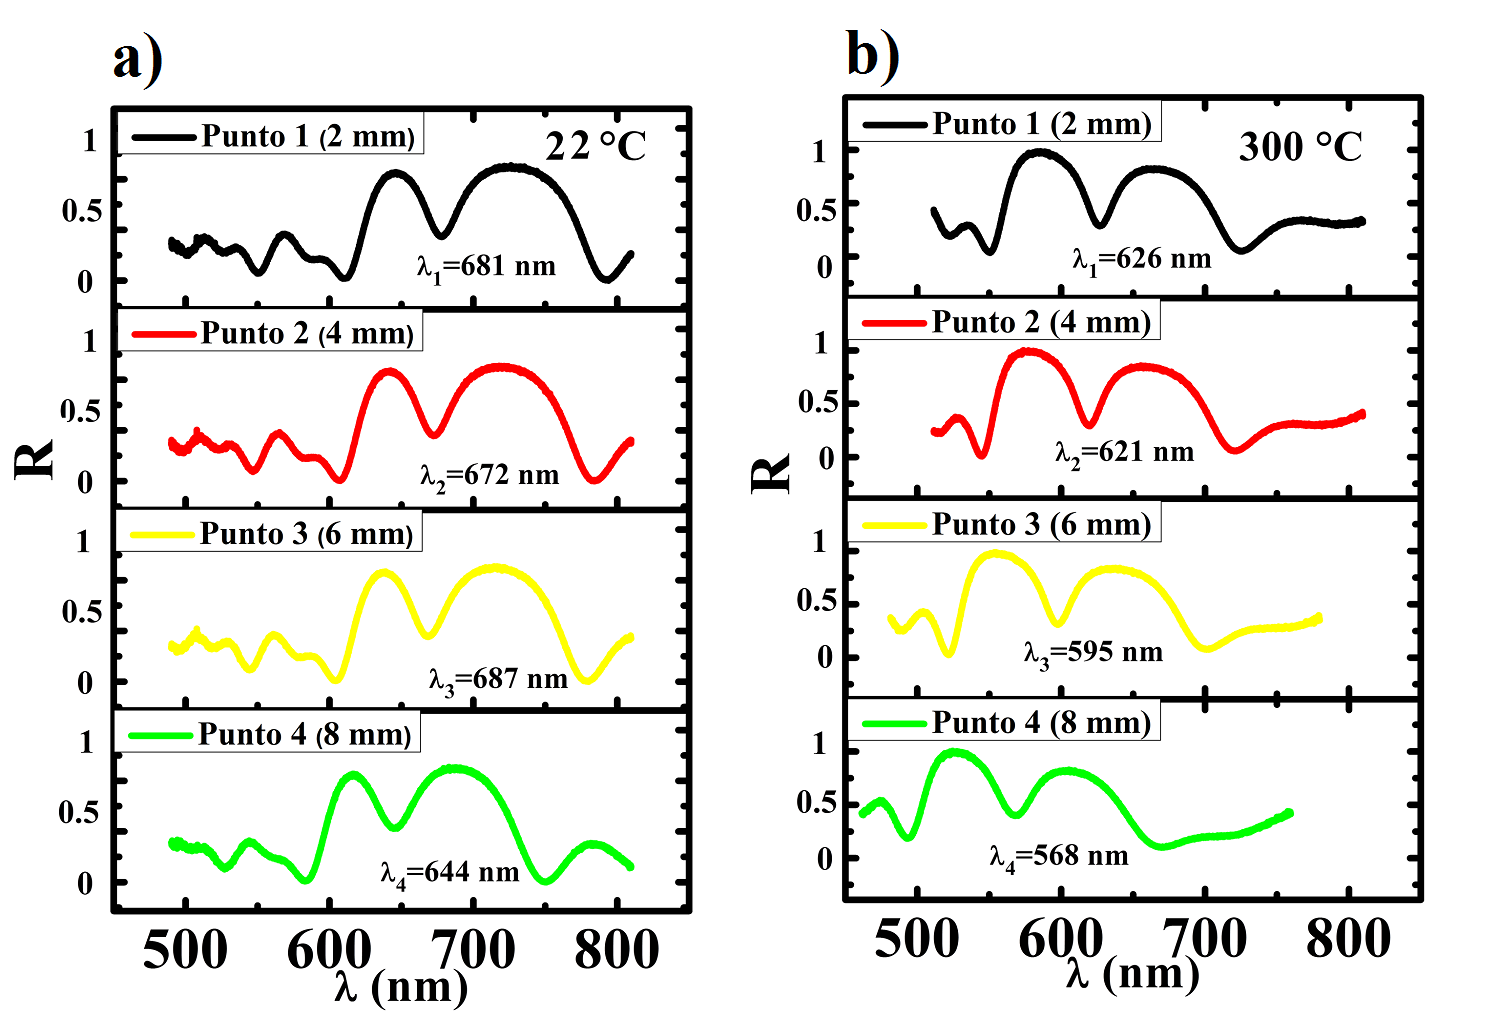
\includegraphics[scale=.25]{../Images/pl1}
	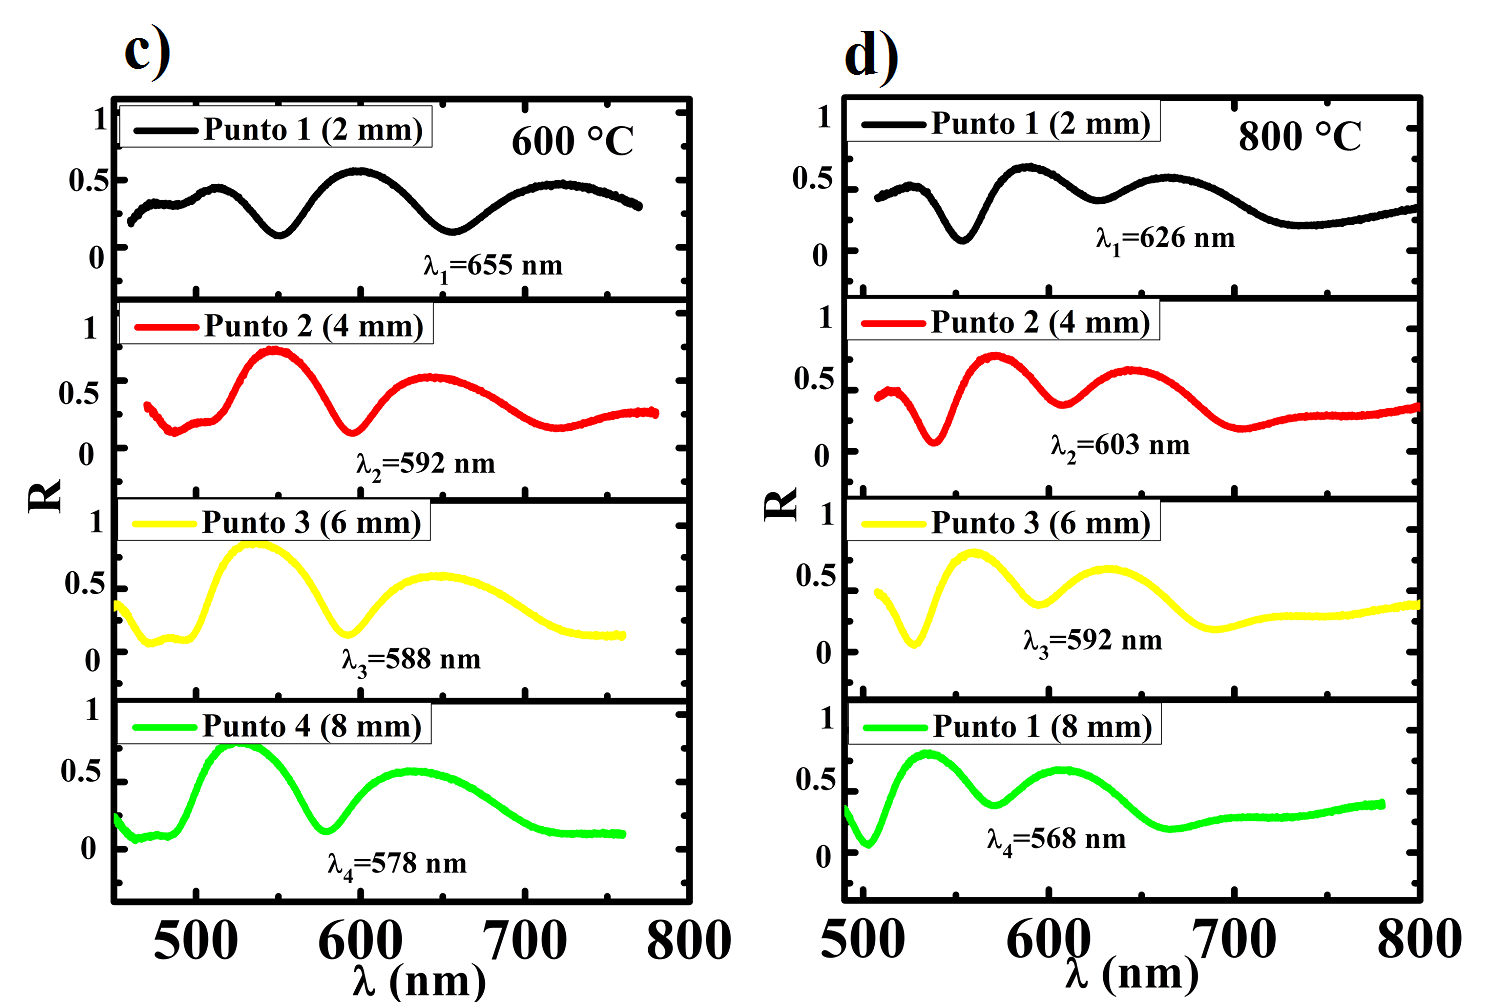
\includegraphics[scale=.25]{../Images/pl2}
	\caption{\emph{Mostramos el espectro de reflectancias ($\%$) en función de la longitud de onda (nm), de las microcavidades de silicio poroso con anodización asimétrica que se separaron electroquimicamente con disolvente,  se transfiere mecánicamente a cuarzo (MCL) y al final se le dio tratamiento térmico, como se indica en la Figura \ref{fig:p7}. a)  $21 ^{\circ} C$ para $MCL_{_{21^{\circ} C}}$ en el punto 1 ($\lambda_{_{1}}=681 nm$), punto 2 ($\lambda_{_{2}}=670 nm$), punto 3 ($\lambda_{_{3}}=668 nm$) y punto 4 ($\lambda_{_{4}}=644 nm$). b) $300^{\circ} C$ para $MCL_{_{300^{\circ} C}}$, $\lambda_{_{1}}=626 nm$,  $\lambda_{_{2}}=621 nm$,  $\lambda_{_{3}}=595 nm$ y $\lambda_{_{4}}=568 nm$. c) $600^{\circ} C$ para la muestra $MCL_{_{600^{\circ} C}}$, $\lambda_{_{1}}=655 nm$,  $\lambda_{_{2}}=592 nm$,  $\lambda_{_{3}}=588 nm$ y  $\lambda_{_{4}}=578 nm$. d) $800^{\circ} C$ para  $MCL_{_{800^{\circ} C}}$, $\lambda_{_{1}}=626 nm$, $\lambda_{_{2}}=621 nm$,  $\lambda_{_{3}}=595 nm$ y $\lambda_{_{4}}=568 nm$. }}
	\label{fig:p8}
\end{figure}

En la Figura \textbf{\ref{fig:p8} a)}  mostramos los espectros de reflectancia($\%$) en función de la longitud de onda (nm), que fueron sometidas a tratamiento térmico de $21^{\circ} C$ para $MCL_{_{21^{\circ} C}}$, como lo indica también la Figura \ref{fig:p7} a),  en el punto 1 ($\lambda_{_{1}}=681 nm$), punto 2 ($\lambda_{_{2}}=670 nm$), punto 3 ($\lambda_{_{3}}=668 nm$) y punto 4 ($\lambda_{_{4}}=644 nm$). Y medidos los anchos medios de los picos FWHM en cada punto de medición  20.1 nm (Para en punto 1),  21.4 nm (Para en punto 2),  18.9 nm (Para en punto 3) y  18.8 nm (Para en punto 4). Pasamos a la Figura \textbf{\ref{fig:p8} b)}  mostramos los espectros de reflectancia  con tratamiento térmico de $300^{\circ} C$ para $MCL_{_{300^{\circ} C}}$, como se observa en la la Figura\textbf{ \ref{fig:p7} b)}  en el punto 1 ($\lambda_{_{1}}=626 nm$), punto 2 ($\lambda_{_{2}}=621 nm$), punto 3 ($\lambda_{_{3}}=595 nm$) y punto 4 ($\lambda_{_{4}}=568 nm$). Y  los  FWHM  para cada punto de medición son  20.3 nm ,  19.5 nm ,  18.5 nm  y  19.2 nm respectivamente. En la siguiente la Figura \textbf{\ref{fig:p8} c)}  los espectros de reflectancia con tratamiento térmico de $600^{\circ} C$ para la muestra $MCL_{_{600^{\circ} C}}$  en los  puntos (1, 2, 3 y 4), visto en la la Figura \ref{fig:p7} c),  $\lambda_{_{1}}=655 nm$,  $\lambda_{_{2}}=592 nm$,  $\lambda_{_{3}}=588 nm$ y  $\lambda_{_{4}}=578 nm$ y los FWHM  en cada punto de medición son 29.3 nm ,  27.4 nm ,  28.1 nm  y  27.6 nm en el mismo orden. Y al final medimos en  la Figura \textbf{\ref{fig:p8} d)} mostramos las reflectancias de la muestra levantada y  con tratamiento térmico de $800^{\circ} C$ para  $MCL_{_{800^{\circ} C}}$ en los  puntos (1, 2, 3 y 4), así como se ve en la Figura \ref{fig:p7} d), $\lambda_{_{1}}=626 nm$, $\lambda_{_{2}}=621 nm$,  $\lambda_{_{3}}=595 nm$ y $\lambda_{_{4}}=568 nm$  y los FWHM  en cada punto de medición son 20.3 nm ,  19.5 nm ,  18.5 nm  y  19.2 nm  respectivamente.

\begin{table}[H]
	\begin{center}
		\begin{tabular}{|m{0.4cm}|  m{.8cm}| m{1cm} | m{1cm} | m{1.1cm} | m{1cm} | m{1.2cm} | m{1cm} |  m{1.2cm} |}
			\hline
			\multicolumn{9}{ |c| }{\textbf{FWHM (nm)}} \\ \hline
			\textbf{Pts} & {\tiny \textbf{MC}$_{_{21^{\circ} C}}$ }  & {\tiny  \textbf{MCL}$_{_{21^{\circ} C}}$} & {\tiny  \textbf{MC}$_{_{300^{\circ} C}}$ } & {\tiny \textbf{MCL}$_{_{300^{\circ} C}}$ }& {\tiny \textbf{MC}$_{_{600^{\circ} C}}$ } & {\tiny \textbf{MCL}$_{_{600^{\circ} C}}$} & {\tiny \textbf{MC}$_{_{800^{\circ} C}}$} & {\tiny \textbf{MCL}$_{_{800^{\circ} C}}$ }\\ \hline
			\textbf{1} &  22.1 & 20.1 & 19.2 & 20.3 & 20.5 & 29.3 & 28.4 & 32.2 \\ \hline
			\textbf{2} &  23.2 & 21.4 & 16.5 & 19.5 & 19.5 & 27.4 & 26.3 & 31.5 \\ \hline
			\textbf{3} &  19.4 & 18.9 & 17.9 & 18.5 & 20.9 & 28.1 & 27.5 & 30.7 \\ \hline
			\textbf{4} &  19.8 & 18.8 & 17.8 & 19.2 & 21.7 & 27.6 & 25.2 & 29.7 \\ \hline
			\multicolumn{9}{ |c| }{\textbf{Pts:} Puntos, \textbf{MC:} Microcavidad, \textbf{MCL:} Microcavidad Levantada} \\ \hline
		
		\end{tabular}
		\caption{\emph{Análisis el FWHM en función de la temperatura para cada pico de las microcavidades. El  FWHM  (Full Width at Half Maximum) se   denota $\Delta \lambda_{_{i}}  $  que describe  el ancho de pico correspondiente a la resonancia en $\lambda_{_{i}}$, para i=1,2,3,4. La temperatura se mide en ($^{\circ} C$) utilizada en el tratamiento térmico para cada una de las  muestras MC y MCL (para 21\grad C ,  300\grad C ,  600\grad C ,  800\grad C)}}
		\label{tab:t1}
	\end{center}
\end{table}
De las Figuras \textbf{\ref{fig:p4}} y \textbf{\ref{fig:p8} } se sacaron y  analizaron los espectros de reflectancias de cada una de las  muestras MC y MCL (para 21\grad C ,  300\grad C ,  600\grad C ,  800\grad C), en diferentes puntos (1(2mm), 2(4mm), 3(6mm) y 4(8mm)) y la tabla \ref{tab:t1}  nos muestras todos los FWHM en función de la temperatura para cada pico de las microcavidades fabricadas. Los  cambios observados es debido a la formación de dióxido de silicio ($SiO_2$); este cambio de longitud de onda muestra en diferentes  tiempos de oxidación y temperatura
\section{Conclusión}
El montaje y diseño de las microcavidad (MC) de silicio poroso con anodización asimétrica (AA) en solución acuosa y método de anodizacón es sencillo y económico. Igual que la  separación  electroquimicamente con disolvente, luego se transfiere mecánicamente a cuarzo (MCL) de dichas estructuras fotónicas. Se hizo una comparación de diferentes oxidaciones térmicas ( 21\grad C ,  300\grad C ,  600\grad C ,  800\grad C ),  encontrando  respuesta óptica en diferentes puntos de medición en el IR y el visible en una sola muestra alcanzando corrimiento de picos  $\Delta \lambda \sim \ \ 68 \ \ a \ \ 127 \ \ nm $. Se establecieron parámetros para calcular el FWHM encontrando como mínimos 16.5 nm y máximos 32.2 nm, como se observa en la tabla \ref{tab:t1}.  Es el primer reporte donde se compara diferentes  oxidación térmica en una sola  muestra de silicio poroso  con anodización asimétrica, sin levantar y levantada. 


\chapter{Modelo Electrostático para Cristales Fotónicos con Índices de Refracción con Gradiente (MECFGRIN) }
\label{Mo:MECFGRIN}
\markboth{CAPÍTULO 4. Modelo Electrostático para Cristales...}{}
\section{Introducción}
En esta parte queremos calcular  la densidad de corriente en una estructura GRIN producida por un ataque electroquímico sobre Si para producir Si poroso con una porosidad dependiente de la posición debido a la distancia al contraelectrodo. A simplifica el cálculo simplemente con la geometría.
Suponga un electrolítico todo con la forma de un prisma de los lados a, b, c con a, b horizontal y c vertical. Tomaré c como la altura del líquido. Las paredes son aislantes, pero el fondo está completamente cubierto por la muestra,  supongo que es un buen conductor. El electrodo es un cable aislado delgado pero para la punta, que considero una fuente puntual de corriente.
\begin{figure}[H]
	\centering
	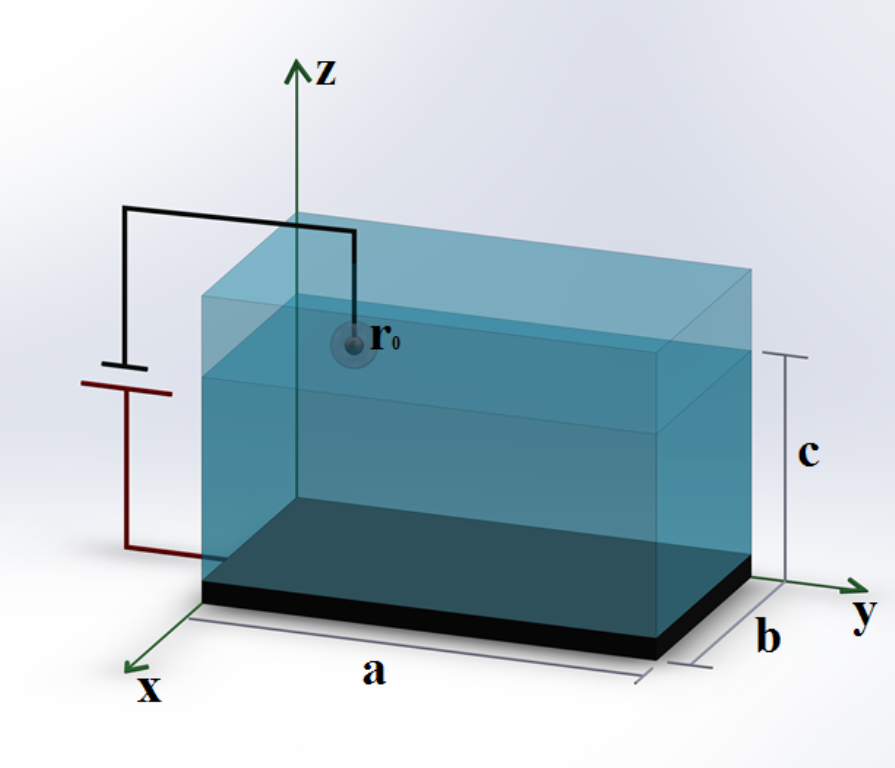
\includegraphics[scale=.4]{../Images/celdan} 
	\caption{\emph{ Esquema de la celda Electrolítica donde podemos ver la forma de un prisma de los lados a, b, c con a, b horizontal y c vertical. Tomaré c como la altura del líquido. Las paredes son aislantes, pero el fondo está completamente cubierto por la muestra,  supongo que es un buen conductor. La punta del electrodo es un cable aislado delgado que se ubica en el $\vec{r}_0$.}}
\end{figure}
La corriente en el electrólito es
\begin{equation}
\vec{j} = \sigma \vec{E}
\end{equation}
con $\sigma$ es la conductividad. Esto para el caso estacionario
\begin{equation}
\bigtriangledown \cdot \vec{j} = 0
\end{equation}
El campo eléctrico es derivado del potencial eléctrico,
\begin{equation}
\vec{E} =-\bigtriangledown \varphi	
\end{equation}
Y podemos decir que
\begin{equation}
\bigtriangledown^{2} \varphi=0	
\end{equation}
ya que la muestra es un conductor relativamente bueno, al conectarlo a tierra
\begin{equation}
\varphi(x,y,0)=0	
\end{equation}
Integrando $\vec{j}$ sobre una pequeña esfera superponiendo el electrodo se obtiene 

\begin{equation}
\int ds \cdot \vec{j} = I  	
\end{equation}
La densidad de corriente que lleva la corriente a la punta. Así
\begin{equation}
\int ds \cdot \vec{E} = \dfrac{I}{\sigma} 	
\end{equation}
El problema a resolver es así, obtener el potencial producido por una carga puntual

\begin{equation}
q_{_{0}} = \dfrac{I}{4 \pi \sigma} 	
\end{equation}
En las posiciones $\vec{r}_{_{0}}=(x_{_{0}}, y_{_{0}}, z_{_{0}})$ de la punta en presencia de un plano conductor a tierra $z=0$  y no conductor las paredes en  $(0, y ,z)$, $(a, y ,z)$, $(x, 0 ,z)$, $(x, b ,z)$ y la superficie del liquido también es no conductor  $(x, y ,c)$ la corriente normal es $\vec{j} \cdot \hat{n}=0$ y la normal del campo es
\begin{equation}
\vec{E} \cdot \hat{n}=0 	
\end{equation}
Es decir
\begin{equation}
E_{_{x}}(0, y ,z)= E_{_{x}}(a, y ,z)=E_{{_y}}(x, 0 ,z)=E_{{_y}}(x, b ,z)=E_{{_z}}(x, y ,c)=0
\end{equation}
 Esto tiene una mezcla de condiciones de contorno  tipo Dirichlet-Neumann. Al usar la geometría de prisma simplificada puedo resolver el problema usando la teoría de las cargas imágenes. Cada carga tiene una imagen de mismo signo y magnitud para cada superficie aislante lateral  y el cambio  de signo opuesto en la parte inferior del plano conductora, es decir hacia abajo. 
\begin{figure}[H]
	\centering
	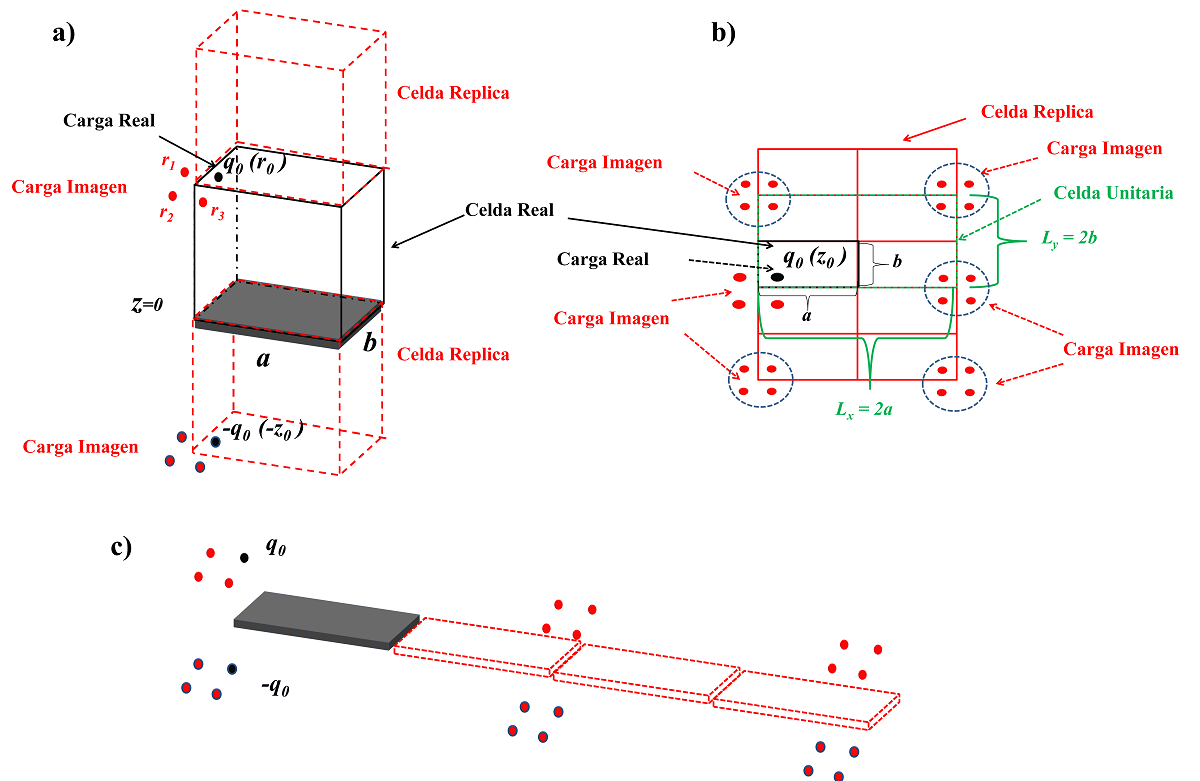
\includegraphics[scale=.42]{../Images/Cellgrin}
	\caption{\emph{a)Esquema de una celda electrolítica rectangular, con una carga real en la esquina de la celda con sus cargas ($q$) imágenes de  igual signo en $Z_0$ y otra carga imagen ($-q$) con cambio de signo  ubicada debajo del  conductor en la posición $-Z_0$. b)La cara superior vista desde arriba, una carga real y sus cargas imágenes  en el $Z_0$. c) Todo esto formado un  sistemas de una carga real y sus  cargas imágenes producidas por las paredes de la celda y sus otras imágenes  vista desde arriba, formando un espacio periódicos. }}
	\label{fig:T1}
\end{figure}
De la Figura \textbf{\ref{fig:T1}} suponemos que si pongo una carga real ($q$) en $\vec{r}_0= (x_0, y_0, z_0)$, en la esquina de la celda electrolítica induce imágenes en $\vec{r}_1= (-x_0, y_0, z_0)$ debido a un reflejo en $(0, y, z)$, imágenes en $\vec{r}_2= (-x_0, -y_0, z_0)$ debido a un reflejo en  $(x, 0, z)$ y la imagen de la imagen en $\vec{r}_3= (x_0, -y_0, z_0)$  para $\vec{r}_j$, $(j=0,1,2,3)$. Luego, estas cuatro cargas se reflejan en las otras dos superficies y las ocho nuevas imágenes se reflejan en la superficie original, etc., produciendo una red rectangular 2D periódica con celdas unitarias de signos  $L_x=2a$ , $L_y=2b$ y con una base de 4 cargas iguales. Toda esta red se refleja por la parte inferior con una carga de signo opuesta (abajo del conductor). Las copias periódicas separadas por el vacío en el plano $xy$ cuya área se está incrementando para lograr la convergencia. \\
\textbf{Consideraciones del problema }:  El problema es del potencial, el campo y la corriente producida por una red periódica 2D de una carga real y todas sus imágenes. El potencial debido a una red periódica se encuentra de forma automática en el plano haciendo una suma de Fourier 2D.  
\begin{eqnarray}
\rho(\vec{r}) =q \displaystyle\sum_{R}  \ \delta (\vec{r}-\vec{R}-\vec{r}_0) =\dfrac{q}{A}  \displaystyle\sum_{G}  e^{i G \cdot (\vec{r}-\vec{r}_{0})} \delta (z-z_0)
\end{eqnarray}
Donde ${R}$ es la red 2D Bravais y ${G}$ su red recíproca. Se escribe

\begin{eqnarray}
\phi(\vec{r}) = \displaystyle\sum_{\vec{G}} \phi_{_{G}} (z) e^{i \vec{G} \cdot \vec{r}}
\end{eqnarray}

De modo que la ecuación de Poisson
\begin{eqnarray}
\bigtriangledown^2 \phi=-4 \pi \displaystyle\sum_{\vec{R}} \delta (\vec{r}-\vec{R}-\vec{r}_0)
\end{eqnarray}

Se convierte
\begin{eqnarray}
\dfrac{\partial^2 \phi_{_{G}}(z)}{\partial z^2}+ G^2\phi_{_{G}}(z)= -\dfrac{4 \pi}{A}  q   e^{i \vec{G} \cdot \vec{r}_{_0}} \delta (z-z_0)
\end{eqnarray}
Resolviendo la ecuación homogénea arriba y abajo $ z = z_0 $, usando simetría y condiciones en $\pm \infty $ obtenemos

\begin{eqnarray}
\phi_{_{G}}= \phi_{_{G}}^{0}  e^{ G \abs{z-z_0}} \ \ \ \ \ (G\neq 0)
\end{eqnarray}
Y ajustando la singularidad

\begin{eqnarray}
\phi_{_{G}}(z)= \dfrac{2 \pi q}{AG}  e^{- G \abs{z-z_0}} e^{-i \vec{G} \cdot \vec{r}_{_0}} \ \ \ \ \ (G\neq 0)
\end{eqnarray}
Para el caso $G=0$ es similar 
\begin{eqnarray}
\phi_{_{G=0}}(z)= \dfrac{-2 \pi q}{A}  \abs{z-z_0} +K, 
\end{eqnarray}
K es una constante. Aquí $ A = L_x L_y $ es el área de celda unitaria

\begin{eqnarray}
\phi(\vec{r}) = K-\dfrac{2 \pi q}{A}  \abs{z-z_0} +\dfrac{2 \pi q}{A}\displaystyle\sum_{\vec{G}} \dfrac{1}{G} e^{- G \abs{z-z_0}}   e^{i \vec{G} \cdot \vec{r}-\vec{r}_0}
\end{eqnarray}
Adicionando todas las cargas  imágenes,
\begin{eqnarray}
\nonumber \phi(\vec{r}) = -\dfrac{8\pi q}{A} \bigg((\abs{z-z_0}-\abs{z+z_0} ) +\dfrac{8\pi q}{A}\displaystyle\sum_{\vec{G}} \dfrac{1}{G} \bigg( e^{- G \abs{z-z_0}} e^{- G \abs{z+z_0}}  \bigg) \\ \cos(G_x x_0) \cos(G_y y_0) e^{i \vec{G} \cdot \vec{r}} \ \ \ \
\end{eqnarray}

A una altura $ 0<z<z_0 $ simplifico
\begin{eqnarray}\label{Eq:EC11}
\phi(\vec{r}) = -\dfrac{16\pi q}{A} \bigg( z +\displaystyle\sum_{\vec{G}} \dfrac{1}{G} \sinh(G z)  \cos(G_x x_0) \cos(G_y y_0) e^{i \vec{G} \cdot \vec{r}} \bigg)
\end{eqnarray}

Si la superficie del líquido está a una altura finita c, entonces puedo usar imágenes, como:
\begin{figure}[H]
	\centering
	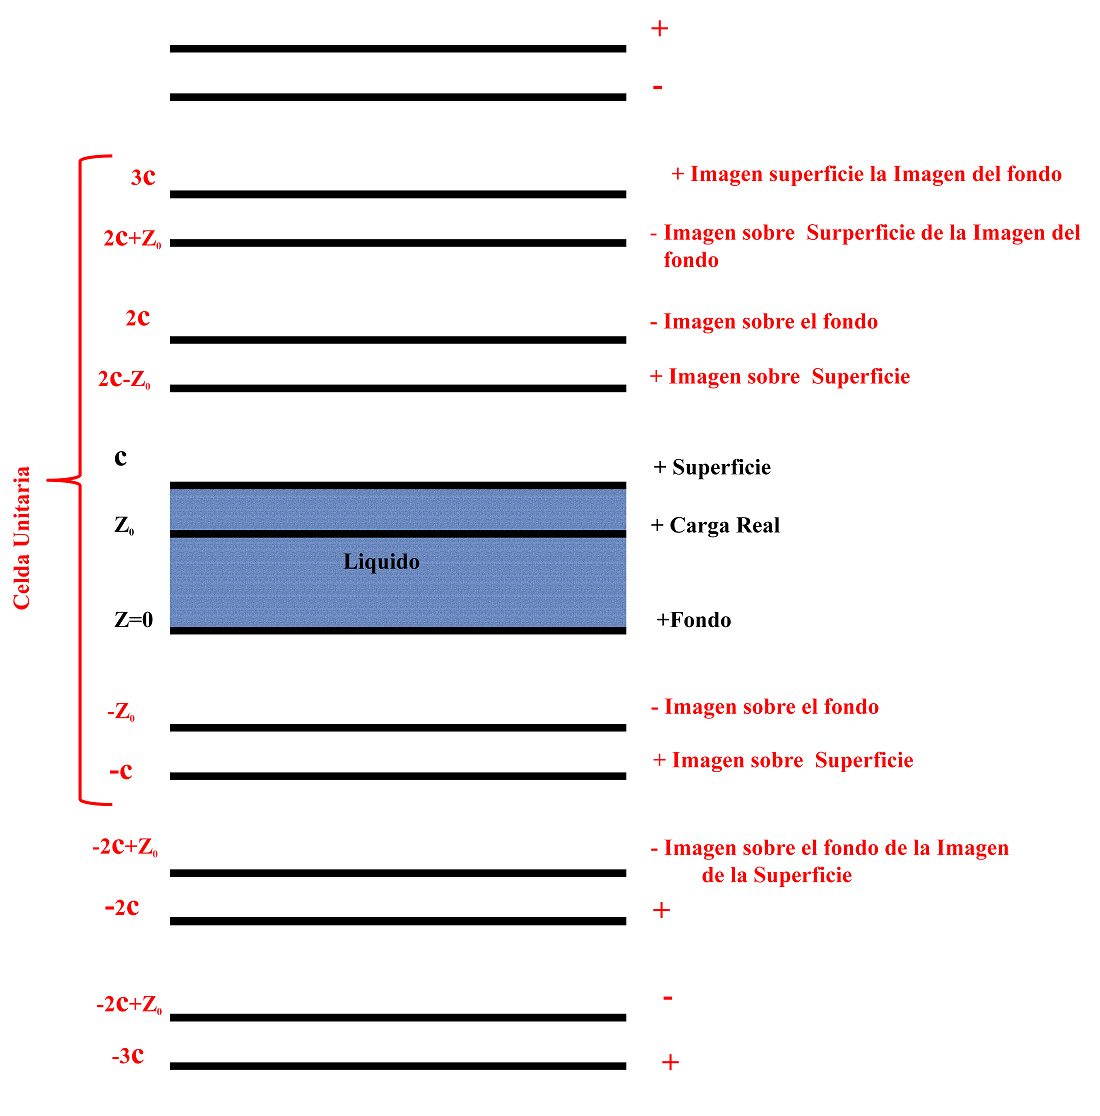
\includegraphics[scale=.35]{../Images/celd1}
	\caption{\emph{Diagrama donde se observa que hay un plano positivo (real) $ z_0 $, una imagen negativa a $ -z_0 $ debajo del conductor($z=0$)  y sus imágenes son una placa positiva a $ 2c-z_0 $ y una placa negativa a $ 2c + z_0 $, la imagen se repite  verticalmente con el período $ L_z = 4c $}}
\end{figure}
Observe que hay un plano positivo (real) $ z_0 $, una imagen negativa a $ -z_0 $ debajo del conductor ($z=0$) y sus imágenes son una placa positiva a $ 2c-z_0 $ y una placa negativa a $ 2c + z_0 $. Además, la imagen se repite  verticalmente con el período $ L_z = 4c $. Por lo tanto, la ecuación  \ref{Eq:EC11} se  reescribiría, así
{\small 
\begin{eqnarray}\label{Eq:EC12}
\nonumber\phi(\vec{r}) = K+\dfrac{8\pi q}{A} \displaystyle\sum_{n} -\bigg(\abs{z-z_0-nL_z}-\abs{z+z_0-nL_z}-\abs{z+2c+z_0-nL_z}+ \\ \nonumber \abs{z-2c-z_0-nL_z}\bigg) +  \dfrac{1}{G}\displaystyle\sum_{\vec{G}}\bigg( \displaystyle\sum_{n} \bigg( e^{-\abs{z-z_0-nL_z}} +e^{-\abs{z+z_0-nL_z}}\\ \nonumber -e^{-\abs{z+2c+z_0-nL_z}}-e^{-\abs{z-2c-z_0-nL_z}}  \bigg)\bigg)\cos(G_x x_0) \cos(G_y y_0) e^{i \vec{G} \cdot \vec{r}}\\
\end{eqnarray}
}
La constante K se elige así $ \phi(z=0)$

\begin{equation}
\abs{z-z_0-nL_z}= \left\lbrace
\begin{array}{ll}
z-z_0-nL_z \Rightarrow \ \ n<0 \\\\
-z+z_0-nL_z \Rightarrow \ \ n\geq 0
\end{array}
\right.
\end{equation}
\begin{equation}
\abs{z+z_0-nL_z}= \left\lbrace
\begin{array}{ll}
z+z_0-nL_z \Rightarrow \ \ n <0 \\\\
-z-z_0+nL_z \Rightarrow \ \ n\geq 0
\end{array}
\right.
\end{equation}

\begin{equation}
\abs{z+2c+z_0-nL_z}= \left\lbrace
\begin{array}{ll}
z-2c+z_0-nL_z \Rightarrow \ \ n <0 \\\\
-z+2c-z_0-nL_z \Rightarrow \ \ n\geq 0
\end{array}
\right.
\end{equation}

\begin{equation}
\abs{z-2c+z_0-nL_z}= \left\lbrace
\begin{array}{ll}
-z-2c-z_0+nL_z \Rightarrow \ \ n <0 \\\\
z+2c+z_0-nL_z \Rightarrow \ \ n\geq 0
\end{array}
\right.
\end{equation}

Substituyendo en la ecuación \ref{Eq:EC12} los campos 
\begin{eqnarray}
\nonumber\phi(\vec{r}) = K+\dfrac{8\pi q}{A} \bigg(  2z+2z_0  +2 \displaystyle\sum_{n}\dfrac{1}{G}\bigg(e^{-Gz_0} \\  \nonumber\sinh(Gz)+e^{-Gz_0(2c_z-z)} \sinh(Gz)\bigg) \times \cos(G_x x_0) \\  
\nonumber \cos(G_y y_0) e^{i \vec{G} \cdot \vec{r}} + 2\dfrac{1}{G}\displaystyle\sum_{\vec{G}}  \displaystyle\sum^{\infty}_{n=1}\bigg(   e^{-G(-z-z_0+nL_z)} \\  \nonumber +e^{-G(z-z_0+nL_z)}-e^{-G(-z-z_0+nL_z)}  +e^{-G(z+z_0+nL_z)}+ \\  \nonumber e^{-G(-z-2c+z_0-nL_z)}+ e^{-G(-z-2c-z_0-nL_z)}  - e^{-G(-z-2c-z_0+nL_z)} \bigg) \\  \nonumber \times \cos(G_x x_0) \cos(G_y y_0) e^{i \vec{G} \cdot \vec{r}} \bigg)\\
\end{eqnarray}
Y que se convierte, después de factorizar $ e ^ {- nGL_Z}$ y hacer explícitamente la suma geométrica sobre n

\begin{eqnarray}\label{Eq:EC13}
\nonumber\phi(\vec{r}) = K+\dfrac{16\pi q}{A} \bigg(z+z_0  + \displaystyle\sum_{\vec{G}}\dfrac{1}{G}  \\ \nonumber\bigg(e^{-Gz_0} \sinh(Gz)+e^{-Gz_0(2c_z)} \sinh(Gz_0) -e^{-2Gc} \sinh(Gz) \sinh(Gz_0) \\ \nonumber \dfrac{1+\cosh(2Gc)}{\sinh(2Gc)} - e^{-2Gc}\cosh(2Gc) \sinh(Gz_0)   \bigg) \cos(G_x x_0) \cos(G_y y_0) e^{i \vec{G} \cdot \vec{r}}   \bigg)\\
\end{eqnarray}
Evaluando para $ z = 0 $
{\small
\begin{eqnarray}
\nonumber\phi(x, y, 0) = K+\dfrac{16\pi q}{A} \bigg(z_0  + \displaystyle\sum_{\vec{G}}\dfrac{1}{G}  \\ \nonumber\bigg(e^{-2Gc} \sinh(Gz_0)-e^{-2Gc} \sinh(Gz_0)   \bigg) \cos(G_x x_0) \cos(G_y y_0) e^{i \vec{G} \cdot \vec{r}} = K+\dfrac{16\pi q}{A} \bigg)\\
\end{eqnarray} }
Independiente de $ x $ y $ y $ para poder configurar
\begin{eqnarray}
K=\dfrac{16\pi q}{A} 
\end{eqnarray}
Puedo simplificar aún más la ecuación \ref{Eq:EC12} para obtener
\begin{eqnarray}
\nonumber\phi(\vec{r}) = \dfrac{16\pi q}{A}\bigg( z  + \displaystyle\sum_{\vec{G}}\dfrac{\sinh(Gz_0)}{G}  \\ \nonumber\bigg(e^{-Gz_0} -e^{-3Gc} \dfrac{\cosh(Gc)\sinh(Gz_0)}{\sinh(2Gc)}   \bigg) \cos(G_x x_0) \cos(G_y y_0) e^{i \vec{G} \cdot \vec{r}}  \bigg)\\
\end{eqnarray}
Estoy seguro de que es correcto. Dpes va a cero en $ z = 0 $. El término con c desaparece si $ c \longrightarrow \infty $. La suma converge como $ G\longrightarrow \infty $ si $ z< z_0 < c $ y diverge a $ z \longrightarrow z_0 $. Por lo tanto, parece listo para el cálculo.
La componente normal del campo es
\begin{eqnarray}
\nonumber E_\perp = -\dfrac{16\pi q}{A}\bigg( 1  + \displaystyle\sum_{\vec{G}}\dfrac{1}{G} \cosh(Gz) \\ \nonumber\bigg(e^{-Gz_0} -e^{-3Gc} \dfrac{\cosh(Gc)\sinh(Gz_0)}{\sinh(2Gc)}   \bigg) \cos(G_x x_0) \cos(G_y y_0) e^{i \vec{G} \cdot \vec{r}}  \bigg)\\
\end{eqnarray}
Y la densidad de corriente 
\begin{eqnarray}\label{Eq:J}
\nonumber j_\perp = -\dfrac{I}{ab}\bigg( 1  + \displaystyle\sum_{\vec{G}}\dfrac{1}{G} \cosh(Gz) \\ \nonumber\bigg(e^{-Gz_0} -e^{-3Gc} \dfrac{\cosh(Gc)\sinh(Gz_0)}{\sinh(2Gc)}   \bigg) \cos(G_x x_0) \cos(G_y y_0) e^{i \vec{G} \cdot \vec{r}}  \bigg)\\
\end{eqnarray}
Integrando sobre la superficie de la muestra se obtiene 
\begin{eqnarray}
\nonumber I_{nm} =\int^{a}_0 dx \int^{b}_0 dy \ \ e^{i\vec{G}\vec{r}}=\dfrac{1}{G_x G_y} (e^{-iG_xa}-1) (e^{-G_y b}-1) \\ =\dfrac{ab}{nm \pi^2} ((-1)^n-1-1)(-(1)^m-1-1)
\end{eqnarray}
Usando el factor del vector reciproco de esta forma.
\begin{eqnarray}
\vec{G}=\bigg(\dfrac{\pi}{a}n,\dfrac{\pi}{b}m\bigg)\lim
\end{eqnarray}
sin embargo, como todos los coeficientes de $ e^{- i \vec{G} \vec{r}} $ en (32) son pares en $ \vec{G} $ y la integral es impar en n y m, solo el contribuyente a término constante a la corriente integrada
\begin{eqnarray}
\nonumber I^{nm} =\int \vec{J} dx  dy =-\int \vec{J}_\perp dx  dy=\dfrac{I}{ab}\int dx \int dy=I
\end{eqnarray}
\section{Simulación del modelo MECFGRIN}
Para probar la idea desarrollada en la sección teórica, encontramos una relación de la punta del contraelectrodo que actúa análogamente como una carga puntual y la densidad de corriente para una geometría en una caja electrolítica y resolvemos las ecuaciones electrostática con condiciones de contornos adecuadas. Dando como resultado un modelo electrostático para cristales fotónicos con índice de refracción con gradiente (MECFGRIN), del capitulo \ref{Mo:MECFGRIN}
\begin{figure}[H]
	\centering
	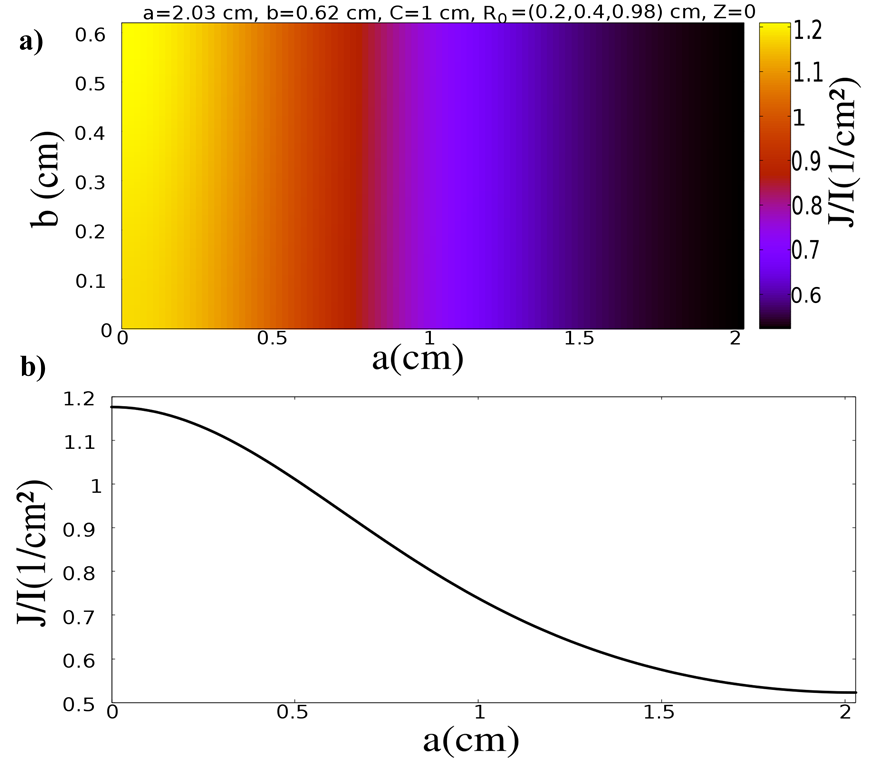
\includegraphics[scale=0.45]{../Images/G123}
	\caption{\emph{Simulación para calcular la densidad de corriente en una estructura con índice de refracción de gradiente (GRIN) producida por ataque  electroquímico en silicio cristalino  para producir de silicio poroso (SiP), con un perfil de densidad de corriente $J(mA/cm^2) $ normalizado con la corriente eléctrica $I(mA)$, nos queda $J/I \sim 0.5 \ \ a \ \ 1.2 (1/cm^2) $, para una celda de $a=2.03 \ \ cm $ y $b= 0.62 \ \ cm$, con una altura del electrodo $Z_0 =0.96 \ \ cm$} Ec. (\textbf{\ref{Eq:J}})}.
	\label{fig:DR1}
\end{figure} 
Consideramos la Figura \textbf{\ref{fig:DR1}}  que salen de resolver la Ecuación (\textbf{\ref{Eq:J}}), calculando la densidad de corriente en función del área de la  celda rectangular  de $1.206\ \ cm^2 $, la programación la hicimos con el paquete de PDL de PERL y Graficamos en gnuplot. Optimizamos los valores adecuado para que nuestra densidad de corriente atacara adecuadamente al silicio cristalino, dando el efecto de gradiente. Utilizamos como largo $a=2.03\ \ cm$ y ancho $b=0.62\ \ cm$ la altura de la solución esta $c=1\ \ cm$ y pudimos ubicar la punta del electrodo en $R_0 =(X_0=0.2,\ \ Y_0=0.4 \ \ , Z_0=0.96) \ \ cm$ y evaluado en la superficie sobre la interfaz del silicio, en el plano $Z=0$. En esta misma Fig. \textbf{\ref{fig:DR1}}, obtenemos  un perfil de densidad de corriente $J(mA/cm^2) $ normalizado con la corriente eléctrica $I(mA)$, nos queda $J/I \sim 1.2 \ \ a \ \ 0.5 (1/cm^2) $, como lo vemos en la  Figura \textbf{\ref{fig:DR1} a)} un  efecto que sucede sobre la superficie de la muestra, un cambio de contrate debido a las diferentes densidades de corrientes atacadas. Vemos el comportamiento de decaimiento que tiene el perfil igual que  la Fig. \textbf{\ref{fig:DR1} b)} que es un corte sobre el eje de las $a$. Cuando Variamos las corrientes podemos observar el comportamiento de cambios de densidade de corriente normalizada, con los datos obtenidos por medio de la simulación pudimos tener una  mejor optimización en el diseño de silicio poroso proponiendo un nuevo y novedoso arreglo experimental, del mismo modo podemos darnos una idea por medio del gráfico de como  seria el ataque y la formal lateral de los poros en el silicio.\\ 
 En la Figura \textbf{\ref{fig:DR2}}, consideramos una corriente de $I=5\ \ mA$, obteniendo un perfil de densidad de corriente de $J\sim 6 \ \ a \ \ 2.5 (mA/cm^2) $, como lo vemos en la Fig. \textbf{\ref{fig:DR2} a)} un  efecto que sucede sobre la superficie de la muestra, un cambio de contrate debido a las diferentes densidades de corrientes atacadas. Para la Figura \textbf{ \ref{fig:DR2} b)}, vemos el comportamiento de decaimiento que tiene el perfil igual que la Fig. \textbf{\ref{fig:DR1} c)} que es un corte sobre el eje de las $a$. Cuando cambiamos la corriente $I= 40 \ \ mA$ encontramos que la densidad de corriente aumenta $J\sim 50 \ \ a \ \ 20 (mA/cm^2) $ como se ve en  la  Fig. \textbf{\ref{fig:DR2}}, teniendo las mismas consideraciones expuesta para la  Fig. \textbf{\ref{fig:DR1}} sobre como decae $J$.
\begin{figure}[H]
	\centering
	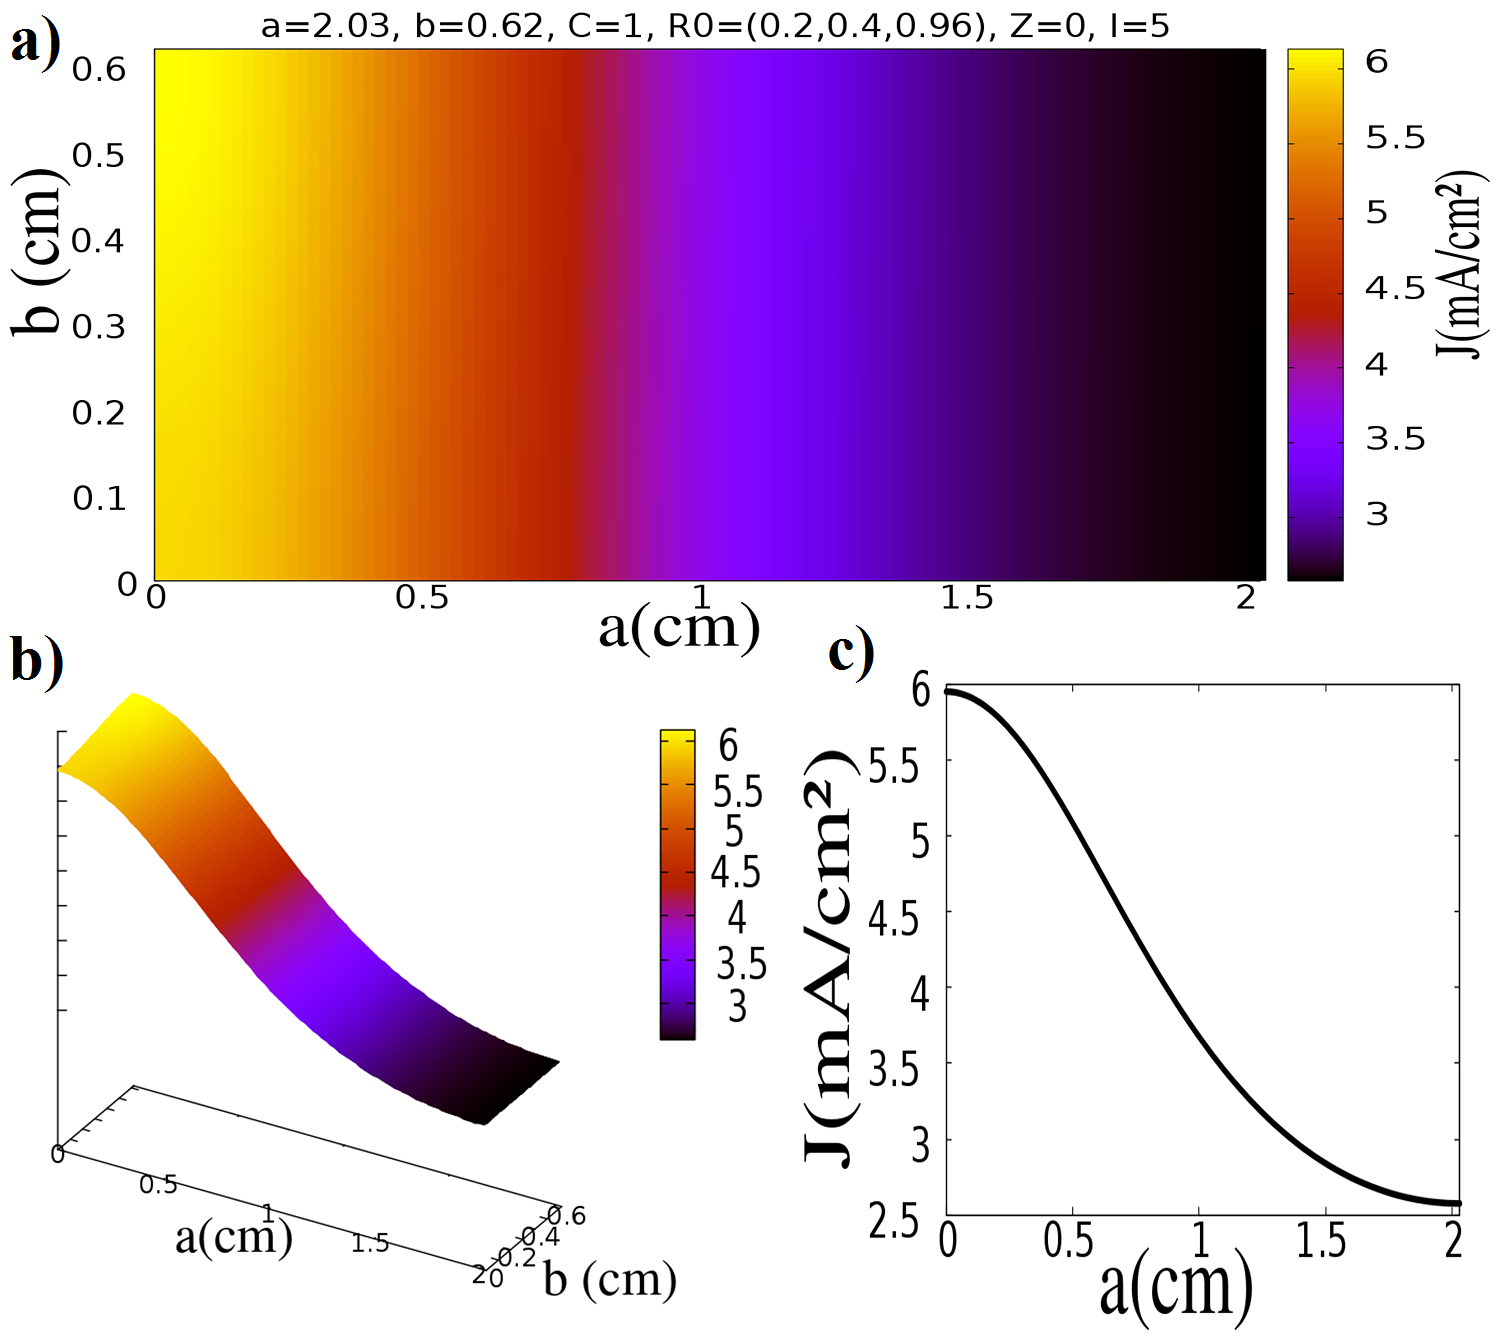
\includegraphics[scale=0.3]{../Images/j51}
		%\includegraphics[scale=0.3]{../Images/j40}
	\caption{\emph{Simulación para calcular la densidad de corriente en una estructura  (GRIN), teniendo en cuenta las consideraciones de  la Figura \textbf{\ref{fig:DR1}}. a) El caso cuando $I=5 mA$ nos da $J\sim 6 \ \ a \ \ 2.5 (mA/cm^2) $. b) Vemos el comportamiento de decaimiento que tiene el perfil sobre la Densidad de Corriente. c) Es un corte sobre el eje de las $a$ en función de J}}
	\label{fig:DR2}
\end{figure}
\chapter{Optimización de Silicio Poroso(SiP) con Índice de refracción con Gradiente (GRIN)}
\label{Mo:MODELOGRIN}
\markboth{CAPÍTULO 5. Optimización de Silicio Poroso(SiP)...}{}
\section{Resumen}
Se pudo calcular la densidad de corriente en una estructura GRIN producida por un ataque electroquímico en silicio (Si)  para obtener  silicio poroso (SiP) con una porosidad que depende de la posición debido a la distancia al contra electrodo. Encontramos una relación de la punta del contraelectrodo que actúa an\'alogamente como una carga puntual y la densidad de corriente para una geometr\'ia en una caja electrolítica y resolvemos las ecuaciones electrostática con condiciones de contornos adecuadas. Dando como resultado un modelo electrostático para cristales fotónicos con \'indice de refracción con gradiente (MECFGRIN). La caracterización de las estructuras de silicio se realizó mediante espectroscopia SEM  y UV-Vis-NIR . Estos resultados abren la posibilidad de crear estructuras fotónicas basadas en silicio dentro del rango IR-Visibles dentro de la misma muestra en diferentes distancia de medición, generando diferentes poros y porosidades. Luego del estos cálculos y de caracterizar las muestras de silicio poroso pudimos diseñar estructuras fot\'onicas  complejas como microcavidades \'opticas, controlando las densidades de corriente, las porosidades y los indices efectivos de dicha estructura. 
\section{Introducci\'on}
El comportamiento y la estructuras de los materiales nanoestructurados se ha convertido en un gran tema de interés mundial donde ha resultado numerosas  investigación desde hace algún tiempo.\cite{I1} Encontramos un gran camino por recorrer  para las futuras exploraciones tecnológicas, un sinnúmero de retos y desafíos que abre un abanico de posibilidades para desarrollar estudio mas avanzando sobre dichos temas.\cite{I2} El silicio poroso (SiP) es un material nanoestructurado versátil y un excelente candidato como plataforma tecnológica para diferentes aplicaciones de sensado.\cite{I3,I4} Esto último, gracias a su fácil fabricación, su grande área superficial, su alta reactividad de superficie, y sobre todo, por su capacidad de transducción óptica. Los cristales fotónicos  son estructuras multicapa dieléctricas que presentan periodicidad en la función dieléctrica a lo largo de una dirección.\cite{I5} Tiene numerosos  estudios por  alta reflectividad y la capacidad de ajuste de la banda prohibida fotónica (PBG)\cite{I6}, lo que lleva a posibles aplicaciones como filtros, \cite{I7} interruptores ópticos, \cite{I8} espejos omnidireccionales, \cite{I9} guías de onda para PC, \cite{I10}  etc.
En la fabricación convencional de SiP el resultado deseado es obtener muestras homogéneas (mismas características estructurales) desde la periferia hasta el centro del área atacada electroquímicamente.  En Trabajos previos que involucran la fabricación de muestras graduadas ( es decir, que muestran un gradiente estructural) emplean una configuración de anodización asimétrica, \cite{I101, I102, I103, I104} para formar películas de PS que exhiban esta característica. Sin embargo, con una configuración de anodización asimétrica se obtienen muestras con un gradiente lateral en términos de tamaño de poro y espesor de la capa porosa.\cite{I101} En esta configuración, la cara del electrodo de platino (cátodo) se mantiene relativamente perpendicular a la superficie del sustrato de Si (ánodo) en uno de los extremos de la celda, de tal forma que la distribución de la corriente dentro de la solución electrolítica varía en función de la distancia del electrodo debido a la resistencia del electrolito, resultando en una disminución de la densidad de corriente conforme la distancia desde el electrodo aumenta.\cite{I102,I103} El resultado es una superficie porosa con diferentes tamaños de poros que van desde unos cuantos nanómetros hasta poros del orden de unos cuantos micrómetros.\cite{I104} Las dimensiones de los poros obtenidos en el mismo chip pueden controlarse ajustando la corriente de anodización y la concentración del electrolito \cite{I11}. Actualmente, este tipo de muestras han encontrado relevante su aplicación como filtros de banda ópticos \cite{I12}, dispositivos con banda fotónica multidireccional (códigos de barra fotónicos) \cite{I13} y principalmente, como biosensores. De esta forma, se estudia el efecto que ejercen diferentes topografías (porosidades en la misma muestra) en el cultivo/adhesión de ciertas células \cite{I14} , reduciendo considerablemente la cantidad de muestras y costo del estudio. Además, también son muy útiles cuando se requiere una técnica de exclusión por tamaño de biomoléculas permitiendo la identificación y separación de estos compuestos biológicos \cite{I15}. Y estudios recientes demostraron que la combinación de oxidación térmica e infiltración de $TiO_2$ por ALD ofrece la oportunidad de fabricar un alto índice de refracción de contraste, elementos ópticos GRIN visiblemente transparentes a partir de estructuras absorbentes de SiP.\cite{I16}  A pesar de las investigaciones anteriores sobre la formación de silicio porosos con GRIN, tipo p en fabricación y caracterización, no se ha tenido un control en  las densidades de corriente en el ataque del silicio cristalino ni se había planteado un modelo detallado que explicará dicho gradiente lateral en la fabricación. 

\section{Detalles Experimentales}
\begin{figure}[H]
	\centering
	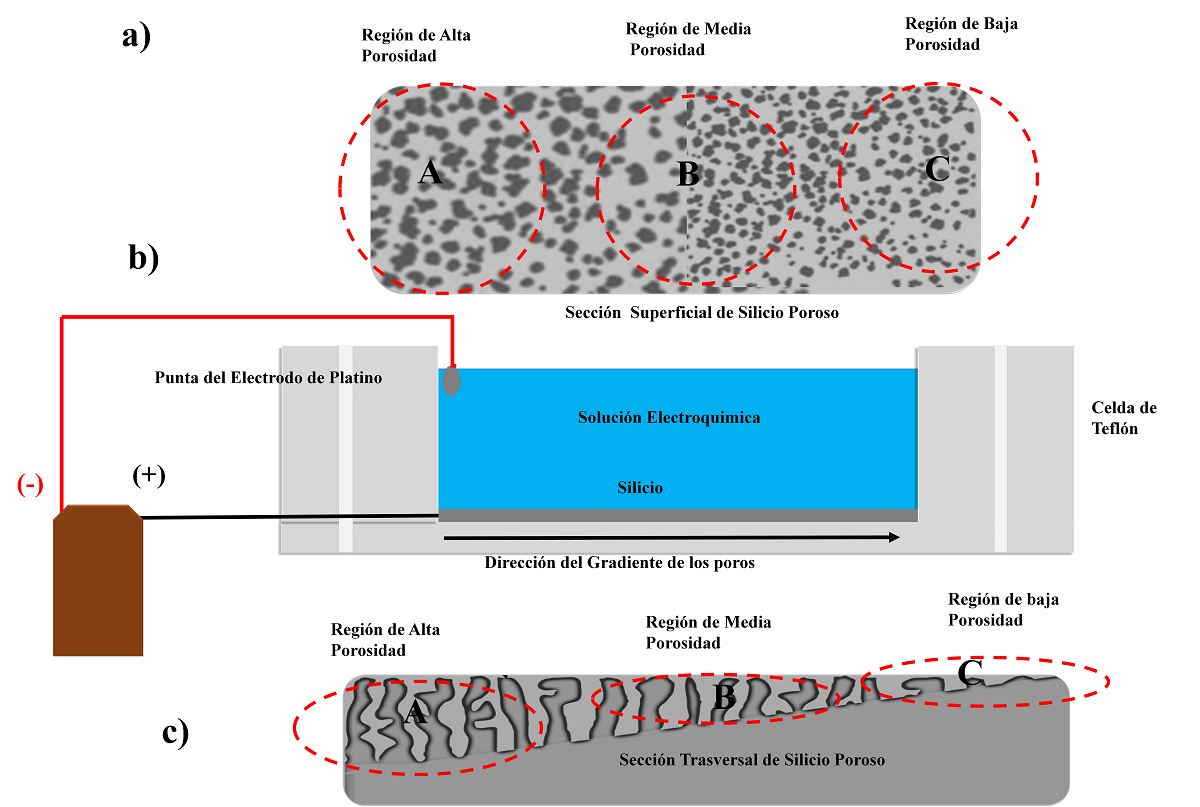
\includegraphics[scale=0.35]{../Images/DE1}
	\caption{\emph{Esquema del montaje experimental donde se puede fabricar silicio poroso con GRIN. a) Dibujamos en esquema de la sección superficial, divido por tres regiones A, B y C, de Alta, Media y Baja Porosidad. b) Es el esquema de la celda electroquímica con sus partes: oblea de silicio,  celda de teflón, electrodo de punto de platino, Solución Acuosa electroquímico y la conexión del circuito con el cátodo y ánodo. c) Es un dibujo del esquema de la sección Trasversal del silicio poroso atacado electroquímicamente vista en tres regiones diferente como se  menciono anteriormente. }}.
	\label{fig:DE1}
\end{figure}
La Figuras \textbf{\ref{fig:DE1}} se muestra un esquema del montaje experimental donde se puede fabricar silicio poroso con GRIN, teniendo en cuentas las consideraciones del electrodo como punta, la celda rectangular y la muestra(oblea de silicio) con mayor área de ataque rectangular.
En la Fig. \textbf{\ref{fig:DE1} a)} Dibujamos en esquema de  la sección superficial, divido por tres regiones A, B y C, de Alta, Media y Baja Porosidad. Todo esto correspondiente a lo que se espera obtener en los experimentos. La Fig. \textbf{\ref{fig:DE1} b)} Es el esquema  la celda electroquímica con sus partes: oblea de silicio,  celda de teflón, electrodo de punto de platino, Solución Acuosa electroquímico y la conexión del circuito con el cátodo y ánodo. Por ultimo la  Fig. \textbf{\ref{fig:DE1} c)} Es un dibujo del esquema de la sección Trasversal del silicio poroso atacado electroquímicamente vista desde  tres regiones diferente como se  menciono anteriormente. En la sección 3.1 damos los detalles utilizados para realizar nuestros experimentos.

\subsection{Fabricación de Monopeliculas de Silicio Poroso GRIN}
Algunas de las estructuras fotónicas simuladas se fabricaron mediante  anodización electroquímica sobre una oblea de Si cristalina de tipo p orientada (100) (resistividad 0.002 - 0.005 $ \Omega \cdot cm$), en condiciones galvanostáticas [14]. El proceso de anodización electroquímica se realizó a temperatura ambiente, con una mezcla electrolítica de HF acuoso (concentración: 48 $ \% $ de peso), glicerol (pureza: 99.8$ \% $ de peso) y etanol (pureza: 99.9$ \% $ de peso) en 3: 7 : 1 proporción de volumen, respectivamente. Después del proceso de anodización, las muestras se enjuagan con etanol (pureza: 99,9$ \% $ en peso).   El diseño de la celda usada  es de $1.206\ \ cm^2$ (esta es la superficie atacada en el proceso), el área atacada es de forma rectangular ($0.62\ \ cm \times 2.03 \ \ cm$ )  esto con el fin de que las densidades de corriente que ataca tenga un gradiente lateral. Fueron fabricadas con una corriente fija de $5 \ \  mA$ para generar  diferentes densidades de corrientes variando de  $6 \ \ mA/cm^2$ a $2.5 \ \ mA/cm^2$. De igual modo, utilizamos la corriente de $40 \ \  mA$  para general   $50\ \ mA/cm^2$ a $20\ \  mA/cm^2$.   El cátodo esta constituido de un alambre de platino que fue arreglado en forma de una punta de diámetro aproximado de ($0.5\ \ mm$). 
\subsection{Medición de la Reflectancia}
Las mediciones de reflectividad se llevaron a cabo con un espectrofotómetro UV-Vis-NIR Perkin Elmer Lambda 950, para la parte experimental. Para La parte teórica  se  calcula el índice de refracción complejo $ \tilde{n}_{_{SiP}} = n_{_ {SiP}} - ik_{_{SiP}} $ de una capa porosa con porosidad y espesor homogéneos con interfaces suaves a lo largo de toda la estructura, cuanto más adecuado sea medios es el procedimiento de ajuste de la reflectancia experimental o espectro de transmitancia. Para el caso del espectro de reflectancia, SiP puede realizar el procedimiento de ajuste para una sola capa lisa(monopelicula) \cite{I17, I18, I19}.
\begin{eqnarray}\label{Eq:ECMR}
R=\dfrac{r _ {_ {01}}r _ {_ {12}} e^{-2i\delta}}{1+r _ {_ {01}}r _ {_ {12}} e^{-2i\delta}} 
\end{eqnarray}
donde $ r_{_ {01}} $ y $ r_{_ {12}} $ son los coeficientes de reflectancia de Fresnel en las interfaces $aire/SiP$ y $SiP/c-Si$ que están definidas en términos de su índice de refracción complejo ($\tilde{n}_{_ {1}} $, $\tilde{n}_{_ {2}} $ y $ \tilde{n}_{_ {3}} $), para el  $r_{_{ij}}=(\tilde{n}_{_{i}}\cos\theta_i-\tilde{n}_{_{j}}\cos\theta_j)/(\tilde{n}_{_{i}}\cos\theta_i+\tilde{n}_{_{j}}\cos\theta_j)$, ($j=i=0,1,2$), mientras que \\ $\delta=2\pi d/\lambda\sqrt{\tilde{n}^2_{_{2}}-\tilde{n}^2_{_{1}}\sin \theta_1}$. Para ajustar el espectro de reflectancia, el grosor de la capa es un parámetro de entrada en la ecuación \textbf{\ref{Eq:ECMR}}.
\subsection{Estudios Morfológicos}
Las morfologías de las capas porosas grabadas ( transversal) se observaron utilizando microscopios electrónicos de barrido SEM Hitachi SU1510 (Hitachi High Technologies Canada, Inc., Toronto, Canadá) y  midiendo el grosor de cada películas fabricadas.
\subsection{Indices de refracción Monopeliculas de Silicio Poroso GRIN }
A través de la anodización electroquímica de obleas de c-Si, se obtuvieron monopelicula de SiP.  Para obtener el índice de refracción de cada monopelicula SiP, utilizamos la teoría del medio efectivo de Bruggeman, mientras consideramos que tenemos un medio homogéneo asociado con una función dieléctrica efectiva \cite{I20}. Esta efectiva función dieléctrica está relacionada con las funciones dieléctricas de los dos medios.
formando este material (aire y silicio), donde se supone que todos los poros o islas del material a granel experimentan un campo eléctrico promedio ; La ecuación se expresa como sigue: 
\begin{eqnarray}\label{Eq:Brugg}
p\dfrac{\varepsilon_{_{air}}-\varepsilon_{_{SiP}}}{\varepsilon_{_{air}}+\varepsilon_{_{SiP}}}+(1-p)\dfrac{\varepsilon_{_{Si}}-\varepsilon_{_{SiP}}}{\varepsilon_{_{Si}}+ \varepsilon_{_{SiP}}}
\end{eqnarray}
donde $p$ es la fracción de volumen de aire dentro de la capa SiP (porosidad); $\varepsilon_{_{air}}$ es la función dieléctrica del aire; $\varepsilon_{_{Si}}$ es la función dieléctrica de c-Si, y $\varepsilon_{_{SiP}}$  representa la función dieléctrica de SiP. La función dieléctrica es un número complejo y está relacionado con el índice de refracción complejo ($\tilde{n} = n - ik$), que está compuesto de partes reales e imaginarias, de la siguiente manera $\varepsilon=\tilde{n}^2$. Su parte real($n$) representa el índice de refracción ordinario cuando no se produce absorción de luz. La parte imaginaria ($k$) se conoce como coeficiente de extinción. El coeficiente de extinción determina la tasa de absorción en el medio \cite{I21}. La porosidad se puede estimar utilizando la aproximación de Bruggeman, de la Ecuación (\\textbf{ref{Eq:Brugg}}).  siempre que se conozcan las funciones dieléctricas de cada componente (aire y c-Si).


\subsection{Fabricación Microcavidades  de Silicio Poroso GRIN }
Una manera convencional de fabricar la microcavidad de silicio poroso consiste en un defecto con un modo localizado entre dos DBR (Distributed Bragg reflector ). Se obtienen capas alternas de alto $(H)$ índice de refracción $n_{_{H}}$ y bajo $(L)$ índice de refracción  $n_{_{L}}$, cumpliendo la condición de  Bragg $n_{_{i}}d_{_{i}}=\frac{\lambda}{4}$ donde $i= H,L$. El defecto debe cumplir la condición $n_{_{i}}d_{_{i}}=\frac{\lambda}{2}$ , y el MC tiene la siguiente secuencia: $$(HL)_6 LL (HL)_6$$
Los datos iniciales para diseño convencional utilizamos $\lambda_{_{c}}= 0.67 \mu m$, $n_{_{H}} =2,6$, $P_{_{H}} =0.46$, $d_{_{H}}=0.066 \mu m  $, $t_{_{H}}=35 s  $ y para  $n_{_{L}}= 1,4$,  $P_{_{L}} =0.75$, $d_{_{L}}=0.117 \mu m  $, $t_{_{L}}=11 s  $. Todos estos datos son para el punto $0$ de la muestra que esta ubicado a un extremo de la muestra justamente debajo del contra-electrodo de punta. 
Nuestra propuesta de  fabricación de microcavidades de silicio poroso GRIN utilizamos las mismas condiciones de fabricaciones de monopeliculas de silicio poroso GRIN de la sección 3.1, y tomando  los datos convencionales mencionado anteriormente. Las microcavidades de silicio poroso (MCSiP) con índice de refracción con gradiente (GRIN), fueron fabricadas con diferentes densidades de corrientes variaba de $6 \ \ mA/cm^2$ a $2.5 \ \ mA/cm^2$ para una corriente de $5 \ \  mA$, con alto índice de refracción $n_{_{H}} \sim$  $2.761$ a $2.808$  y  porosidades de $0.44$ a $0.39$. También para  $50\ \ mA/cm^2$ a $20\ \  mA/cm^2$, corriente de $38 \ \  mA$ , para bajo índice de refracción $n_{_{L}}\sim$  $1.448$ a $2.267$ y con porosidades de $  0.75 $ y $ 0.64 $. Utilizando nuestra relación de calibración para diseñar estructuras GRIN utilizando la densidad de corriente correspondiente para cada punto de medición. 
\section{Discusión y Resultados} 
\subsection{Simulación del modelo MECFGRIN}
Para probar la idea desarrollada en capitulo \ref{Mo:MECFGRIN}, encontramos una relación de la punta del contraelectrodo que actúa análogamente como una carga puntual y la densidad de corriente para una geometría en una caja electrolítica y resolvemos las ecuaciones electrostática con condiciones de contornos adecuadas. Dando como resultado un modelo electrostático para cristales fotónicos con índice de refracción con gradiente (MECFGRIN), esto visto en las gráficas \ref{fig:DR1}
\subsection{Monopelicula de Silicio Poroso GRIN}
\begin{figure}[H]
	\centering
	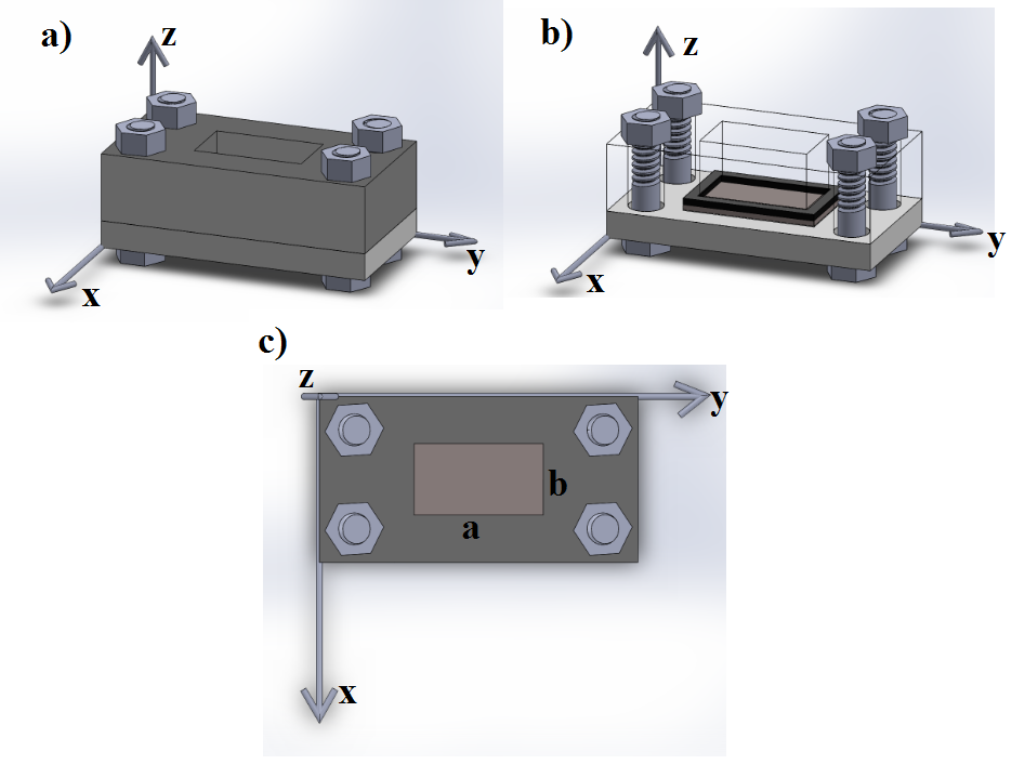
\includegraphics[scale=.2]{../Images/celdan2} 
	\caption{\emph{ Modelado mecánico en 3D, diseño de la celda Electroquimica donde podemos ver la forma de un prisma dando los datos requeridos y necesarios para los experimentos.  El diseño de la celda usada  es de $1.206\ \ cm^2$ (esta es la superficie atacada en el proceso), el área atacada es de forma rectangular ($0.62\ \ cm \times 2.03 \ \ cm$ ) y una altura ($1.2\ \ cm $) a) Celda completa b) Celda sin la tapa superior y c) Vista superior}}
	\label{fig:por1}
\end{figure}
Podemos ver en la Figura \textbf{\ref{fig:por1}} el modelado mecánico en 3D, diseño de la celda Electroquímica para tener una mejor optimización en la fabricación de silicio poros donde podemos ver la forma de un prisma dando los datos requeridos.  El diseño de la celda usada  es de $1.206\ \ cm^2$ (esta es la superficie atacada en el proceso), el área atacada es de forma rectangular ($0.62\ \ cm \times 2.03 \ \ cm$ ) y una altura ($1.2\ \ cm $), todo esto con fin de poder optimizar nuestros experimentos ajustado a todas las necesidades que esto requerían.
\begin{figure}[H]
	\centering
	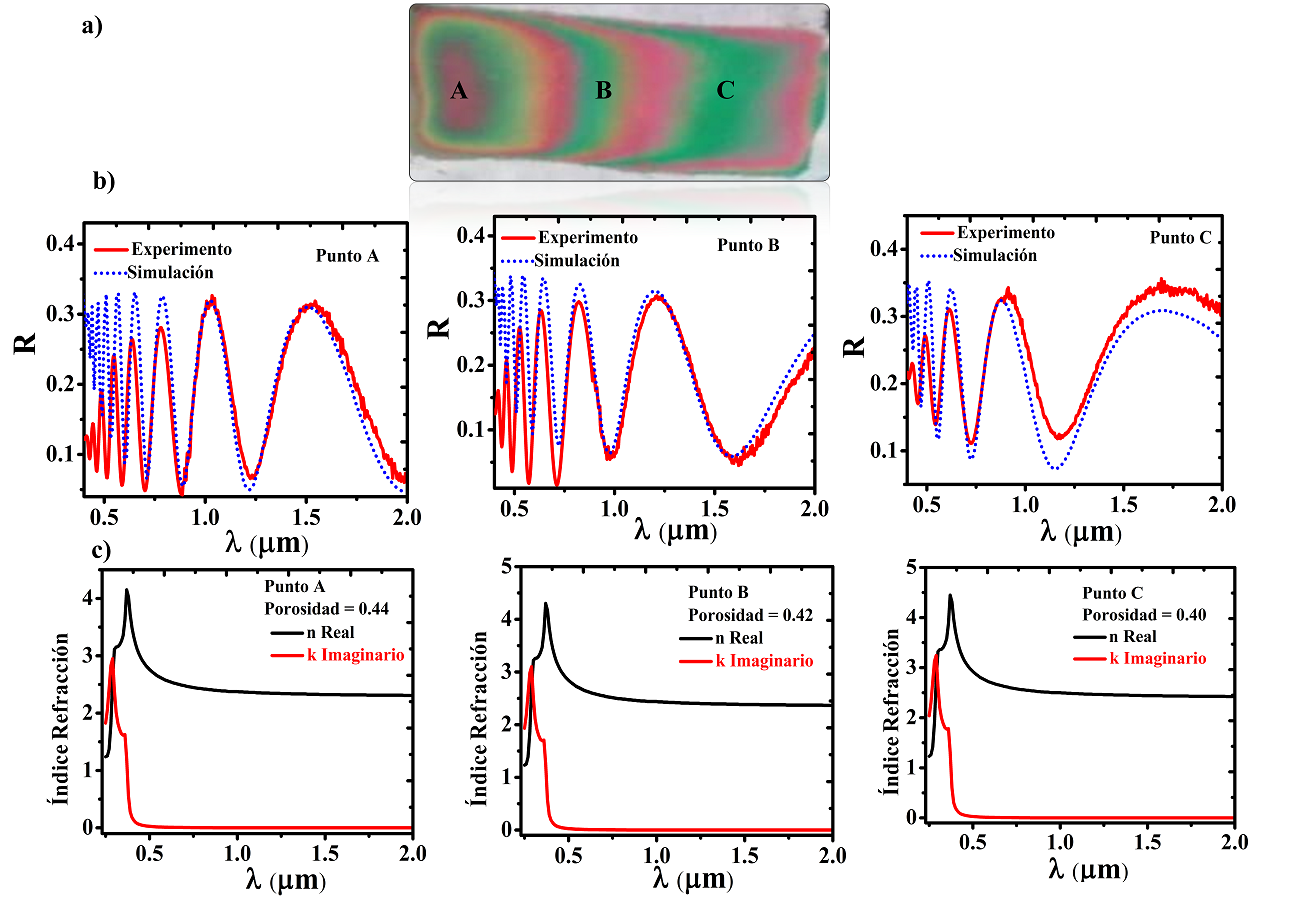
\includegraphics[scale=.35]{../Images/SPgrin51}
	\caption{\emph{a) Muestra de Silicio atacada  con una mezcla electrolítica de HF acuoso (concentración: 48 $ \% $ de peso), glicerol (pureza: 99.8$ \% $ de peso) y etanol (pureza: 99.9$ \% $ de peso) en 3:7:1 proporción de volumen, respectivamente. Obteniendo una  monopelicula de Silicio poroso con GRIN G1 con una corriente inicial  de G1(5 mA), con un tiempo de ataque de  600s.  Se consideran tres ubicaciones diferentes puntos denotado de la siguiente forma,  A(0.3cm) y  B(0.8 cm) y  C(1.7 cm). b) Las mediciones de la reflectancias para saber las propiedades ópticas en cada uno de los puntos y los ajustes que se produjo por medio de la ecuación \ref{Eq:ECMR}. c) Tenemos los indices de refracción del silicio poroso GRIN complejo, donde calculamos la parte real e imaginaria por medio de la ecuación \ref{Eq:Brugg}. para diferentes porosidades en cada punto, A(P=0.44), B(P=0.42) y C(P= 0.40) } }
	\label{fig:DR3}
\end{figure} 
La  Figura \textbf{\ref{fig:DR3} a)} se consideran tres ubicaciones en diferentes puntos denotado de la siguiente forma,  $A(0.3\ \ cm)$ y $ B(0.8 \ \  cm)$ y $ C(1.7 \ \  cm)$, de la  muestra de SiP GRIN $G1(I=5 mA)$. Así mismo las Fig. \textbf{\ref{fig:DR3} b)} , tenemos las mediciones de la reflectancias para saber las propiedades ópticas y los ajustes que se produjo por medio de la ecuación \textbf{\ref{Eq:ECMR}}. La Figura \textbf{\ref{fig:DR3} c) } son indices de refracción del silicio poroso GRIN complejo, donde calculamos la parte real e imaginaria por medio de la Ecuación \textbf{\ref{Eq:Brugg}}. para diferentes porosidades en cada punto, $A(P=0.44)$, $B(P=0.42)$ y $C(P= 0.40)$. La ubicación $A$ está mas cerca al electrodo, mientras que la ubicación de $C$ está más lejos al otro extremo de la muestra. Dado que la densidad de corriente se aplica desde un extremo, las lineas de campos atacan la muestra de forma lateral a la oblea de silicio, en la presente configuración, se hizo un montaje  basado en los datos simulados que se mostraron en la Fig.\textbf{ \ref{fig:DR1}}  la parte experimental se tomo un electrodo de platino tapando su superficie, dejando solo un área muy pequeña, como si fuese  una punta. La reacción electroquímico tiene lugar cuando le aplicamos corrientes desde un extremo ánodo(punta del electrodo) al sustrato de silicio (resistividad $0.002 - 0.005$ $ \Omega \cdot cm$), a través de un electrólito formando un circuito de corriente. Los espectros de reflectancia de las muestras recién grabada G1  medidas en los puntos $A(0.3\ \ cm)$ y $ B(0.8 \ \  cm)$ y $ C(1.7 \ \  cm)$ se presenta en la Fig. \textbf{\ref{fig:DR3} b)}, se les realizo un ajuste de reflectividad numérica usando el método de matriz de transferencia para el caso de una monopelicula porosa en Si.  Cabe destacar que el ajuste realizado, se consideró un rango espectral de la longitud de onda de los espectros de reflectividad experimentales para el cual el silicio se pueda considerar el indice complejo y de ese modo encontrar el  del índice de refracción del silicio poroso complejo con la finalidad de determinar la porosidad  y el espesor físico (nm) experimental por medio del SEM. La formación de SiP GRIN en el grosor  se produce debido a la variación en la concentración de los huecos disponible en la interfaz de electrólito de Si, por lo tanto, un aumento de la densidad de corriente  lateral aplicado aumenta la dimensión de los poros y su profundidad. De este modo, la extensión de la película porosa que muestra un gradiente que  se puede controlar desde la densidad  de corriente laterales.
\begin{figure}[H]
	\centering
	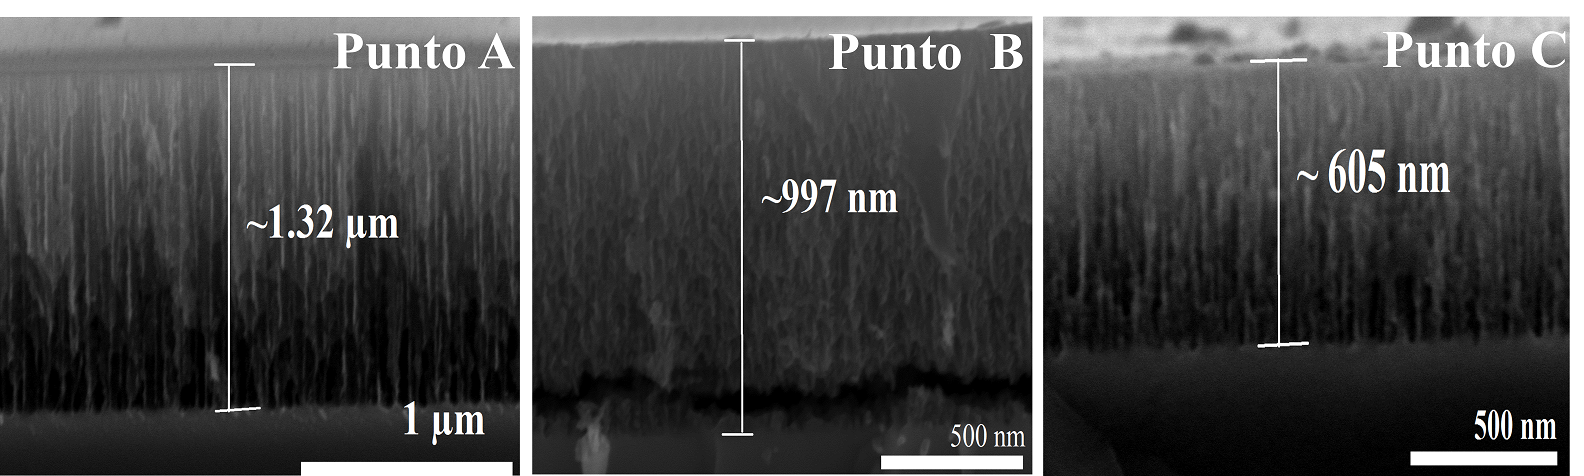
\includegraphics[scale=.3]{../Images/semD11}
	\caption{\emph{Caracterización de una monopelicula de SiP GRIN G1 con una corriente inicial  de  $5 \ \ mA$, viendo  la morfología y la profundidad de la sección trasversal de varias micrografias SEM , en diferentes puntos, $A(0.3\ \ cm)$ y $ B(0.8 \ \  cm)$ y $ C(1.7 \ \  cm)$. Vemos el tamaño de muestra para cada punto de medición, la profundidad  $d(A)=1320 \ \ nm$, $d(B)=997\ \  nm$ y $d(C)=605\ \  nm$ } }
	\label{fig:DR4}
\end{figure} 
La Figura \textbf{\ref{fig:DR4}} muestra las vistas en la sección trasversal en los puntos $A(0.3\ \ cm)$ y $ B(0.8 \ \  cm)$ y $ C(1.7 \ \  cm)$, podemos medir  los espesores para cada punto de la muestra $G1(I=5 \ \ mA)$, $d(A)=1320 \ \ nm$, $d(B)=997\ \  nm$ y $d(C)=605\ \  nm$. Así mismo, lo pudimos comprobar para una segunda  muestra $G2 (I=40 \ \ mA)$, con porosidades para cada puntos, $A(P=0.76)$, $B(P=0.73)$ y $C(P= 0.68)$ y las profundidades  $d(A)=1950 \ \ nm$, $d(B)=1690\ \  nm$ y $d(C)=1430\ \  nm$, diseñada de la misma forma que la muestra G1, solo variando la corriente teniendo en cuenta la relación de densidad de corriente para cada punto. Aparte de eso, se formó un gradiente estructural, a lo largo de la dirección $a$ del eje de las $x$, donde  punta del electrodo esta cerca del punto $A$ y alejado del  punto $C$ del sustrato, utilizando la configuración experimental propuesta. Además, se logró poder controlar la densidad de corriente en función de la posición de la muestra y la profundidad, vista en las micrografías SEM. 
\begin{figure}[H]
	\centering
	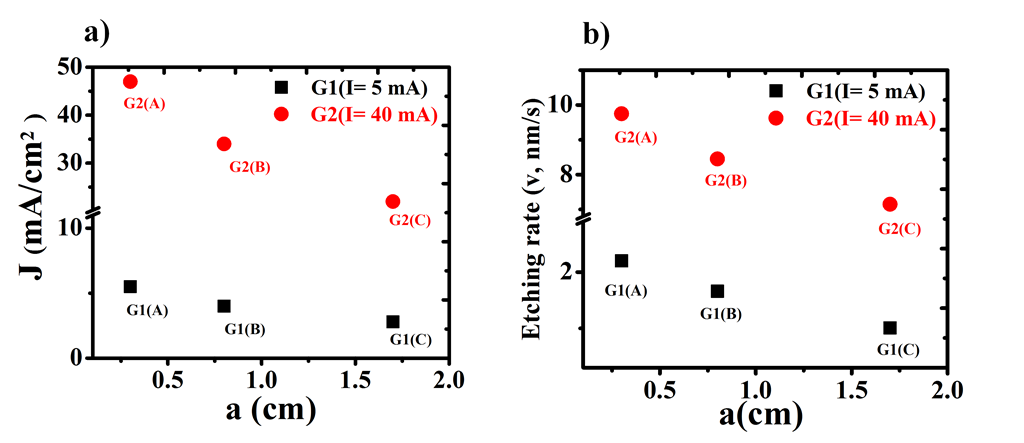
\includegraphics[scale=.45]{../Images/grinJDR}
	\caption{\emph{a) Relación  de la densidad de corriente $J(mA/cm^2) $ normalizado con la corriente eléctrica $I(mA)$, nos queda $J/I \sim 1.2 \ \ a \ \ 0.5 (1/cm^2) $, cuando se lo aplicamos a dos muestras $G1(I=5 \ \ mA)$ y $G2(I=40 \ \ mA)$  en función del eje $a$ $(0.1...2.0 \ \ cm)$, medidos en los puntos  $A(0.3\ \ cm)$ y $ B(0.8 \ \  cm)$ y $ C(1.7 \ \  cm)$. b) La velocidad de ataque $v=d(J_i)/t(nm/seg)$, las profundidades ( espesor $d(J_i)$, $i=$ $A(0.3\ \ cm)$ , $ B(0.8 \ \  cm)$ y $ C(1.7 \ \  cm) )$ sacada en micrografias del SEM $d(J_i)(nm)$ y los tiempos de ataques $G1(t=600 \ \ seg)$ y $G2(t=200 \ \ seg)$, en función del eje $a$ $(0.1...2.0 \ \ cm)$  } }
	\label{fig:JDR}
\end{figure}
En la Figura \textbf{\ref{fig:JDR} a)}  Relación  de la densidad de corriente $J(mA/cm^2) $ normalizado con la corriente eléctrica $I(mA)$, nos queda $J/I \sim 1.2 \ \ a \ \ 0.5 (1/cm^2) $, cuando se lo aplicamos a dos muestras $G1(I=5 \ \ mA)$ y $G2(I=40 \ \ mA)$  en función del eje $a$ $(0.1...2.0 \ \ cm)$, medidos en los puntos  $A(0.3\ \ cm)$ y $ B(0.8 \ \  cm)$ y $ C(1.7 \ \  cm)$. 
La  Fig. \textbf{\ref{fig:JDR} b)} podemos calcular la velocidad de ataque $v=d(J_i)/t(nm/s)$, donde las profundidades ( espesor $d(J_i)$, $i=$ $A(0.3\ \ cm)$ , $ B(0.8 \ \  cm)$ y $ C(1.7 \ \  cm) )$ sacada en micrografias del SEM $d(J_i)(nm)$ y los tiempos de ataques $G1(t=600 \ \ s)$ y $G2(t=200 \ \ s)$, en función del eje $a$ $(0.1...2.0 \ \ cm)$. 
\begin{figure}[H]
	\centering
	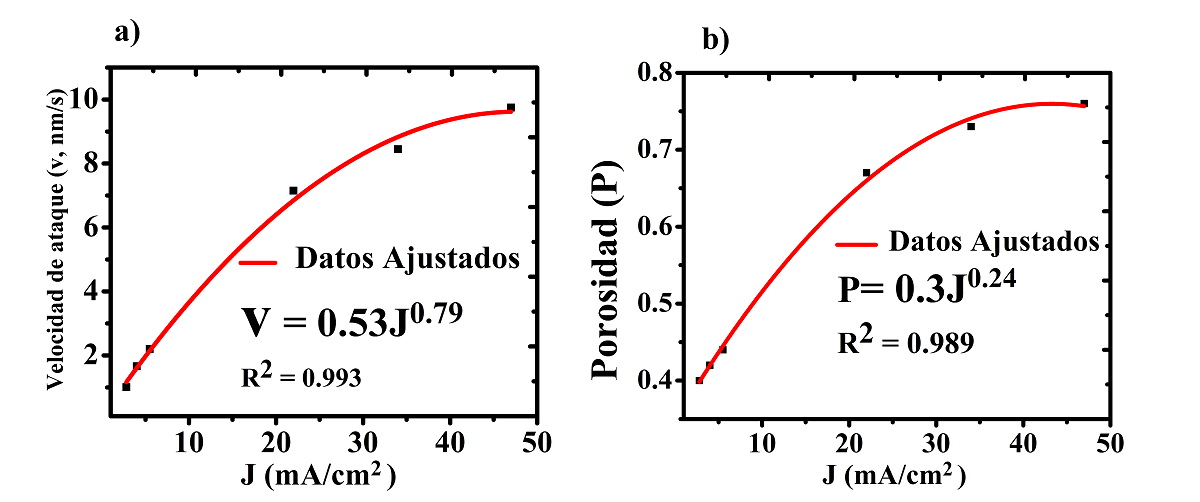
\includegraphics[scale=.4]{../Images/grinJD31}
	\caption{\emph{ Se obtuvieron las relaciones de las muestras las muestras $G1 (I=5 mA)$ y $G2 (I=40 mA)$ para hallar: a) Velocidad de ataque con la densidad de corriente para cada punto y b) Porosidad en función de  la densidad de corriente. Con esto tenemos las curvas de calibración para la fabricación de cualquier estructura de silicio poroso GRIN    } }
	\label{fig:Indr1}
\end{figure}
La Figura\textbf{ \ref{fig:Indr1} a)} se explica detalladamente las relaciones que salen al diseñar las muestras $G1 (I=5 mA)$ y $G2 (I=40 mA)$. Para el primer caso $G1$  las profundidades ($1320 \ \ nm$ a $605\ \ nm$) y las densidades de corrientes ($6 \ \ mA/cm^2$ a $2.5 \ \ mA/cm^2$), encontrando la velocidad de ataque $2.2 \ \ nm/s$ hasta $1.1 \ \ nm/s$ relacionada con profundidad y el tiempo ($600 \ \ s$ ) de exposición de la muestra, con la densidad de corriente. También  encontramos la profundidad  ($1950 \ \ nm$ a $1430 \ \ nm$) y la densidad   de corriente ($50 \ \ mA/cm^2$ a $20 \ \ mA/cm^2$) en función de los puntos de medición de la muestra  $G2 (I=40 mA)$. Pudimos obtener  la velocidad de ataque de $9.8\ \ nm/s$ hasta $7.1 \ \ m/s$ relacionando con la profundidad  y el tiempo ($200 \ \ s$), con la densidad de corriente. Una vez conocida el espesor de la monopelicula y el tiempo de ataque aplicado a las mismas, se calculó la velocidad de ataque  de acuerdo con la formula $v=d/t$, para cada una de las   densidades de corrientes en los puntos  $A(0.3\ \ cm)$ y $ B(0.8 \ \  cm)$ y $ C(1.7 \ \  cm)$. Luego ajustamos una función a los puntos de la velocidad de ataque con las diferentes densidades de corrientes permitidas por la condición de anodización.  Para un espesor $d(J_i)$ deseado, se calcula el tiempo de ataque $t$ (así que, $t=v/d(J_i)$) y podemos diseñar cualquier estructura conociendo la densidad de corriente y el tiempo de ataque.
Así mismo, la Figura \textbf{\ref{fig:Indr1}} b) encontramos una relación de la porosidad para cada posición con su determinada densidad de corriente. Por lo tanto, si se desea fabricar una monopeliculas de SiP de cierta porosidad con un determinado espesor, basta con recurrir a las gráficas de la Figura \textbf{\ref{fig:Indr1}}  para determinar la densidad de corriente que le corresponde, velocidad de ataque y consecuentemente el tiempo, obteniendo para esa monopeliculas. La importancia de las curvas de calibración radica en que nos permite tener una relación de las porosidades que se pueden alcanzar (y por consecuencia tener control sobre los índices de refracción posibles) en función de la densidad de corriente y ser capaces de controlar los espesores de las capas que se fabricarían, al controlar la el tiempo de ataque para cada una de las corrientes elegidas.


\subsection{Microcavidades de Silicio Poroso GRIN}
\begin{figure}[H]
	\centering
	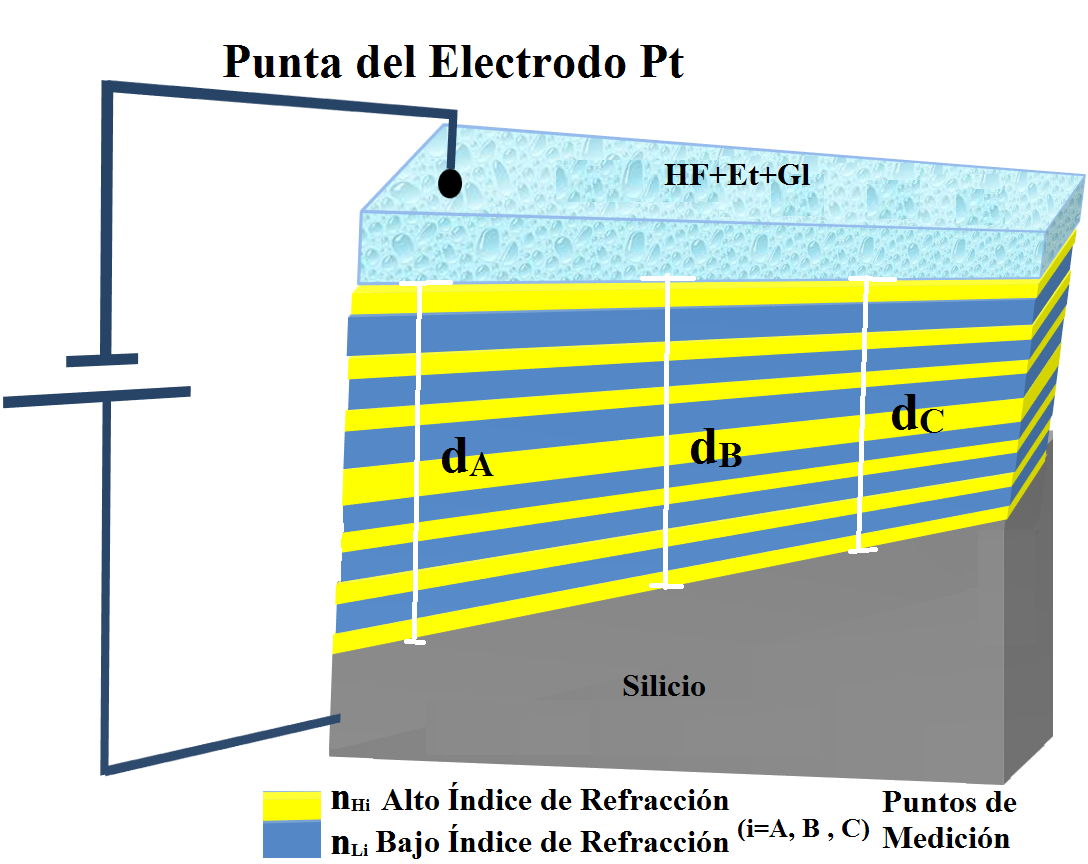
\includegraphics[scale=0.2]{../Images/MicrGrin}
	\caption{\emph{ Esquema de una Microcavidad de Silicio Poroso GRIN.  Se obtienen capas alternas de alto $(H)$ índice de refracción $n_{_{Hi}}$ y bajo $(L)$ índice de refracción  $n_{_{Li}}$, donde $N_{_{H}}$ es el numero de capas para  $n_{_{Hi}}$ y $N_{_{L}}$ es el numero de capas para  $n_{_{Li}}$. Entonces, $d_{_{Hi}}$ es el espesor de la monopelicula de  $n_{_{Hi}}$ en ese punto de medición y $d_{_{Li}}$ es el espesor de la monopelicula de  $n_{_{Hi}}$ en ese punto de medición. Por lo que, $d_{_{i}}$ es el espesor total calculado para cada una de la mediciones, definiendo a $i=$ A, B, C. Teniendo la siguiente relación $d_{_{i}} = (N_{_{Hi}}d_{_{Hi}})+(N_{_{Li}}d_{_{Li}}) + (2d_{_{Hi}})$. }}
	\label{fig:MCGRIN0}
\end{figure}
La Figura\textbf{ \ref{fig:MCGRIN0}}. se muestra el esquema de como debe ser un gradiente lateral propuesto inicialmente para monopeliculas en la sección 4.2, donde diseñamos una celda electolitica adecuada para nuestros experimentos y dándonos los resultados esperado de la simulación de la sección 4.1. Ahora nuestro propósito es fabricar estructuras fotonicas mas complejas como son las Microcavidades  de Silicio Poroso GRIN, teniendo en cuenta que partimos de tener un electrodo de punta casi sobre la superficie y haciendo una variacion de corrientes podemos conseguir el efecto de alternar las capas.  Se obtienen capas alternas de alto $(H)$ índice de refracción $n_{_{Hi}}$ y bajo $(L)$ índice de refracción  $n_{_{Li}}$, donde $N_{_{H}}$ es el numero de capas para  $n_{_{Hi}}$ y $N_{_{L}}$ es el numero de capas para  $n_{_{Li}}$. Entonces, $d_{_{Hi}}$ es el espesor de la monopelicula de  $n_{_{Hi}}$ en ese punto de medición y $d_{_{Li}}$ es el espesor de la monopelicula de  $n_{_{Hi}}$ en ese punto de medición. Por lo que, $d_{_{i}}$ es el espesor total calculado para cada una de la mediciones, definiendo a $i=$ A, B, C. Teniendo la siguiente relación $d_{_{i}} = (N_{_{Hi}}d_{_{Hi}})+(N_{_{Li}}d_{_{Li}}) + (2d_{_{Hi}})$.
Los datos iniciales para diseño convencional utilizamos $\lambda_{_{c}}= 0.67 \ \ \mu m$, $n_{_{H}} =2.6$, $P_{_{H}} =0.46$, $d_{_{H}}=0.066 \ \ \mu m  $, $t_{_{H}}=35 s  $ y para  $n_{_{L}}= 1.4$,  $P_{_{L}} =0.75$, $d_{_{L}}=0.117 \ \ \mu m  $, $t_{_{L}}=11 s  $. Todos estos datos son para el punto $0$  que esta ubicado a un extremo de la muestra justamente debajo del contra-electrodo de punta. 
\begin{figure}[H]
	\centering
	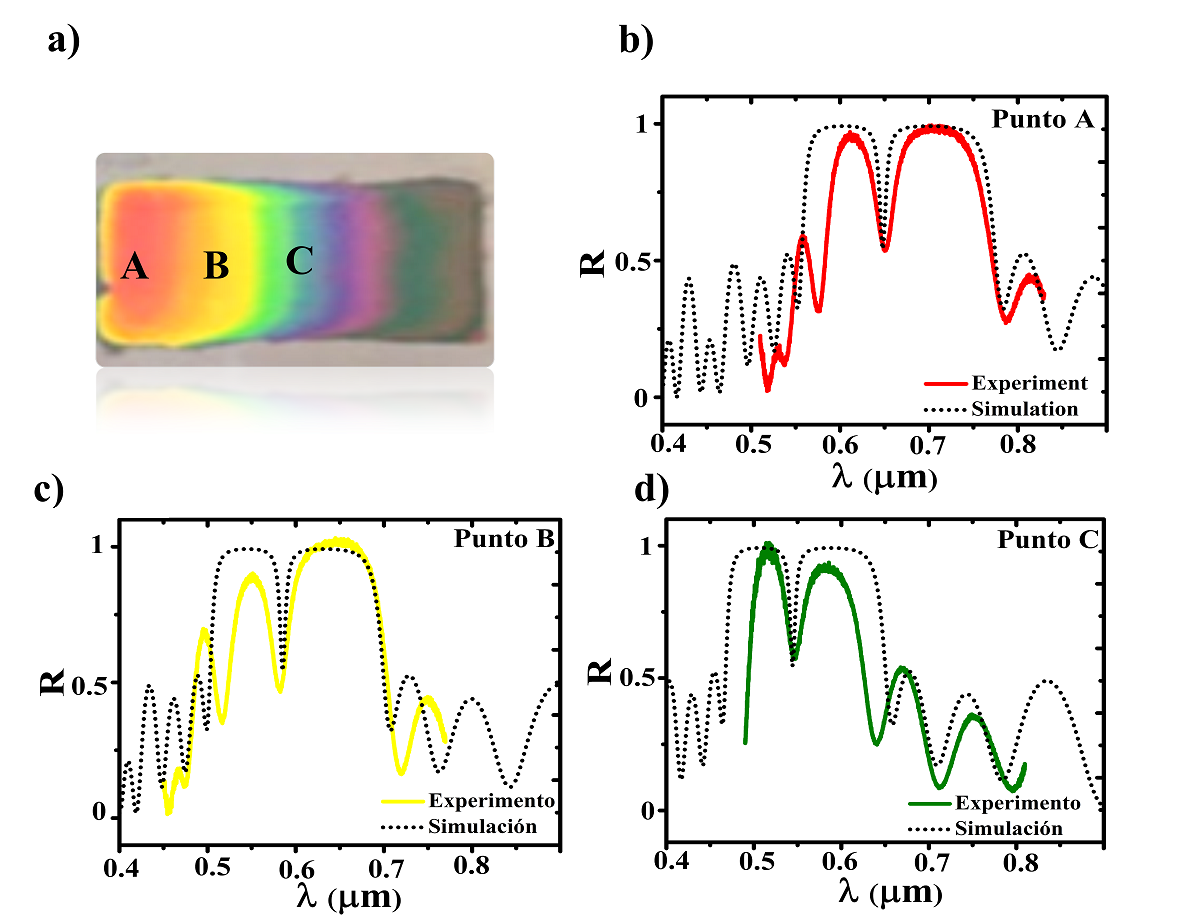
\includegraphics[scale=.4]{../Images/MCGRIN211}
	\caption{\emph{a) Se consideran tres ubicaciones en diferentes puntos denotado de la siguiente forma,  $A(0.3\ \ cm)$ y $ B(0.8 \ \  cm)$ y $ C(1.2 \ \  cm)$, de la  muestra de SPMCGRIN $GMC$.  b) Tenemos las mediciones de la reflectancias para saber las propiedades ópticas con la simulación propuesta. Pudimos mostrar que en una estructura de Silicio Poroso GRIN, para una microcavidad los datos esta muy acorde la simulación y el experimento, encontramos los indices de refracción y las porosidades en función de la densidad de corriente en cada punto de medición, ver tabla \ref{tabla:1}. }}
	\label{fig:MCGRIN3}
\end{figure}
\begin{table}[H]
	\centering
	\begin{tabular}{|c|c|c|c|c|c|c|}
		\hline 
		\textbf{Puntos} & $\lambda_c (\mu m)$ & \textbf{n} & \textbf{k} & \textbf{Porosidad} & \textbf{J}$(mA/cm^2)$ & \textbf{t(s)}\\ 
		\hline 
		A(H) & 0.65 & 2.661 & 0.0264 & 0.45 & 5.5 & 35 \\ 
		\hline 
		B(H) & 0.58 & 2.762 & 0.0135 & 0.41 & 4.0 & 35 \\ 
		\hline 
		C(H) & 0.54 & 2.808 & 0.0178 & 0.39 & 3.0 & 35 \\ 
		\hline 
		A(L) & 0.65 & 1.442 & 0.0015 & 0.74 & 44 & 11 \\ 
		\hline 
		B(L) & 0.58 & 2.295 & 0.0091 & 0.68 & 32 & 11 \\ 
		\hline 
		C(L) & 0.54 & 2.302 & 0.001 & 0.64 & 24 & 11 \\ 
		\hline 
	\end{tabular} 
	\caption{ \emph{Tenemos  diferentes puntos denotado de la siguiente forma,  $A(0.3\ \ cm)$ y $ B(0.8 \ \  cm)$ y $ C(1.2 \ \  cm)$, de la  muestra de una Microcavidad de Silicio Poroso GRIN (SiPMCGRIN) $GMC$. Se obtienen capas alternas de alto índice de refracción (H) y bajo índice de refracción (L) en cada uno de los puntos de medición (A,B y C). Los índice de refracción de las SiPMCGRIN se consideraron de los valores experimentales y teóricos que se obtuvieron para la porosidad ($P=0.3J^{0.24}$). Y el tiempo de ataque lo pudimos obtener con la relación de $V=0.53J^{0.79}$ donde $t=d/V$.}}
	\label{tabla:1}
\end{table}

En la  Figura \ref{fig:MCGRIN3}. a) se consideran tres ubicaciones en diferentes puntos denotado de la siguiente forma,  $A(0.3\ \ cm)$ y $ B(0.8 \ \  cm)$ y $ C(1.2 \ \  cm)$, de la  muestra de SiPMCGRIN $GMC$. Así mismo, la Figura \ref{fig:DR3}. b) , tenemos las mediciones de la reflectancias para saber las propiedades ópticas con la simulación propuesta . Podemos ver como a partir de un arreglo experimental tenemos algunos resultados importante producto de toda una curva de calibración adecuada para fabricar silicio poroso GRIN.  Los índice de refracción de las Microcavidades  de Silicio Poroso GRIN se consideraron los valores experimentales y teóricos que se obtuvieron para la porosidad y los espesores que se muestran en la Tabla 1.  Las microcavidades de silicio poroso (MCSiP) con índice de refracción con gradiente (GRIN), fueron fabricadas con diferentes densidades de corrientes variaba de $6 \ \ mA/cm^2$ a $2.5 \ \ mA/cm^2$ para una corriente de $5 \ \  mA$, para un  $t_{_{H}}=35 s  $, con alto índice de refracción $n_{_{H}} \sim$  $2.661$ a $2.808$  y  porosidades de $P_{_{H}} \sim$ $0.45$ a $0.39$. También para  $44\ \ mA/cm^2$ a $24\ \  mA/cm^2$, corriente de $38 \ \  mA$, utilizando $t_{_{H}}=11 s$ para bajo índice de refracción $n_{_{L}}\sim$  $1.448$ a $2.267$ y con porosidades de $P_{_{L}} \sim$ $  0.75 $ a $ 0.64 $. La porosidad se calculo con la curva de calibración expuesta en la   ($P=0.3J^{0.24}$). Y el tiempo de ataque lo pudimos obtener con la relación de $V=0.53J^{0.79}$ donde $t=d/V$  y los índice de refracción utilizando la fórmula de Bruggeman. Para los valores teóricos, utilizamos los índices de refracción complejos como parámetros libres para ajustar los espectros de reflactancia experimentales (Sección 4.2). 
\begin{figure}[H]
	\centering
	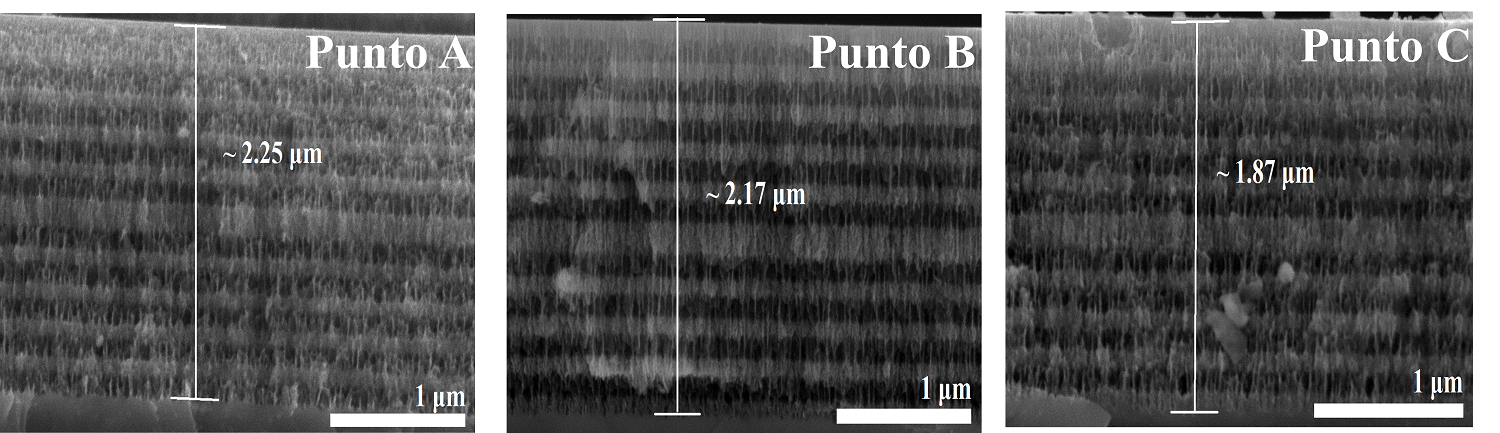
\includegraphics[scale=.3]{../Images/MCGRINSEM}
	\caption{\emph{Imagen SEM del perfil de la sección transversal de las microcavidades con GRIN.}}
	\label{fig:MCGRIN4}
\end{figure}
La Figura \ref{fig:MCGRIN4}. muestra las imágenes transversales de SEM de las muestras de SiP empleadas en este trabajo. Rugosidad de la interfaz relativamente pequeña y un claro contraste entre el alto y bajo porosidad  de la microcavidad medida en diferentes putos (A, B y C), mostrando el cambio de espesores en cada una de estas. 
Los espesores medidos de las estructuras multipeliculas completas mostraron una buena concordancia con las  simulaciones tomado de $V=0.53J^{0.79}$ donde $d_j=Vt_j$ ($j=H,L$), que son los espesores de cada una de la monopelicula de la microcavidad de silicio poroso GRIN en los puntos de medición y el espesor total  lo encontramos como  $d_{_{i}} = (N_{_{Hi}}d_{_{Hi}})+(N_{_{Li}}d_{_{Li}}) + (2d_{_{Hi}})$  definiendo a $i=$ A, B, C. Lo que resultó en (medido / simulación) $2.25 / 2.31 \ \ \mu m $ (para estructura en Punto A), $2.17 / 2.08 \ \ \mu m $ (para estructura en el punto B) y $1.87 / 1.65 \ \ \mu m $ (para estructura  en el punto C). Pudiendo decir que para cada puntos de mediciones le corresponde diferentes densidades de corrientes calculada, lo que corresponden a diferentes espesores al final de la fabricación viendo claramente el gradiente lateral producto de nuestro experimento.
\section{Conclusión}
Se derivaron las expresiones necesarias para las componentes del potencial, encontrándonos una relación de la punta del contraelectrodo que actúa análogamente como una carga puntual y la densidad de corriente para una geometría en una caja electrolítica rectangular y resolvemos las ecuaciones electrostática con condiciones de contornos adecuadas. Dando como resultado un modelo electrostático para cristales con índice de refracción con gradiente (MECFGRIN).
Es la primera vez que el formalismo aquí mencionado se aplica para encontrar la densidad de corriente para diseñar silicio poroso. La forma del electrodo, el Área de la celda  produce una visible disminución en el tamaño y densidad de los poros. Adicionalmente,  optimizando las propiedades estructurales para una solo estructura pudimos tener un gradiente con diferentes profundidades, reflactancias en diferentes  punto de medición. De ese modo, pudimos simular la relación directa de la velocidad de ataque con la densidad de corrientes en los punto de la muestras de interés. A la vez desarrollamos una caracterización entre porosidad, índices de refracción del silicio poroso, con las diferentes densidades de corrientes.


\chapter{Aplicación: Sensado de etanol evaporado usando cristales fotónicos con indices de refracción con gradiente (GRIN)}
\label{Mo:SENSADO}
\markboth{CAPÍTULO 6. Aplicación: Sensado de etanol...}{}
\section{Introducción}
La detección de especies químicas y biológicas mediante la transducción óptica en estructuras SiP se investigó exhaustivamente durante los últimos veinticinco años desde los primeros informes del grupo de Sailor sobre el cambio de las propiedades ópticas de la monocapa de SiP tras la exposición a varios vapores orgánicos \cite{ssn1, ssn2}. Posteriormente, se ha informado sobre la detección de compuestos orgánicos volátiles (COV), gases inorgánicos, explosivos, organofosfatos, ADN, proteínas y otras biomoléculas en medio acuoso. Varias revisiones recientes describieron el progreso y los desafíos en el campo de los sensores químicos y biológicos SiP \cite{ssn3, ssn4, ssn5}. Todos cubren toda el área de detección de SiP (químico, bio, vapores, líquidos, lecturas eléctricas y ópticas) sin una selección específica de métodos de transducción y una fase de moléculas de analito (líquido / vapor). Por lo tanto, creemos que esta breve revisión, centrada únicamente en los métodos ópticos para la detección de vapores, será
relevante para la sistematización de diferentes enfoques de detección y estructuras SiP apropiadas. Los biosensores ópticos SiP y quimiosensores en un medio líquido (por ejemplo, iones metálicos, toxinas disueltas en agua) y dispositivos eléctricos SiP (excepto la detección multiparamétrica que involucra señales ópticas) están fuera del alcance de esta revisión. Durante las últimas décadas, la detección de gases ha atraído una gran atención en el mundo académico y la industria debido a sus aplicaciones generalizadas en monitoreo ambiental, seguridad nacional,
control de emisiones industriales, diagnósticos de aliento no invasivos y control de calidad de los alimentos \cite{ssn6}. Los sensores de gas óptico tienen un avance crítico sobre los detectores de gas que emplean lectura eléctrica (resistiva, capacitiva, onda gravimétrica de superficie acústica, etc.)): la falta de necesidad de contactos metálicos y acoplamiento de cables. Se pueden implementar en lugares
inaccesibles y en entornos hostiles mediante la interrogación de separación seguida por el procesamiento de la señal. Sin embargo, al igual que otros dispositivos de detección, los detectores de gas óptico se enfrentan a varios desafíos clave, que incluyen: sensibilidad, especificidad,
discriminación de interferencias, tiempo de respuesta y recuperación, deriva de fondo y envejecimiento. Afortunadamente, para el Si poroso, algunos de los desafíos anteriores se pueden resolver debido a la increíble diversidad de estructuras SiP, morfología del material, química de la
superficie y mecanismos de transducción óptica. La Figura 1 muestra los componentes principales de los sensores de gas óptico SiP que se pueden sistematizar en tres grandes grupos: estructura SiP, composición SiP y métodos de transducción óptica.
\begin{figure}[H]
	\centering
	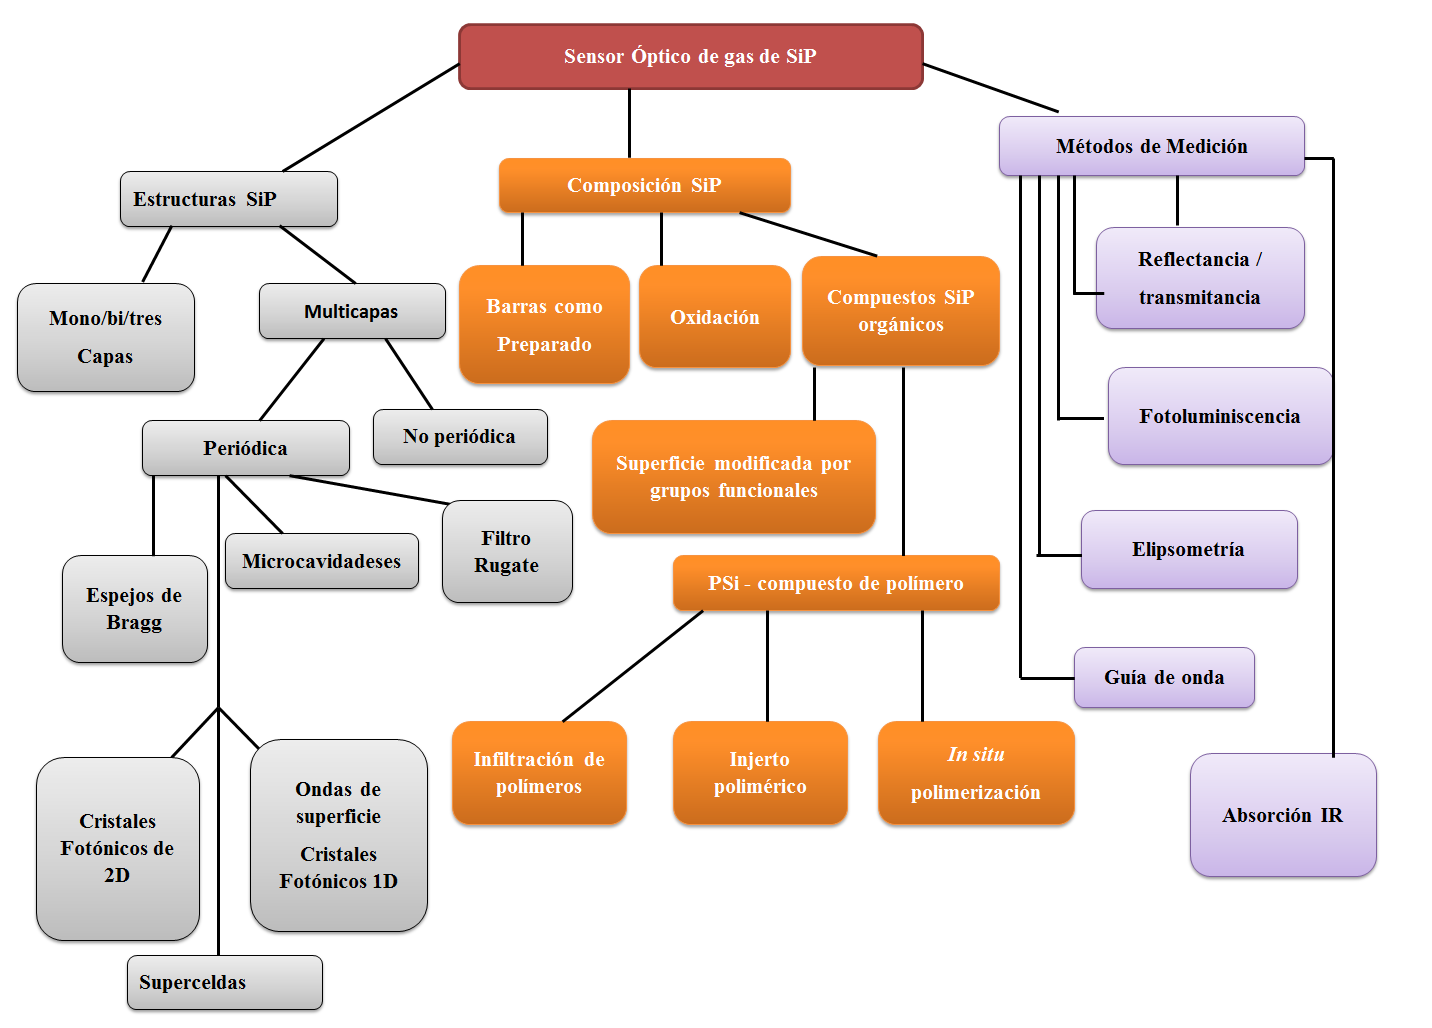
\includegraphics[scale=.3]{../Images/SemSip}
	\caption{\emph{ Un diagrama que  muestra los componentes principales de	los sensores de gas óptico SiP que se pueden sistematizar en tres grandes grupos: estructura SiP, composición SiP y métodos de transducción óptica\cite{GAU}. } }
	\label{fig:SemSip1}
\end{figure}

Hay una vasta y creciente cantidad de estudios en esta área, cuyo objetivo es mejorar el rendimiento de los sensores a través de una sofisticada funcionalización de la superficie, arquitecturas novedosas, lectura multiparamétrica y plataforma de matriz de sensores, junto con algoritmos de reconocimiento de patrones y procesamiento inteligente de señales. Esta revisión se centra principalmente en los avances recientes en el campo de los detectores ópticos de gas SiP para sistematizar y resaltar las tendencias y estrategias más prometedoras hacia la mejora del sistema para aplicaciones de detección de gases\cite{GAU}. Después de una breve descripción de los primeros trabajos relacionados con los mecanismos de transducción óptica y las estructuras basadas en SiP, se presentarán y discutirán los temas clave de la investigación actual y futura.
%%%%%%%%%%%%%%%%%%%%%%%%%%%%%%%%%%%%%%%%%%%%%%%%%%%%%%%%%%%%%%%%%%%%%
\section{Detalles Experimentales}
\subsection{Análisis de espectrometría infrarroja de transformada de Fourier (FTIR)}
Los espectros FTIR infrarrojos de transmisión se registraron utilizando un espectrómetro Nicolet MAGNA-IR 860 a una resolución de 2 cm-  . Las muestras se montaron en una cámara de muestra purgada. Los espectros de fondo se obtuvieron
utilizando una oblea de Si (100) plana sin tratar.

\subsection{Fabricación Sensor  en silicio poroso GRIN}
\begin{figure}[H]
	\centering
	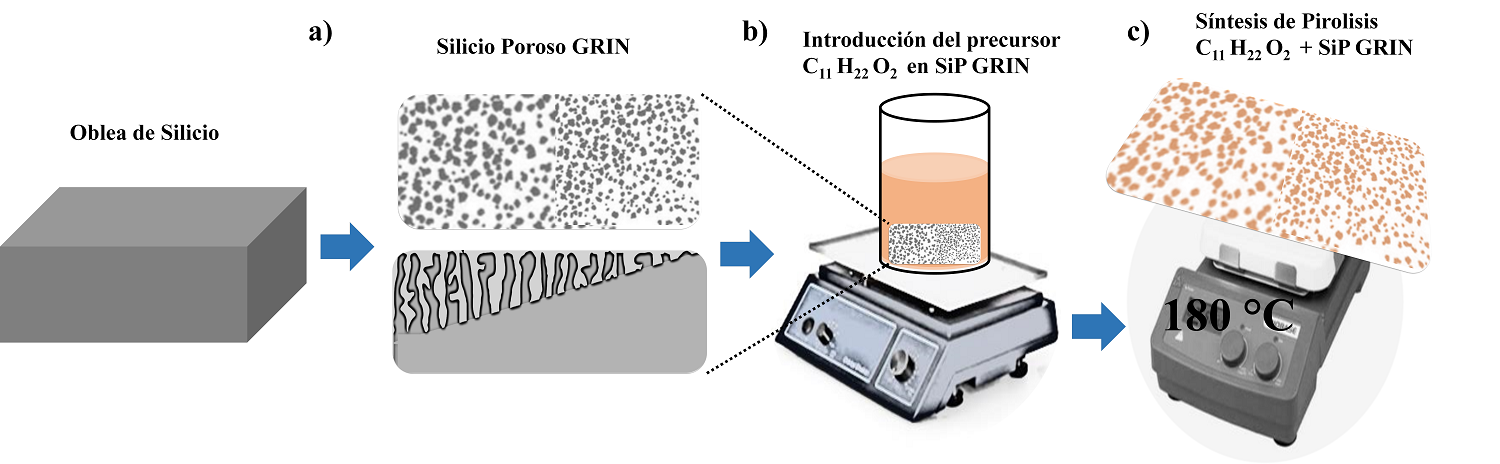
\includegraphics[scale=.3]{../Images/Esquema} 
	\caption{\emph{El diagrama esquemático del proceso de síntesis de pirólisis con ácido undeconoico (AU) en silicio poroso GRIN.  a ) El grabado químico electroquímico anódico se utiliza para preparar una capa de SiP a partir de una oblea de Si de cristal único.  b ) Introducción del precursor $C_{_{11}}H_{_{22}}O_{_{2}}$ en silicio poroso GRIN sobre un agitador. c ) el precursor se incorpora en los poros de SiP GRIN para la síntesis de pirólisis a $180C$.  }}
	\label{fig:REc0}
\end{figure}
La figura \textbf{\ref{fig:REc0}} es el diagrama esquemático del proceso de síntesis de pirólisis con ácido undeconoico (AU), (también llamado ácido undecílico) es un ácido carboxílico de origen natural, filtrado en silicio poroso GRIN. Apariencia, Sólido cristalino blanco/incoloro, Densidad:890 kg/$m^3$; 0,89 g/$cm^3$, Masa molar: 186,29 g/mol \cite{UA3, UA4}. La Fig. \textbf{\ref{fig:REc0} a)}  a) El grabado químico electroquímico anódico se utiliza para preparar una capa de SiP a partir de una oblea de Si de cristal único.  En la Fig. \textbf{\ref{fig:REc0} b)} Introducción del precursor $C_{_{11}}H_{_{22}}O_{_{2}}$  en silicio poroso GRIN sobre un agitador. Y para la Figura  Fig. \textbf{\ref{fig:REc0} c) } el precursor se incorpora en los poros de SiP GRIN para la síntesis de pirólisis a $180C$. Cabe señalar que los detalles experimentales para cualquier estructura de silicio poroso con GRIN esta explicado en el Capítulo \ref{Mo:MODELOGRIN} 
\section{Discusión y Resultados}

\subsection{ Sensor de  silicio poroso}
La disponibilidad de varias moléculas con diferentes grupos funcionales compatibles con enlaces de silicio-hidrógeno permitirá la fácil inmovilización de diferentes especies químicas y biológicas en el sustrato de SiP de área de superficie alta. Este paso abrirá nuevas oportunidades en el creciente campo de los biosensores.
\begin{figure}[H]
	\centering
	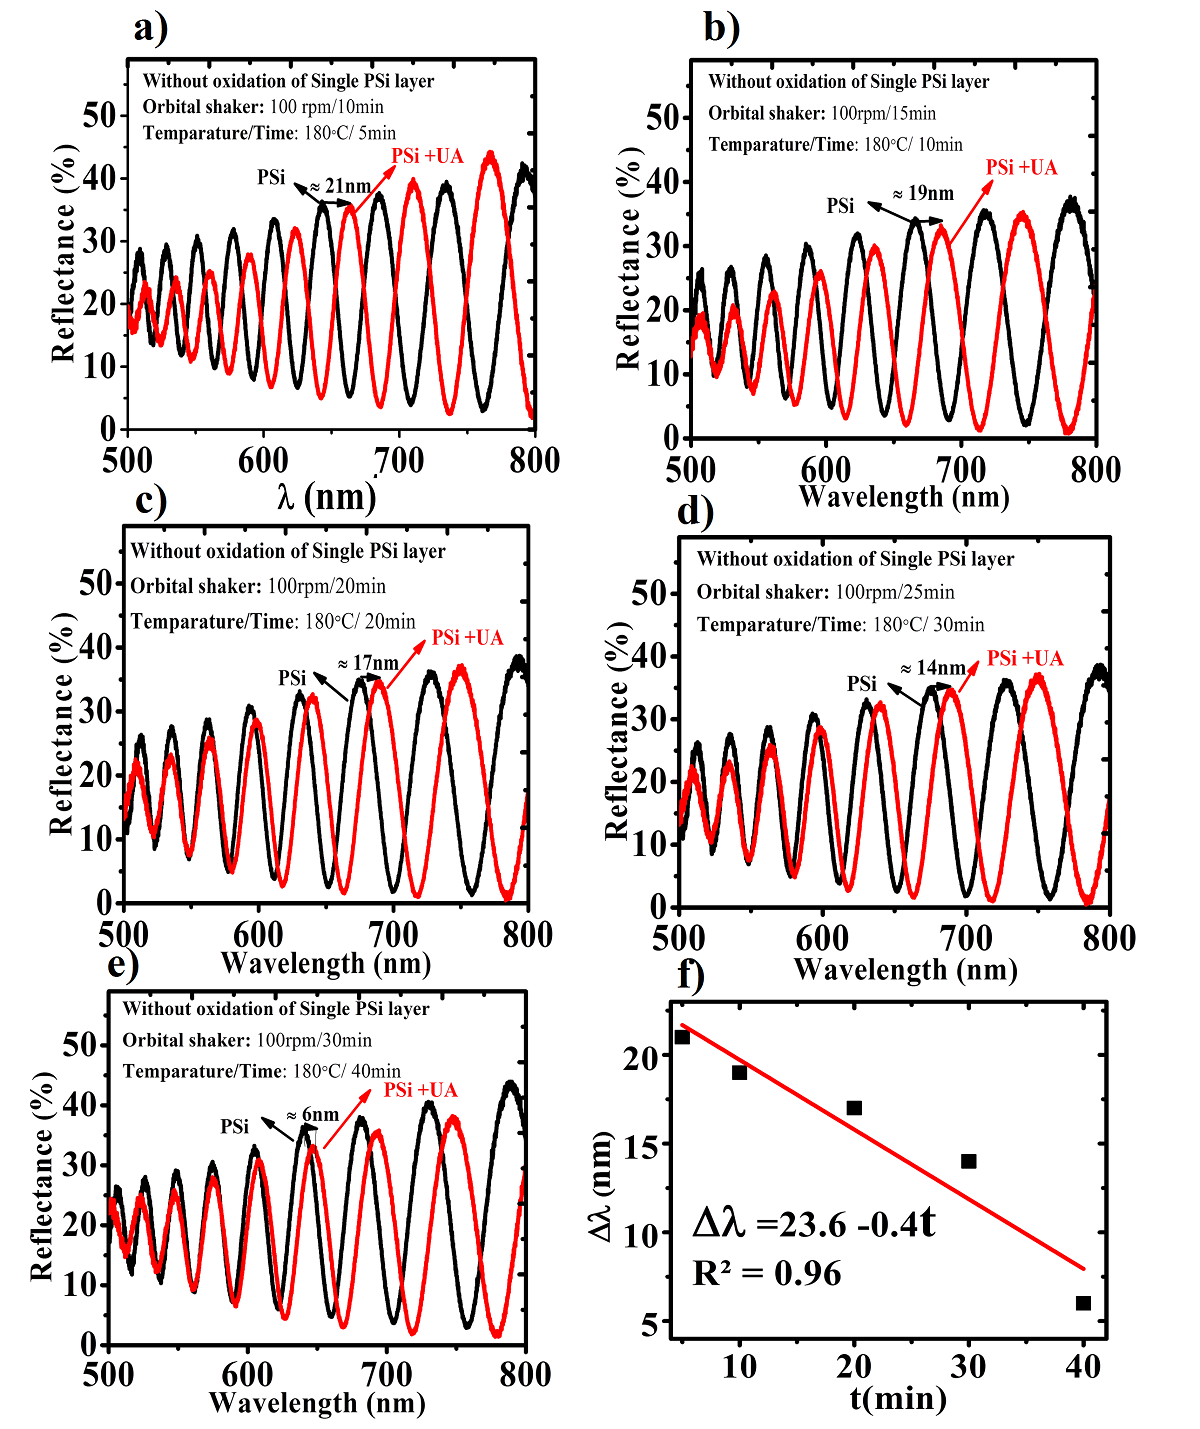
\includegraphics[scale=.3]{../Images/sens1}
	\caption{\emph{Espectro de reflectancias ($\%$) en función de la longitud de onda (nm). a) El espectro de reflectancia de color negro es silicio poroso y  el de colo rojo es cuando la funcionalizamos por medio de síntesis de pirólisis con ácido undeconoico (AU) , agitándolo a 100 rpm con un tiempo de 10 min con una temperatura de 180 C por 5 min. b) El color negro SiP y rojo SiP+AU agitándolo a 100 rpm con un tiempo de 15 min con una temperatura de 180 C por 10 min. c) El color negro SiP y rojo SiP+AU agitándolo a 100 rpm con un tiempo de 20 min con una temperatura de 180 C por 20 min. d) El color negro SiP y rojo SiP+AU agitándolo a 100 rpm con un tiempo de 25 min con una temperatura de 180 C por 30 min. e) El color negro SiP y rojo SiP+AU agitándolo a 100 rpm con un tiempo de 30 min con una temperatura de 180 C por 40 min. f) Encontramos una relación de la diferencias de espectros de reflactancia de SiP y cuando SiP+AU  en función del tiempo $ \Delta \lambda =23.6 -0.4t$} }
	\label{fig:REc1}
\end{figure}
En la figura \textbf{\ref{fig:REc1}} Espectro de reflectancias ($\%$) en función de la longitud de onda (nm). La figura \textbf{\ref{fig:REc1} a)} El espectro de reflectancia de color negro es silicio poroso y  el de colo rojo es cuando la funcionalizamos por medio de síntesis de pirólisis con ácido undeconoico (AU) , agitándolo a 100 rpm con un tiempo de 10 min y luego expuesto a una temperatura de 180 C por 5 min, siendo $\Delta \lambda \approx 21 nm$. La figura \textbf{\ref{fig:REc1} b)} El color negro SiP y rojo SiP+AU agitándolo a 100 rpm con un tiempo de 15 min y lo pasaron a una temperatura de 180 C por 10 min, tenemos que  $\Delta \lambda \approx 19 nm$. En la figura \textbf{\ref{fig:REc1}c)} el color negro SiP y rojo SiP+AU agitándolo a 100 rpm con un tiempo de 20 min y lo pasaron a una  temperatura de 180 C por 20 min, siendo $\Delta \lambda \approx 17 nm$.  La figura \textbf{\ref{fig:REc1} d)} el color negro SiP y rojo SiP+AU agitándolo a 100 rpm con un tiempo de 25 min y lo colocaron  a una temperatura de 180 C por 30 min y encontramos $\Delta \lambda \approx 14 nm$. Para la figura \textbf{\ref{fig:REc1} e)} El color negro SiP y rojo SiP+AU agitándolo a 100 rpm con un tiempo de 30 min y expuesto a una temperatura de 180 C por 40 min y  $\Delta \lambda \approx 6 nm$. Y por ultimo,  la  figura \textbf{\ref{fig:REc1} f)} encontramos una relación de la diferencias de espectros de reflactancia de SiP con SiP+AU  en función del tiempo $ \Delta \lambda =23.6 -0.4t$
\begin{figure}[H]
	\centering
	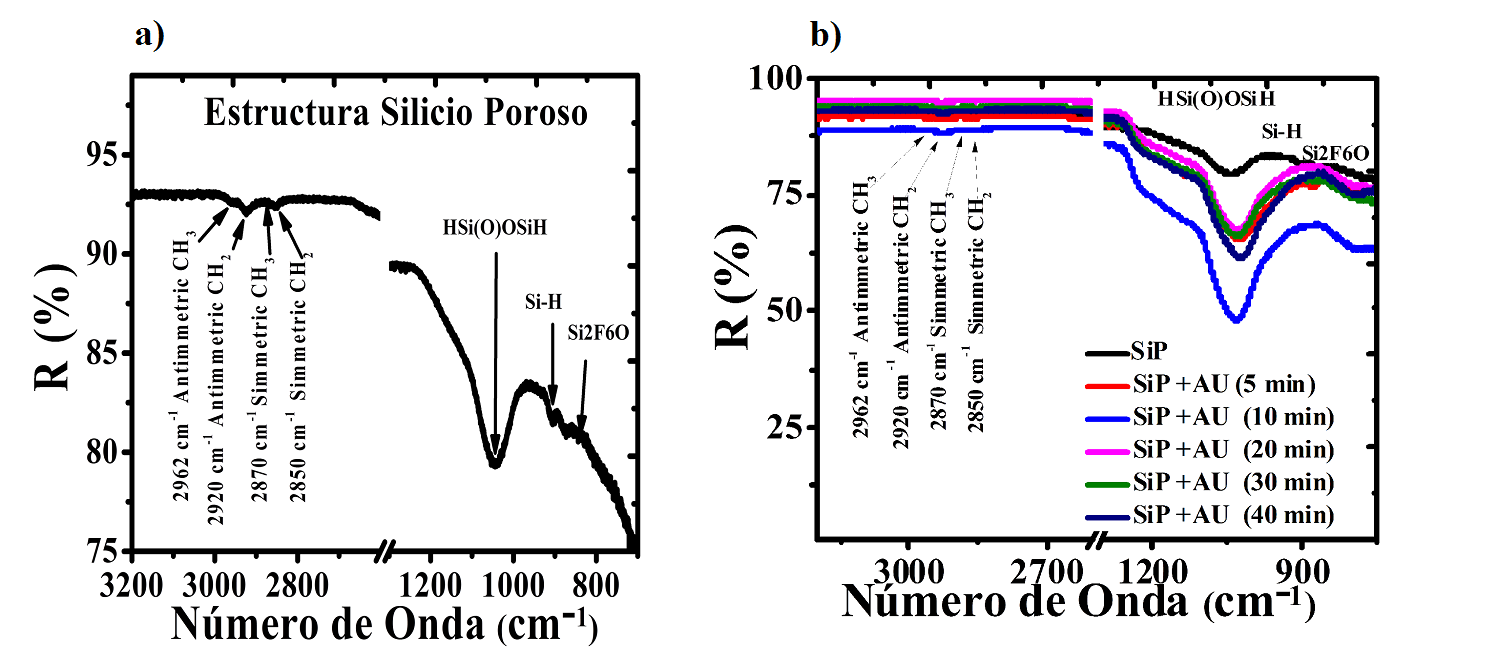
\includegraphics[scale=.32]{../Images/sens2}
	\caption{\emph{Espectro Transmisión Infrarroja de Transformada de Fourier FTIR. a) Muestra un espectro infrarrojo de una superficie recién
		anodizada de silicio poroso. b) La superficies del SiP después de la funcionalización con ácido undeconoico (AU) a diferentes tiempo de tratamiento térmico.}}
	\label{fig:FTIR1}
\end{figure}
La Figura \textbf{\ref{fig:FTIR1} a)} muestra un espectro infrarrojo de una superficie recién anodizada. El espectro muestra picos debidos a los modos de estiramiento Si-O-Si y Si-Si a 2114, 1107 y 621   , respectivamente, y modos de flexión a 908 $cm^{-1}$.
La Figura \textbf{\ref{fig:FTIR1} b)} muestra un espectro infrarrojo de la superficie SiP derivada con ácido undeconoico. Después de la reacción con ácido undeconoico a 180\grad C durante diferentes tiempos(5,10, 20, 30, 40 min), consiste en picos debido al estiramiento y la deformaciónde la cadena de alquilo en 2922 y 1460 $cm^{-1}$, respectivamente. La fuerte absorción a 1712 $cm^{-1}$  es característica del estiramiento carbonilo ($\nu CO$). Sin más información, es difícil asignar inequívocamente este pico a un ácido libre, porque se observó una frecuencia similar para la función carbonilo en los ésteres de sililo\cite{UA1, UA2}.  Sin embargo, la presencia de un pico amplio a 3060 $cm^{-1}$  y la ausencia de carbono-carbono($C=C$).   El doble enlace que se extiende a 1640 $cm^{-1}$  está de acuerdo con un proceso térmico en el que los enlaces de silicio-hidrógeno se agregan selectivamente al enlace doble $C=C$ . Además, la disminución de la intensidad del modo  $Si$-$H_X$  y el cambio insignificante de la intensidad del pico a 1109 $cm^{-1}$ son consistentes con una reacción de hidrosililación que consume enlaces. Esto indica que la mayor parte del consumo fue consumido por una reacción de hidrosililación en lugar de una reacción térmica con el grupo hidroxilo de la función ácida. El IR muestra la presencia de enlaces $Si$-$H_X$ sin reaccionar a 1091 $cm^{-1}$ . Esto se debe al impedimento estérico en la superficie, que limita el consumo completo de todos los nativos $Si$-$H_X$ cautiverio.
La reacción directa del ácido undeconoico con una superficie de SiP terminada en hidrógeno tiene lugar bajo condiciones suaves para producir una monopelicula orgánica unida covalentemente a la superficie a través de los enlaces Si-C. El método térmico es muy conveniente para la introducción de grupos funcionales al final de la monopeliculas, que pueden someterse a manipulaciones químicas adicionales. Sorprendentemente, el grupo funcional ácido terminal no ataca los enlaces de si-si, y la reacción con la superficie ocurre en el terminal  doble enlace. La función ácida
$C$ = $C$ terminal se puede transformar en un éster succinimidílico de una manera muy sencilla y directa.


\begin{figure}[H]
	\centering
	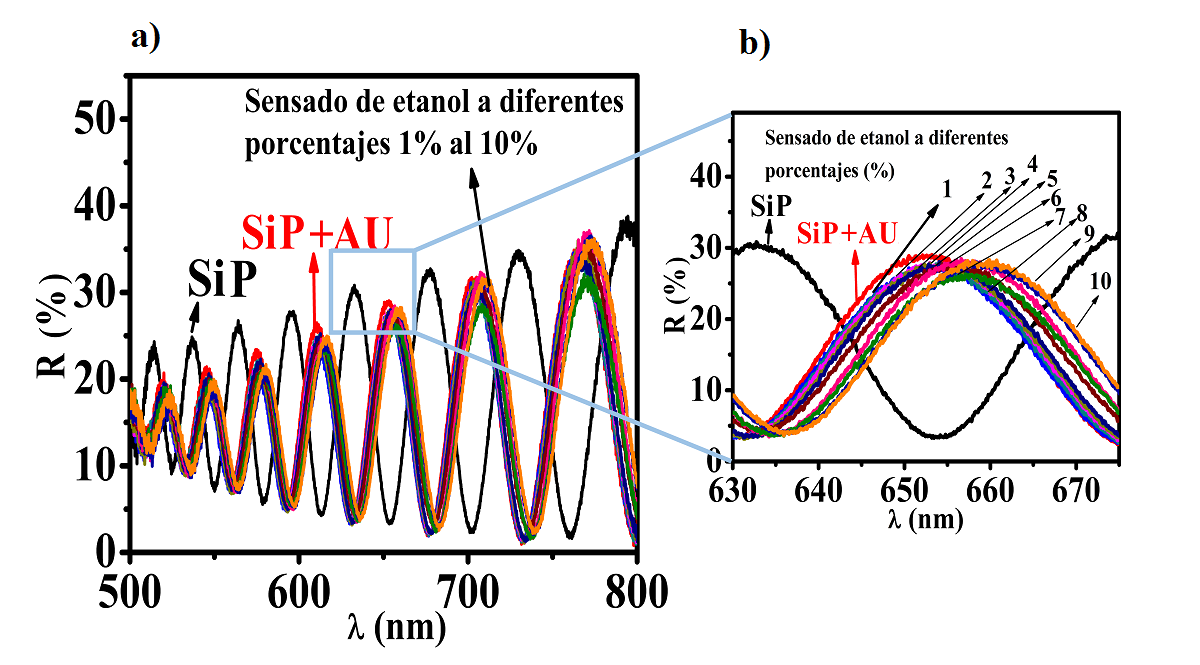
\includegraphics[scale=.4]{../Images/senso01}
	\caption{\emph{E a) Muestra los espectro de reflectancia de la   superficies del SiP después de la funcionalización con ácido undeconoico (AU) a diferentes tiempo de tratamiento térmico mostrando la la detección de etanol al 1$\%$. b) Podemos ver en detalles los porcentajes detestado del 1 al 10 $\%$ de etanol}}
	\label{fig:MCR1}
\end{figure}

\begin{figure}[H]
	\centering
	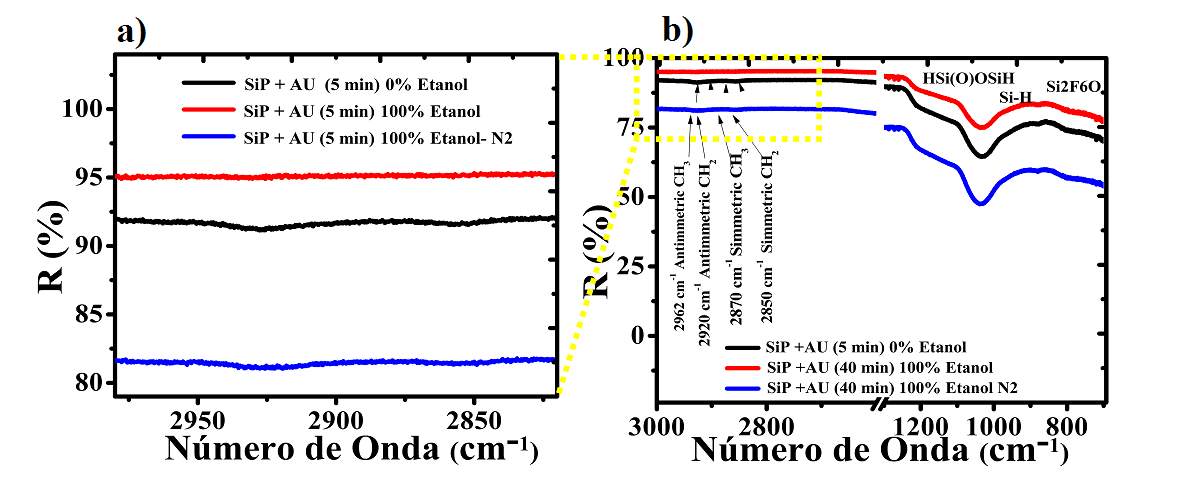
\includegraphics[scale=.4]{../Images/senso2}
\caption{\emph{Espectro Transmisión Infrarroja de Transformada de Fourier FTIR. a) Muestra la superficies del SiP después de la funcionalización con ácido undeconoico (AU) a diferentes tiempo de tratamiento térmico, la detección de etanol al 1$\%$. b) Detallamos los picos de estiramientos simétricos y antisimétricos.}}
\end{figure} 
\subsection{Sensor en microcavidades de silicio poroso con GRIN }
Tomando las consideraciones expuesta de la sección 2.5,  los  datos iniciales para diseño convencional de microcavidades de silicio poroso  utilizamos $\lambda_{_{c}}= 0.67 \mu m$, $n_{_{H}} =2,6$, $P_{_{H}} =0.46$, $d_{_{H}}=0.066 \mu m  $, $t_{_{H}}=35 s  $ y para  $n_{_{L}}= 1,4$,  $P_{_{L}} =0.75$, $d_{_{L}}=0.117 \mu m  $, $t_{_{L}}=11 s  $. 
\begin{figure}[H]
	\centering
	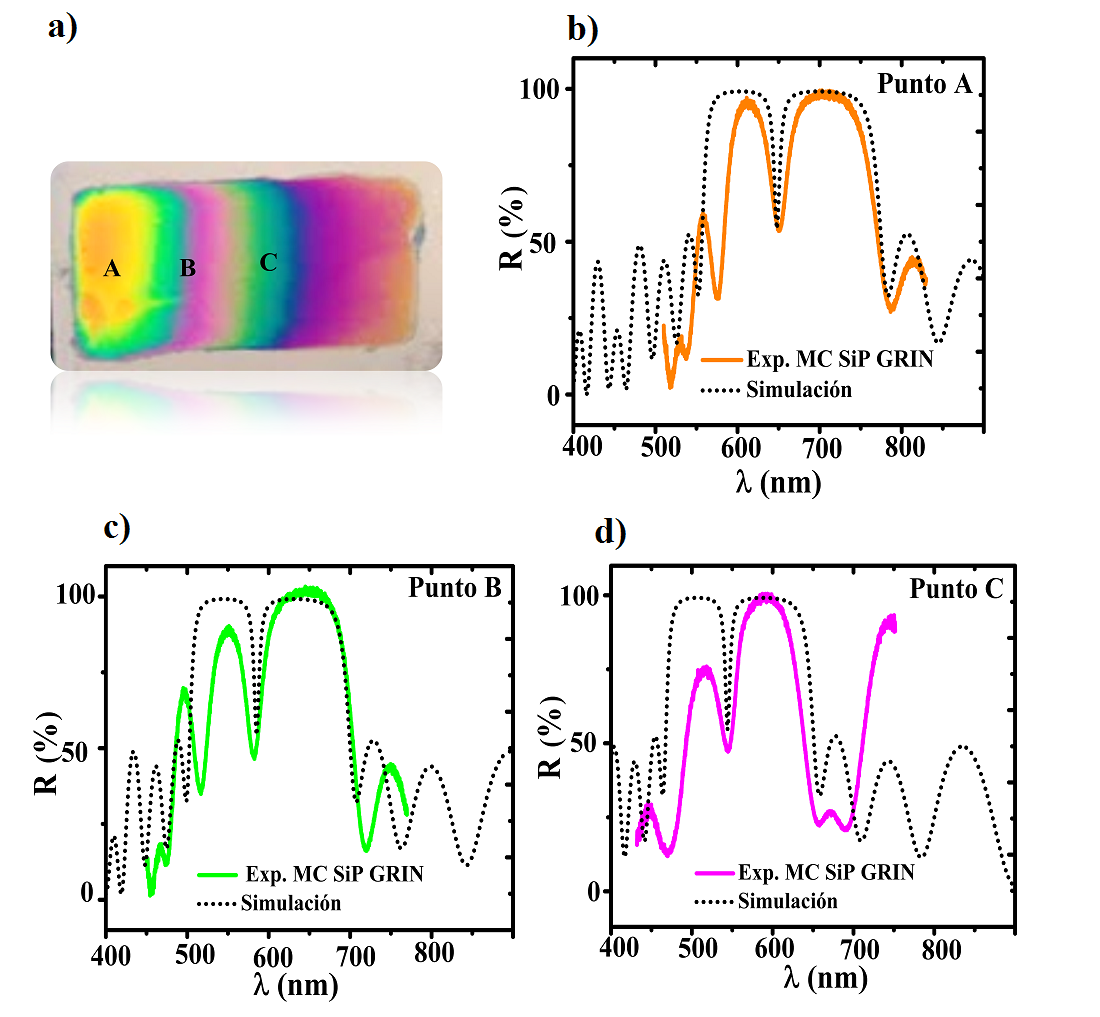
\includegraphics[scale=.3]{../Images/MCGRIN1}
	\caption{\emph{a) Se consideran tres ubicaciones en diferentes puntos denotado de la siguiente forma,  $A(0.3\ \ cm)$ y $ B(0.8 \ \  cm)$ y $ C(1.2 \ \  cm)$, de la  muestra de SiPMCGRIN $GMC$.  b) Para el punto A, c) Para el punto B y d) para el punto C, mostramos los espectro de reflectancias ($\%$) en función de la longitud de onda (nm), de las microcavidades de silicio poroso GRIN,  los datos esta muy acorde la simulación y el experimento, encontramos los indices de refracción y las porosidades en función de la densidad de corriente en cada punto de medición}}
	\label{fig:MCGRIN03}
\end{figure}

En la Figura \textbf{\ref{fig:MCGRIN03} a)} se consideran tres ubicaciones en diferentes puntos denotado de la siguiente forma,  $A(0.3\ \ cm)$ y $ B(0.8 \ \  cm)$ y $ C(1.2 \ \  cm)$, de la  muestra de SiPMCGRIN $GMC$. Las Figuras \textbf{\ref{fig:MCGRIN03} b), c) y d)} mostramos los espectros de reflectancia($\%$) en función de la longitud de onda (nm), para el punto A para  $\lambda_{_{A}}=649 nm$, para el punto B para  $\lambda_{_{B}}=581 nm$ y para el punto C para  $\lambda_{_{C}}=545 nm$, sacamos  los anchos medios de los picos FWHM (Full Width at Half Maximum)\cite{FMHW1, FMHW2, FMHW3} en cada punto de medición  16.4 nm ( en punto A), 18.2 nm ( en punto B) y 22.5 nm ( en punto C)
\begin{figure}[H]
	\centering
	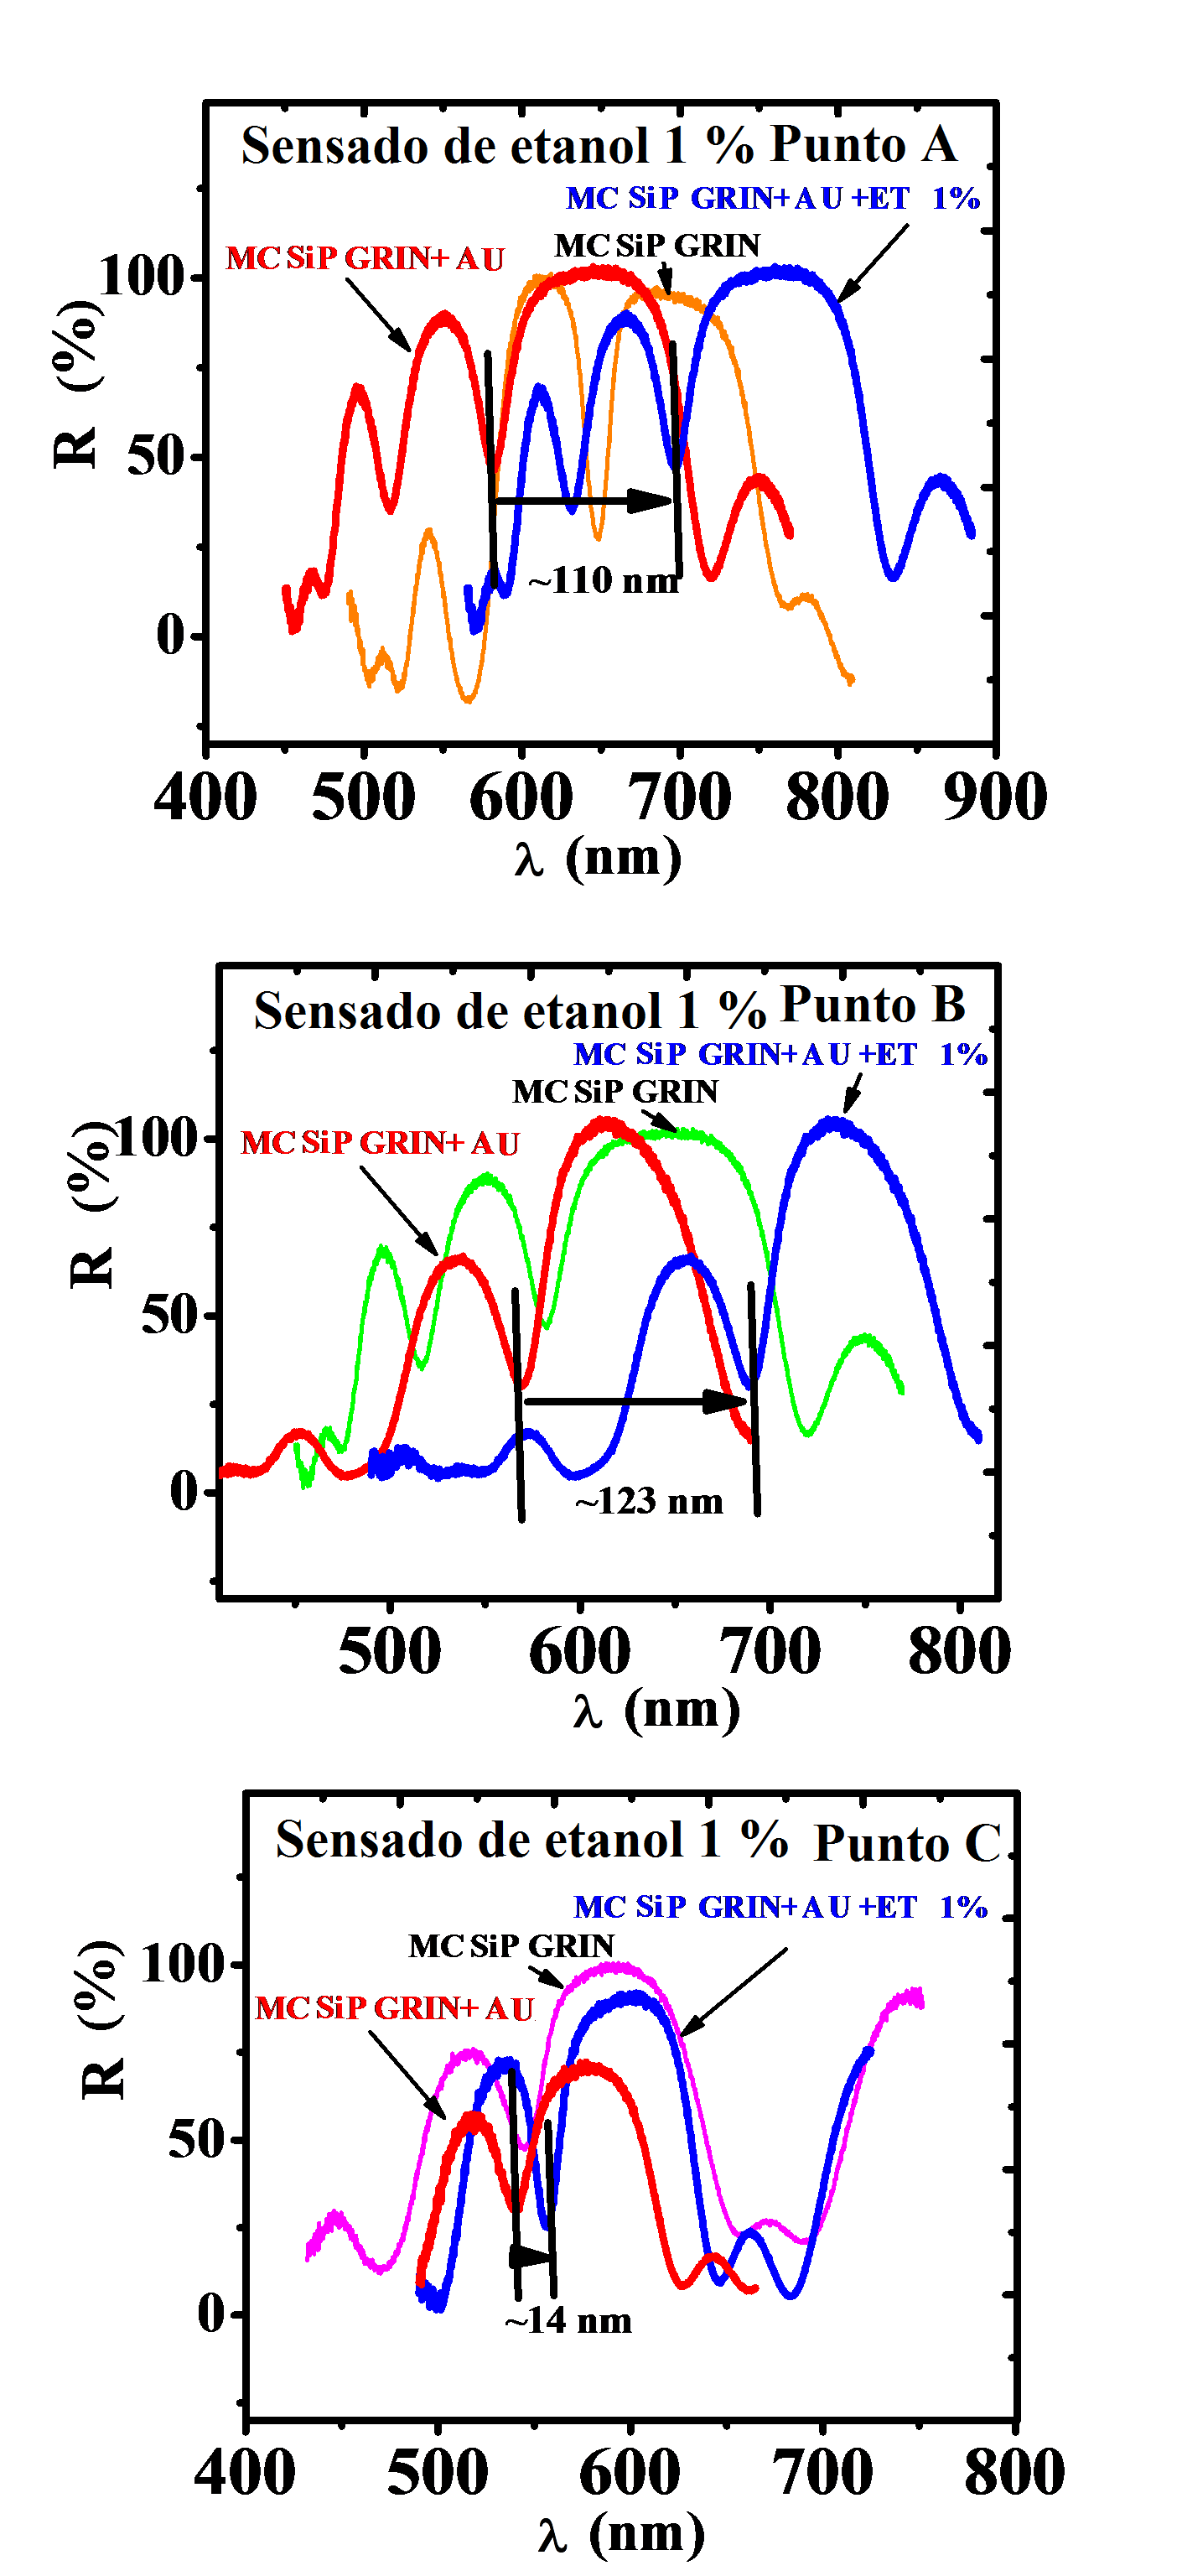
\includegraphics[scale=.18]{../Images/mcsensado}
	\caption{\emph{Espectro de reflectancias ($\%$) en función de la longitud de onda (nm), como se indica en la Figura \ref{fig:MCGRIN03}. a) Comparamos la diferencias de picos en el punto A, $ \lambda(A)_{_{AU}}=585 nm$,  $ \lambda(A)_{_{AU+Et}}=698 nm$ y  $\Delta \lambda(A)_{_{(AU)AU+Et}}=110 nm$. b) Comparamos la diferencias de picos en el punto B,  $ \lambda(B)_{_{AU}}=5569 nm$,  $ \lambda(B)_{_{AU+Et}}=687 nm$ y  $\Delta \lambda(B)_{_{(AU)AU+Et}}=123 nm$.  c) Lo mismo para este punto C,  $ \lambda(C)_{_{AU}}=539 nm$,  $ \lambda(C)_{_{AU+Et}}=554 nm$ y  $\Delta \lambda(C)_{_{(AU)AU+Et}}=14 nm$.  }}
	\label{fig:MCGRIN8}
\end{figure}
En la Figura \textbf{\ref{fig:MCGRIN8}} se muestran los spectro de reflectancias ($\%$) en función de la longitud de onda (nm), como se indica en la Figura \textbf{\ref{fig:MCGRIN03}}. En la \textbf{\ref{fig:MCGRIN8} a)} Comparamos la diferencias de picos en el punto A, $ \lambda(A)_{_{AU}}=585 nm$,  $ \lambda(A)_{_{AU+Et}}=698 nm$ y  $\Delta \lambda(A)_{_{(AU)AU+Et}}=110 nm$. La Figura \textbf{\ref{fig:MCGRIN8} b)} Comparamos la diferencias de picos en el punto B,  $ \lambda(B)_{_{AU}}=5569 nm$,  $ \lambda(B)_{_{AU+Et}}=687 nm$ y  $\Delta \lambda(B)_{_{(AU)AU+Et}}=123 nm$. La figura  \textbf{\ref{fig:MCGRIN8} c)} para el punto C,  $ \lambda(C)_{_{AU}}=539 nm$,  $ \lambda(A)_{_{AU+Et}}=554 nm$ y  $\Delta \lambda(A)_{_{(AU)AU+Et}}=14 nm$.

\begin{figure}[H]
	\centering
	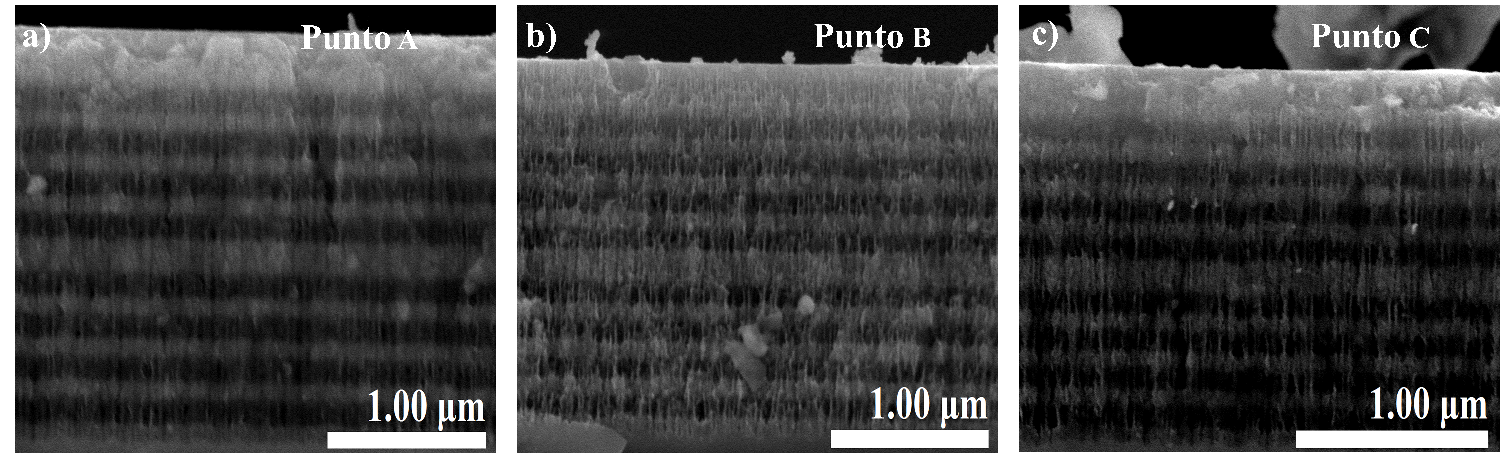
\includegraphics[scale=.3]{../Images/MCSEMSE1}
	\caption{\emph{Imagen SEM del perfil de la sección transversal de las microcavidades con GRIN.}}
	\label{fig:MCGRIN9}
\end{figure}
La Figura \ref{fig:MCGRIN9}. muestra las imágenes transversales de SEM de las muestras de SiP empleadas en este trabajo. Rugosidad de la interfaz relativamente pequeña y un claro contraste entre el alto y bajo porosidad  de la microcavidad medida en diferentes putos (A, B y C), mostrando el cambio de espesores en cada una de estas. 
Los espesores medidos de las estructuras multipeliculas completas mostraron una buena concordancia con las  simulaciones tomado de $V=0.53J^{0.79}$ donde $d_j=Vt_j$ ($j=H,L$), que son los espesores de cada una de la monopelicula de la microcavidad de silicio poroso GRIN en los puntos de medición y el espesor total  lo encontramos como  $d_{_{i}} = (N_{_{Hi}}d_{_{Hi}})+(N_{_{Li}}d_{_{Li}}) + (2d_{_{Hi}})$  definiendo a $i=$ A, B, C. Lo que resultó en (medido / simulación) $2.15 / 2.07 \ \ \mu m $ (para estructura en Punto A), $1.87 / 1.75 \ \ \mu m $ (para estructura en el punto B) y $1.71 / 1.55 \ \ \mu m $ (para estructura  en el punto C). Pudiendo decir que para cada puntos de mediciones le corresponde diferentes densidades de corrientes calculada, lo que corresponden a diferentes espesores al final de la fabricación viendo claramente el gradiente lateral producto de nuestro experimento.
\section{Conclusión}
Presentamos un método sencillo de producción de Silicio poroso de indices de refracción de gradiente; de una microcavidad  graduados lateralmente, que se  puede usar como un sensor óptico para detectar concentraciones extremadamente bajas de soluciones de etanol. Los picos de los espectro de reflectancias ($\%$) en función de la longitud de onda (nm) medidos nos muestras el corrimiento hacia el azul cuando funcionalizamos con ácido undeconoico y después le colocamos el etanol se mueve hacia el rojo detectando concentración del 1$\%$ de etanol para diferentes puntos en una misma muestra. 


%\include{Capitulos/cap1}
\thispagestyle{empty}
%\include{Capitulos/Conclusiones}
\chapter{Conclusiones y Perspectivas}
\thispagestyle{empty}
\subsection{Conclusiones}
Podemos concluir que se derivaron las expresiones necesarias para las componentes del potencial, encontrándonos una relación de la punta del contraelectrodo que actúa análogamente como una carga puntual y la densidad de corriente para una geometría en una caja electrolítica rectangular y resolvemos las ecuaciones electrostática con condiciones de contornos adecuadas. Dando como resultado un modelo electrostático para cristales con índice de refracción con gradiente (MECFGRIN).
Es la primera vez que el formalismo aquí mencionado se aplica para encontrar la densidad de corriente para diseñar silicio poroso. La forma del electrodo, el Área de la celda  produce una visible disminución en el tamaño y densidad de los poros. Adicionalmente,  optimizando las propiedades estructurales para una solo estructura pudimos tener un gradiente con diferentes profundidades, reflactancias en diferentes  punto de medición. De ese modo, pudimos simular la relación directa de la velocidad de ataque con la densidad de corrientes en los punto de la muestras de interés. A la vez desarrollamos una caracterización entre porosidad, índices de refracción del silicio poroso, con las diferentes densidades de corrientes. Con todo esto pudimos  usar estas microcavidades  como un sensor óptico para detectar concentraciones extremadamente bajas de soluciones de etanol. Los picos de los espectro de reflectancias ($\%$) en función de la longitud de onda (nm) medidos nos muestras el corrimiento hacia el azul cuando funcionalizamos con ácido undeconoico y después le colocamos el etanol se mueve hacia el rojo detectando concentración del 1$\%$ de etanol para diferentes puntos en una misma muestra. 

\subsection{Perspectivas y recomendaciones}
Esperamos que estas investigaciones sean aplicadas para diseñar un nuevo tipo de switch óptico basados en estructuras de multicapas porosas donde en una sola muestra pueda tener diferentes propiedades para filtrar, los tamaños de poros y porosidad, donde sea posible el sensado de diferentes moléculas. Además, el entendimiento de las propiedades ópticas de estos sistemas puedan ser útiles en el diseño de novedosos dispositivos donde sea posible modular la propagación de ondas electromagnéticas en el orden de los Terahertz para aplicaciones biomédicas. También una gran opción para fabricar  los catalizadores híbridos que  son altamente estables (químicos y térmicos), tienen un buen rendimiento de reutilización y pueden utilizarse de manera eficiente para detectar contaminantes como  4-NP ( 4-nitrofenol). 
\newpage
%----------------------------------------------------------------------------------------
%	APÉNDICES
%----------------------------------------------------------------------------------------

%\addtocontents{toc}{\vspace{2em}} % Agrega espacios en la toc

\appendix % Los siguientes capítulos son apéndices

 % Incluye los apéndices en el folder de apéndices

%\include{Apendices/Ap}
%\thispagestyle{empty}
%\include{Apendices/AppendixB}
%\include{Apendices/AppendixC}

\chapter{Modelo MECFGRIN}\label{aped.A}
\section{Complemento Teórico }


La Figura \textbf{\ref{fig:TA}}   tenemos es una fuente puntual igual que los casos de la electrostática, para una delta de Dirac un conductor perfecto, para generar un campo equipotencial. Sucede que va haber una replicas de la fuentes en los planos, el cual podemos evaluar con una descomposición de Fourier. Tendríamos métodos de imágenes  considerando lo siguiente: $\vec{J}=\sigma \vec{E}$ densidad de corriente donde $\sigma$ conductividad del electrolito y $\vec{E}$ el campo eléctrico producido por la corriente electrostática. Siendo $\nabla^2 \cdot \vec{J}= -\dfrac{\partial \rho}{\partial t}=0$ para corrientes estacionarias.
Ahora podemos relacionar $\vec{J}= \frac{I}{4\pi r^2}\hat{r}=\sigma \vec{E}$ quedando la carga en igual a la corriente y proporcional a la conductividad $q = \frac{I}{4\pi \sigma}$.


\begin{figure}[H]
	\centering
	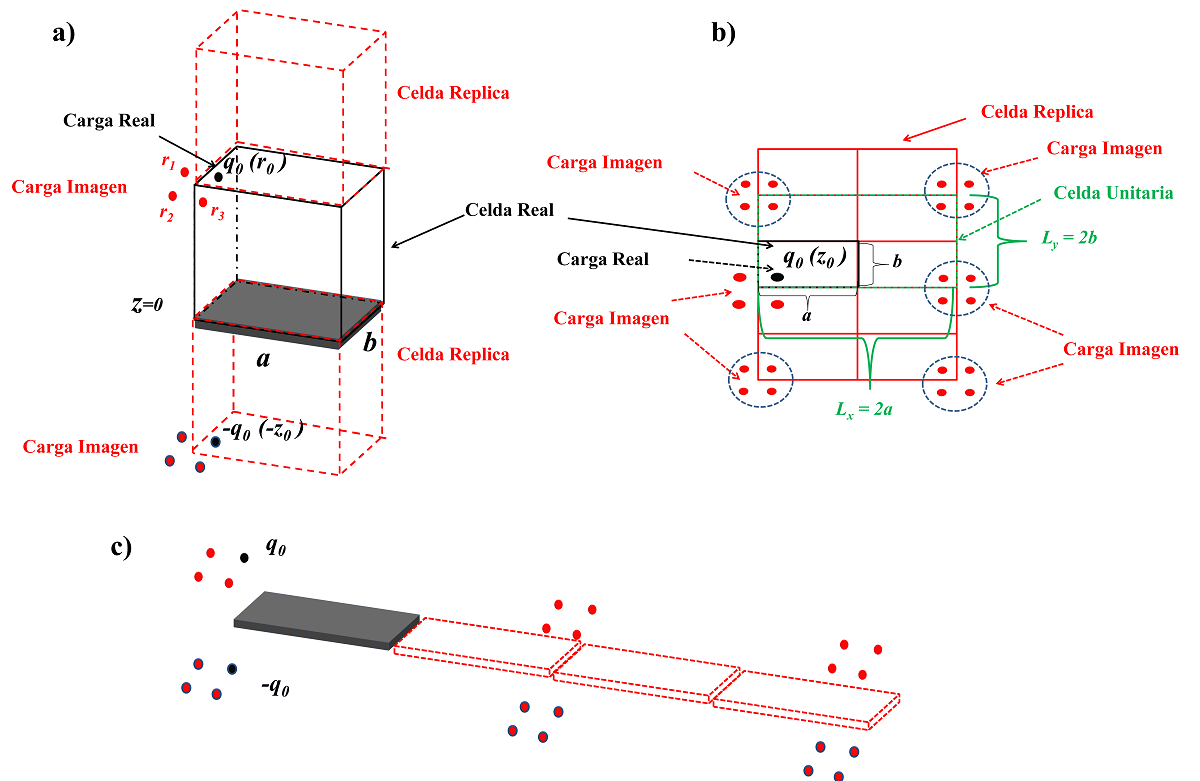
\includegraphics[scale=.4]{../Images/Cellgrin}
	\caption{\emph{a)Esquema de una celda electrolítica rectangular, con una carga real en la esquina de la celda con sus cargas ($q$) imágenes de  igual signo en $Z_0$ y otra carga imagen ($-q$) con cambio de signo  ubicada debajo del  conductor en la posición $-Z_0$. b)La cara superior vista desde arriba, una carga real y sus cargas imágenes  en el $Z_0$. c) Todo esto formado un  sistemas de una carga real y sus  cargas imágenes producidas por las paredes de la celda y sus otras imágenes  vista desde arriba, formando un espacio periódicos. }}
	\label{fig:TA}
\end{figure}
En la Figura \textbf{\ref{fig:TA}}  nos muestra el arreglo periódico que  es principalmente matemático y se refiere a la forma precisa de la interacción de la corriente estacionaria apropiada para los cálculos de dos dimensiones. Podemos señalar las coordenadas de la fuente la puntual $\vec{r_0}= (x_0, y_0, z_0)$ y sus replicas $\vec{r_1}= (-x_0, y_0, z_0)$, $\vec{r_2}= (-x_0, -y_0, z_0)$ y $\vec{r_3}= (x_0, -y_0, z_0)$ para $\vec{r_j}$, $(j=0,1,2,3)$. La dirección periódica es $z$ y la celda unitaria es de longitud $2L_x$ y $2L_y$, y las copias periódicas separadas por vacío en el plano $xy$ cuya área se está incrementando para lograr la convergencia. 

\begin{eqnarray}
\nonumber \varphi(r) &=& \varphi(x,y,z)\\
\varphi(x,y,z)&=& \varphi(x+2L_x,y+2L_y,z)
\end{eqnarray}


\begin{eqnarray}
\nonumber \rho(x,y,z) &=&  \displaystyle\sum_{j} q  \ \delta (r-r_j-(2L_x \hat{x} +2L_y \hat{y})) \\
\rho(x,y,z) &=& \displaystyle\sum_{j} q  \ \delta (x-x_j-2L_x) \ \delta(y-y_j-2L_y) \ \delta (z-z_0)
\end{eqnarray}

Tenemos un arreglo periódico con un vector periódico $\vec{a}= (2L_x,2L_y) $ y expandiendo en series de Fourier este sistema queda, para el caso del potencial.
\begin{eqnarray}
\varphi(x,y,z)= \displaystyle\sum_{G_x} \displaystyle\sum_{G_y} \varphi_{_{G_x G_y}} e^{iG_x x}e^{iG_y y}
\end{eqnarray}
En lo que sigue, nos centraremos principalmente en una red rectangular en el plano $xy$, por lo que $A = 4 L_x  L_y$. Los vectores recíprocos en el plano $xy$ se llaman $G_{i} = 2 \pi (n_i)/ a_i$, ($i= x,y$), la proyección del vector de posición en el plano $xy$ es $r_{\Vert}$, y los vectores recíprocos a lo largo de $z$ son $G_z = 2\pi j / L$ para entero j. A menudo acortaremos la longitud de $r_{\Vert}$ como r, entonces $\vec{r} = \vert {r_{\Vert} } \vert =\sqrt{x^2 + y^2} $. Y $G =(G_x, G_y) $ y su tamaño $ \vert G \vert =\sqrt{G^2_x+ G^2_y} $ 
\begin{eqnarray}
\varphi(x,y,z)= \displaystyle\sum_{G\neq 0}  \varphi_{_{G}} e^{iG r_{\Vert}}
\end{eqnarray}
\subsection{Caso 1 para $z_0$}
Considerando la ecuación de Poisson 
\begin{eqnarray}
\nabla^2 \varphi(x,y,z)= -4 \pi \rho(x,y,z)
\end{eqnarray}
Resolvemos la ecuación 
\begin{eqnarray}
\nabla^2 \varphi(x,y,z)= \displaystyle\sum_{G \neq 0} \Bigg(\dfrac{\partial^2 \varphi_{_{G}}(z)e^{iG r_{\Vert} }}{\partial x^2}+ \dfrac{\partial^2 \varphi_{_{G}}(z)e^{iG r_{\Vert}}}{\partial y^2}+\dfrac{\partial^2 \varphi_{_{G}}(z)e^{iG r_{\Vert}}}{\partial z^2} \Bigg)=0
\end{eqnarray}
Realizamos las derivadas de las ecuación anterior, y para algunos planos no existen cargas por lo que podemos igualar a cero.
\begin{eqnarray}
\displaystyle\sum_{G \neq 0} \Bigg(G^{2}_{x} \varphi_{_{G}}(z)e^{iG r_{\Vert}} + G^{2}_{y}\varphi_{_{G}}(z)e^{iG r_{\Vert}}+ \dfrac{d^2 \varphi_{_{G}}(z)}{d z^2} e^{iG r_{\Vert}} \Bigg)=0 \\
\displaystyle\sum_{G \neq 0} \Bigg(G^2_x \varphi_{_{G}}(z) + G^2_y\varphi_{_{G}}(z)+ \dfrac{\partial^2 \varphi_{_{G}}(z)}{\partial z^2} \Bigg)e^{iG r_{\Vert}}=0\\
(G^2_x + G^2_y)\varphi_{_{G}}(z)+ \dfrac{\partial^2 \varphi_{_{G}}(z)}{\partial z^2}=0\\
G^2\varphi_{_{G}}(z)+ \dfrac{\partial^2 \varphi_{_{G}}(z)}{\partial z^2}=0
\end{eqnarray}

\begin{eqnarray}
\dfrac{\partial^2 \varphi_{_{G}}(z)}{\partial z^2}+ G^2\varphi_{_{G}}(z)=0
\end{eqnarray}

La solución depende de donde se este evaluando el potencial en $z_0$ para puntos cercanos hacia arriba hacia abajo, $z_1$ y $z_2$, así como se describe en la Figura \textbf{\ref{fig:TA} }

\begin{eqnarray}
\varphi_{_{G}}(z)=A_{_G}  e^{G z} + B_{_G}  e^{-G z} \ \ \ \ \ \ \ \ z<z_0 \\
\varphi_{_{G}}(z)=C_{_G}  e^{G z} + F_{_G}  e^{-G z} \ \ \ \ \ \ \ \ z>z_0
\end{eqnarray}


%\begin{eqnarray*}
%	\varphi_{_{G}}(z)&=& A_{_G}  e^{G z} + \cancel{B_{_G}  e^{-G z}} \ \ \ \ \ \ \ \ z<z_0 \ \ \ \ \ \ \ \ z \rightarrow - \infty \\
%	\varphi_{_{G}}(z)&=&  \cancel{C_{_G}  e^{G z}} + F_{_G}  e^{-G z} \ \ \ \ \ \ \ \ z>z_0 \ \ \ \ \ \ \ \ z \rightarrow \infty
%\end{eqnarray*}

Según estas consideraciones las soluciones son simétricas, 

\begin{eqnarray*}
	\varphi(z_2)&=& A_{_G}  e^{G z_2} = A_{_G}  e^{G (2z_0-z_1)}\\
	\varphi(z_1)&=& F_{_G}  e^{G z_1} \\
	F_{_G}  e^{G z_1}&=& A_{_G}  e^{G (2z_0-z_1)}\\
	F_{_G} & =& A_{_G}  e^{G (2z_0)}
\end{eqnarray*}
Redefinimos las variables 
\begin{eqnarray*}
	H_{_G} & =& F_{_G}  e^{-G (z_0)}\\
	F_{_G} & =& H_{_G}  e^{G (z_0)}\\
	A_{_G} & =& F_{_G}  e^{-G (2z_0)}\\
	A_{_G} &=& H_{_G} e^{G (z_0)} e^{-G (2z_0)}=H_{_G} e^{-G (z_0)}\\
	A_{_G} &=& H_{_G} e^{-G (z_0)}   
\end{eqnarray*}
Las soluciones nos queda simétrica

\begin{eqnarray*}
	\varphi_{_{G}}(z)&=& H_{_G}  e^{-G z_0} e^{G z} \ \ \ \ \ \ \ \ z<z_0 \\
	\varphi_{_{G}}(z)&=& H_{_G} e^{G z_0} e^{-G z} \ \ \ \ \ \ \ \ z>z_0
\end{eqnarray*}

\begin{eqnarray*}
	\varphi_{_{G}}(z)&=& H_{_G}  e^{G (z-z_0)}  \ \ \ \ \ \ \ \ z<z_0 \\
	\varphi_{_{G}}(z)&=& H_{_G} e^{G (z_0-Z)} \ \ \ \ \ \ \ \ z>z_0
\end{eqnarray*}

\begin{eqnarray}
\varphi_{_{G}}(z) &=& H_{_G}  e^{-\vert G \vert \vert z-z_0 \vert}  
\end{eqnarray}

Ahora evaluamos cuando $G=0$
\begin{eqnarray}
\varphi''_{_{_{G=0}}}(z) &=& 0\\
\varphi_{_{G}}(z) &=& \varphi_{_{0}} +A_0 \vert z-z_0 \vert
\end{eqnarray}

Hacemos la segunda parte de la solución para, también expandimos con series de Fourier,
\begin{eqnarray}
\nonumber \rho(x,y,z) &=&  \displaystyle\sum_{j} q  \ \delta (r-r_j-(2L_x \hat{x} +2L_y \hat{y})) \\
\rho(x,y,z) &=& \displaystyle\sum_{j} q  \ \delta (x-x_j-2L_x) \ \delta(y-y_j-2L_y) \ \delta (z-z_0)\\
\nonumber \rho(x,y,z) &=&\delta (z-z_0) \displaystyle\sum_{G} \sigma_{G} e^{i G r_{\Vert}}
\end{eqnarray}
\begin{eqnarray}
\nonumber  \displaystyle\sum_{j} q  \ \delta (x-x_j-2L_x) \ \delta(y-y_j-2L_y) \ \delta (z-z_0) &=&\\\delta (z-z_0) \displaystyle\sum_{G} \sigma_{G} e^{i G r_{\Vert}}
\end{eqnarray}
Integro sobre el Área de la celda unitaria $\int \frac{d^2r_{\Vert}}{A} e^{i G^{'} r_{\Vert}}$
\begin{eqnarray}
\nonumber \int \frac{d^2r_{\Vert}}{A} \Bigg( \displaystyle\sum_{j} q  \ \delta (x-x_j-2L_x) \ \delta(y-y_j-2L_y) \ \delta (z-z_0) &=&\\\delta (z-z_0) \displaystyle\sum_{G} \sigma_{G} e^{i G r_{\Vert}} \Bigg)e^{-i G^{'} r_{\Vert}}
\end{eqnarray}

\begin{eqnarray}
\nonumber  \displaystyle\sum_{G} \sigma_{_{G}} \delta_{_{GG'}} &=&\frac{q}{A} e^{-i G^{'} r_{j}}\\
\sigma_{_{G}}  &=&\frac{q}{A} e^{-i G r_{j}}
\end{eqnarray}
Ya podemos escribir el potencial completo
\begin{eqnarray}
\varphi(x,y,z)= \varphi_{_{0}} +A_0 \vert z \vert + \displaystyle\sum_{G\neq 0} H_{_G}  e^{-\vert G \vert \vert z \vert}  e^{i G r_{\Vert}}
\end{eqnarray}

Hasta aquí tengo en potencial completo, queda solo por calcular las variables $A_0$ y $ H_{_G} $, por lo que vamos a utilizar la discontinuidad del campo eléctrico definido así, $ \vec{E}= -\nabla \varphi $

\begin{eqnarray}
\vec{E_{z}}(0^+) &=& -A_0  - \displaystyle\sum_{G\neq 0} H_{_G}(+G)  e^{i G r_{\Vert}}\\
\vec{E_{z}}(0^-) &=& A_0  + \displaystyle\sum_{G\neq 0} H_{_G}(-G)  e^{i G r_{\Vert}}
\end{eqnarray}
Con los campos y su discontinuidad 
\begin{eqnarray}
\Delta \vec{E_{z}} &=& -2A_0  + 2 \displaystyle\sum_{G\neq 0} (G) H_{_G}  e^{i G r_{\Vert}}=4\pi \sigma_{_{G}}
\end{eqnarray}
Como son coeficientes de Fourier son iguales por la queda es,
\begin{eqnarray}
4\pi \sigma_{_{G}}=\frac{4\pi}{A} e^{-i G r_{j}}e^{i G r_{\Vert}}
\end{eqnarray}
\begin{eqnarray}
\nonumber -2A_0&=&\frac{4\pi q}{A} \\
A_0&=& -\frac{2\pi q}{A}
\end{eqnarray}

\begin{eqnarray}
\nonumber 2GH_{_G}&=&\frac{2\pi q}{A}e^{-i G r_{j}} \\
H_{_G} &=&\frac{2\pi q}{AG}e^{-i G r_{j}}
\end{eqnarray}
El potencial completo considerando el punto donde se avalúa el potencial nos queda de la siguiente forma:

\begin{eqnarray}
\varphi(x,y,z)= \varphi_{_{0}} -\frac{2\pi q\vert z-z_0 \vert}{A}  + \frac{2\pi q}{A}\displaystyle\sum_{G\neq 0}  \frac{ e^{-\vert G \vert \vert z-z_0 \vert} }{\vert G \vert} e^{i G \cdot(r_{\Vert}-r_{j})}
\end{eqnarray}

Consideramos 
\begin{eqnarray}
q = \frac{I}{4\pi \sigma}\\
\varphi\rightarrow \vec{E_z}(z=0)\\
J_z(z=0)=\sigma \vec{E_z}(z=0^+)
\end{eqnarray}
\subsection{Caso 2 para $-z_0$}
Tomando de la Figura \textbf{\ref{fig:TA}}, el potencial completo considerando el punto donde se avalúa el potencial nos queda de la siguiente forma:

\begin{eqnarray}
\varphi(x,y,z)= \varphi_{_{0}} +\frac{2\pi q\vert z+z_0 \vert}{A}  - \frac{2\pi q}{A}\displaystyle\sum_{G\neq 0}  \frac{ e^{-\vert G \vert \vert z+z_0 \vert} }{\vert G \vert} e^{i G \cdot(r_{\Vert}-r_{j})}
\end{eqnarray}

Consideramos 
\begin{eqnarray}
q = \frac{I}{4\pi \sigma}\\
\varphi\rightarrow \vec{E_z}(z=0)\\
J_z(z=0)=\sigma \vec{E_z}(z=0^-)
\end{eqnarray}









%%----------------------------------------------------------------------------------------
%	BIBLIOGRAFÍA
%----------------------------------------------------------------------------------------
\backmatter
\nocite{*}
%\bibliographystyle{plain}
%\bibliography{bibliografía.bib} %Aquí ponen el nombre del archivo .bib
\bibliographystyle{unsrt}
 \small{
\begin{thebibliography}{X}
\bibitem{Morkoc} H. Morkoç, “\emph{Nitride Semiconductors and Devices}", (Springer, 1999).

\bibitem{I1} P. Yeh,\textquotedblleft Optical Waves in Layered Media \textquotedblright, 2nd edn. (Wiley-Interscience Publication,
USA, 2005).
\bibitem{I2}Canham, L. 1997.\textquotedblleft \emph{Properties of Porous Silicon}  \textquotedblright. Edited by Canham L. DERA, Malvern, UK.
\bibitem{I3}{Beale, M.I.J, J.D Benjamin, M.J Uren, N.G Chew, and A.G Cullis. 1985. \emph{ \textquotedblleft An Experimental and Theoretical Study of the Formation and Microstructure of Porous Silicon.\textquotedblright} J. Crystal Growth 73: 622?36. doi:10.1021/jp0706984. }
\bibitem{I4}Canham, L. T. 1990. \emph{\textquotedblleft Silicon Quantum Wire Array Fabrication by Electrochemical and Chemical Dissolution of Wafers.\textquotedblright } Applied Physics Letters 57 (10): 1046. doi:10.1063/1.103561.


\bibitem{I5} J. D. Joannopoulos et al.,\textquotedblleft Photonic Crystals: Molding the Flow of Light, 2nd edn.
(Princeton University Press, UK, 2008).
\bibitem{I6} E. Yablonovitch, \textquotedblleft Photonic band-gap structures,\textquotedblright J. Opt. Soc. Am. B 10, 283-295 (1993)
\bibitem{I7} S. Ilyas et al., Opt. Mater. 29, 619 (2007).
\bibitem{I8} P. Tran, Opt. Lett. 21(15), 1138 (1996).
\bibitem{I9} A. D. Ariza-Flores et al., Appl. Phys. Lett. 101(3), 031119 (2012).
\bibitem{I10} S. G. Johnson et al., Phys. Rev. B 62(12), 8212 (2000).

%asimetrica 
\bibitem{I101}Collins, Boyce E., et al. \textquotedblleft Determining protein size using an electrochemically machined pore gradient in silicon.\textquotedblright Advanced Functional Materials 12.3 (2002): 187-191.
\bibitem{I102} Khung, Y. L., G. Barritt, and N. H. Voelcker. \textquotedblleft Using continuous porous silicon gradients to study the influence of surface topography on the behaviour of neuroblastoma cells. \textquotedblright Experimental cell research 314.4 (2008): 789-800.
\bibitem{I103} Clements, Lauren R., et al. \textquotedblleft Mesenchymal stem cell attachment to peptide density gradients on porous silicon generated by electrografting.\textquotedblright physica status solidi (a) 208.6 (2011): 1440-1445.
\bibitem{I104} Wang, Peng-Yuan, et al. \textquotedblleft Screening the attachment and spreading of bone marrow-derived and adipose-derived mesenchymal stem cells on porous silicon gradients.\textquotedblright Rsc Advances 2.33 (2012): 12857-12865.
\bibitem{I11} Canham, L. \textquotedblleft Properties of Porous Silicon.\textquotedblright Edited by Canham L. DERA, Malvern, UK. (1997).
\bibitem{I12} Li, Yang Yang, Peter Kim, and Michael J Sailor.\textquotedblleft Painting a Rainbow on Silicon A Simple Method to Generate a Porous Silicon Band Filter Gradient \textquotedblright Physica Status Solidi (a) 1618 (8): 161618. doi:10.1002/pssa.200461200.(2005)
\bibitem{I13} Khung, Y L, and N H Voelcker. 2009.\textquotedblleft Multidirectional Lateral Gradient Films with Position-Dependent Photonic Signatures Made from Porous Silicon. \textquotedblright Optical Materials 32 (1): 23442. doi:10.1016/j.optmat.2009.07.015. 
\bibitem{I14}  Khung, Y L, G Barritt, and N H Voelcker.  \textquotedblleft Using Continuous Porous Silicon Gradients to Study the Influence of Surface Topography on the Behaviour of Neuroblastoma Cells.\textquotedblright Experimental Cell Research 314 (4): 78900. doi:10.1016/j.yexcr.2007.10.015.(2008.)
\bibitem{I15} Collins, B.E., K.-P.S. Dancil, G. Abbi, and M.J. Sailor. 2002.\textquotedblleft Determining Protein Size Using an Electrochemically Machined Pore Gradient in Silicon.\textquotedblright Advanced Functional Materials 12 (3): 187. doi:10.1002/1616-3028(200203)12:3,187::AID-ADFM187,3.0.CO;2-E.( 2002.)

\bibitem{I16} Ocier, C. R., Krueger, N. A., Zhou, W. and  Braun, P. V. \textquotedblleft Tunable visibly transparent optics derived from porous silicon.\textquotedblright ACS Photonics, 4(4), 909-914. (2017).

\bibitem{I17} Dariani RS, Ebrahimnasab S  \textquotedblleft Root Mean Square Roughness of Nano Porous Silicon by Scattering Spectra.\textquotedblright The European Physical Journal Plus 129: 129. (2014).
\bibitem{I18} Lerondel G, Romestain R \textquotedblleft Roughness of the Porous Silicon Dissolution Interface.\textquotedblright Journal of Applied Physics 81:  6171?6178. (1997).
\bibitem{I19} Lérondel G, Romestain R, Barret S \textquotedblleft Quantitative Analysis of the Light Scattering Effect on Porous Silicon 
Optical Measurements.\textquotedblright Thin Solid Films 297: 114?117. (1997).

\bibitem{I20} Thei, W. \textquotedblleft Optical Properties of porous silicon. \textquotedblright Surf. Sci. Rep. 1997, 29, 91?93. 
\bibitem{I21} Van Groesen, E.; Sopaheluwakan, A.; Andonowati, A. \textquotedblleft  Direct characterization of states and modes in defect grating structures. \textquotedblright J. Nonlinear Opt. Phys. Mater. 2004, 13, 155?173. 
% \textquotedblleft \textquotedblright
\bibitem{In} C.Mazzoleni, and L.Pavesi, Appl. Phys. Lett. 67, 2983, (1995).
%CAPITULO 3 MICROCAVIDADES DE ANODIZACION 
\bibitem{I1}{Beale, M.I.J, J.D Benjamin, M.J Uren, N.G Chew, and A.G Cullis. 1985. \emph{?An Experimental and Theoretical Study of the Formation and Microstructure of Porous Silicon.?} J. Crystal Growth 73: 622?36. doi:10.1021/jp0706984. }
\bibitem{I2}{Bisi, O., Stefano Ossicini, and L. Pavesi. 2000. \emph{?Porous Silicon: A Quantum Sponge Structure for Silicon Based Optoelectronics.?} Surface Science Reports 38 (1): 1?126. doi:10.1016/S0167-5729(99)00012-6.}

\bibitem{I3}Canham, L. 1997. \emph{Properties of Porous Silicon}. Edited by Canham L. DERA, Malvern, UK.


\bibitem{Ik}Khung, Y. L., G. Barritt, and N. H. Voelcker. \emph{Using continuous porous silicon gradients to study the influence of surface topography on the behaviour of neuroblastoma cells.} Experimental Cell Research 314.4 (2008): 789-800.
\bibitem{I4}Khung, Y L, G Barritt, and N H Voelcker. 2008. ?Using Continuous Porous Silicon Gradients to Study the Influence of Surface Topography on the Behaviour of Neuroblastoma Cells.? Experimental Cell Research 314 (4): 789?800. doi:10.1016/j.yexcr.2007.10.015.
\bibitem{I5}Li, Yang Yang, Peter Kim, and Michael J Sailor. 2005. ?Painting a Rainbow on Silicon ? A Simple Method to Generate a Porous Silicon Band Filter Gradient? Physica Status Solidi (a) 1618 (8): 1616?18. doi:10.1002/pssa.200461200.
\bibitem{I6}Khung, Y L, and N H Voelcker. 2009. ?Multidirectional Lateral Gradient Films with Position Dependent Photonic Signatures Made from Porous Silicon.? Optical Materials 32 (1): 234?42. doi:10.1016/j.optmat.2009.07.015. 
\bibitem{I7} Wang,  Peng-Yuan,  Lauren  R.  Clements,  Helmut  Thissen,  Andrew  Jane, Wei-Bor  Tsai,  and Nicolas  H.  Voelcker.  2012.   ?Screening   Mesenchymal  Stem  Cell  Attachment  and Differentiation  on  Porous Silicon Gradients.?  Advanced  Functional Materials  22 (16): 3414?23. doi:10.1002/adfm.201200447. Warwick, Michael E A, and Russell Binions. 2014
\bibitem{I8}Lehmann, Volker. 2002. Electrochemistry of Silicon: Instrumentation, Science, Materials and
Applications. Transport. Vol. 3. doi:10.1002/3527600272.ch2.


\bibitem{I9} Chuang, S. F., S. D. Collins, and R. L. Smith. 1989.\emph{ ?Preferential Propagation of Pores during the Formation of Porous Silicon: A Transmission Electron Microscopy Study.?} Applied Physics Letters 55 (7): 675?77. doi:10.1063/1.101819.
\bibitem{I10} Collins, B.E., K.-P.S. Dancil, G. Abbi, and M.J. Sailor. 2002. \emph{?Determining Protein Size Using an Electrochemically Machined Pore Gradient in Silicon.}? Advanced Functional Materials 12 (3): 187. doi:10.1002/1616-3028(200203)12:3<187::AID-ADFM187>3.0.CO;2-E.

\bibitem{I10L}Ocier, Christian R., et al. "Tunable visibly transparent optics derived from porous silicon." ACS Photonics 4.4 (2017): 909-914.
%capitulo 2 fomarmacion
\bibitem{109}Porous Silicon: material processing, properties and applications, France Telecom-CNET, BP. 98, 38243 Meylan cedex, France. 1994.
\bibitem{110} Smith, R. L. "SD collins,“Porous silicon formation mechanisms,”." J. Appl. Phys 71.8 (1992): R1-R22.
\bibitem{112}Lehmann, V., and Ulrich Gösele. "Porous silicon formation: A quantum wire effect." Applied Physics Letters 58.8 (1991): 856-858.
\bibitem{113} Fauchet, Philippe M. "Photoluminescence and electroluminescence from porous silicon." Journal of Luminescence 70.1-6 (1996): 294-309.
\bibitem{114} Ouyang, Huimin, et al. "Microcavidades macroporosas de silicio para la detección de macromoléculas". Materiales funcionales avanzados 15.11 (2005): 1851-1859.

\bibitem{FMHW1} Vinegoni, Claudio, Massimo Cazzanelli, and L. Pavesi. "Porous silicon microcavities." Silicon-based Material and Devices. Academic Press, 2001. 123-192.
\bibitem{FMHW2}Araki, Minoru, Hideki Koyama, and Nobuyoshi Koshida. "Optical cavity based on porous silicon superlattice technology." Japanese journal of applied physics 35.2S (1996): 1041.
\bibitem{FMHW3} Ramiro Manzano, F., et al. "Porous silicon microcavities based photonic barcodes." Advanced materials 23.27 (2011): 3022-3025.

%Matriz trnsferencia 
\bibitem{1} María Beatriz de la Mora Mojica. Fotónica para aplicaciones solares. Master's thesis, Universidad Nacional Autónoma de México, 2006.
\bibitem{2}María Beatriz de la Mora Mojica. Transmisión anómala en multicapas de silicio poroso. PhD thesis, Universidad Nacional Autónoma de México, 2011.
\bibitem{3} Denise Estrada Wiese et al. Artículo por publicar.
\bibitem{4}Hiroyuki Fujiwara. Spectroscopic Ellipsometry Principles and Applications. John Wiley y Sons Ltd, 2007.
\bibitem{5} Zeuz Montiel Gonzalez. Conversación Privada.
\bibitem{6} Fredrik Johansson et al. mpmath: a Python library for arbitrary-precision floating-point arithmetic (version 0.18), December 2013. http://mpmath.org/.
\bibitem{7} G. S. Landsberg. Optica, segundo tomo. Editorial Mir, Moscú, 1984.
\bibitem{8}Stefano Ossicini y L. Pavesi O. Bisi. Porous silicon: a quantum sponge structure for silicon based optoelectronics. Surface Science Reports.
\bibitem{9}Max Born y Emil Wolf. Principles of Optics. Cambridge University Press, 1999.
\bibitem{10}Rolando Pèrez Alvarez y F. García Moliner. Transfer Matrix, Green Functions and related techniques: Tools for the study of multilayered structures. Castellón de la Plana, España; Universitat Jaume I, 2004.
\bibitem{11}Pochi Yeh. Optical Waves in Layered Media.


%DETECCIÓN DE ETANOL MC
\bibitem{ssn1} Lauerhaas, J.M.; Gredo, G.M.; Heinrich, J.L.; Sailor M.J. Reversible luminescence quenching of 
porous Si by solvents. J. Am. Chem. Soc. 1992, 114, 1911–1912.
\bibitem{ssn2} Lauerhaas, J.M.; Sailor M.J. Chemical modification of the photoluminescence quenching of porous 
silicon. Science 1993, 261, 1567–1568. 
\bibitem{ssn3} Harraz, F.A. Porous silicon chemical sensors and biosensors: A review. Sens. Actuators B Chem. 
2014, 202, 897–912.
\bibitem{ssn4} Pacholski, C. Photonic crystal sensors based on porous silicon. Sensors 2013, 13, 4694–4713.
\bibitem{ssn5} Barrillaro, G. Porous silicon gas sensing. In Handbook of Porous Silicon; Canham, L., Ed.; Springer 
International Publishing: Cham, Switzerland, 2014; pp. 856–858. 
\bibitem{ssn6} Korotchenkov, G. Handbook of Gas Sensor Materials: Properties, Advantages and Shortcomings for Applications; Springer Science  Business Media: Berlin, Germany, 2013.

%sensaso grafico
\bibitem{GAU}Levitsky, Igor A. Porous silicon structures as optical gas sensors. Sensors 15.8 (2015): 19968-19991. 
%preparacion AU
\bibitem{UA3} Fraise, Adam P., Peter A. Lambert y Jean-Yves Maillard, eds. Los principios y prácticas de desinfección, preservación y esterilización de Russell, Hugo y Ayliffe . John Wiley  Sons, 2008.
\bibitem{UA4}https://webbook.nist.gov/cgi/cbook.cgi?ID=112-37-8
%ExplicacionnFTIR AU
\bibitem{UA1} E. J. Lee, J. S. Ha, and M. J. Sailor, J. Am. Chem. Soc., 117, 8295 (1995).
\bibitem{UA2} E. J. Lee, T. W. Bitner, J. S. Ha, M. J. Shane, and M. J. Sailor, J. Am. Chem. Soc.,118, 5375 (1996).



%%%%%%%%%%%%%%%%%%%%%%%%%%%%%TERMINA


\end{thebibliography}

\end{document}
